\documentclass[11pt,a4paper]{article}
\usepackage[T1]{fontenc}
\usepackage[utf8]{inputenc}
\usepackage{lmodern}
\usepackage[margin=20mm]{geometry}
\usepackage{amsmath,amssymb,amsthm,mathtools}
\usepackage{booktabs,array,tabularx,longtable}
\usepackage{graphicx,xcolor,tikz,subcaption}
\usetikzlibrary{arrows.meta,calc,positioning}
% One vector-graphic language, shared by every scientific figure.
\definecolor{rvInk}{HTML}{253846}
\definecolor{rvBlue}{HTML}{175D87}
\definecolor{rvOrange}{HTML}{B45E22}
\definecolor{rvGray}{HTML}{E7EBEE}
\definecolor{rvMid}{HTML}{77838B}
\tikzset{
 maze/.style={font=\small,line cap=round,line join=round,text=rvInk,
   every label/.style={font=\footnotesize,inner sep=1.4pt,text=rvInk}},
 cell/.style={circle,draw=rvInk,fill=white,line width=.6pt,inner sep=0pt,minimum size=4.4pt},
 startA/.style={cell,draw=rvBlue,fill=rvBlue!15,line width=.9pt,minimum size=6pt},
 startB/.style={rectangle,draw=rvOrange,fill=rvOrange!18,line width=.9pt,inner sep=0pt,minimum size=6pt},
 gate/.style={rectangle,draw=rvMid,fill=white,line width=.7pt,inner sep=0pt,minimum size=5pt},
 edge/.style={draw=rvInk!70,line width=.65pt},
 quiet/.style={draw=rvMid,line width=.7pt},
 supportA/.style={draw=rvBlue,line width=1.45pt},
 supportB/.style={draw=rvOrange,line width=.65pt,double=white,double distance=.6pt},
 transientA/.style={draw=rvBlue,line width=.8pt,densely dashed,-{Stealth[length=3.4pt]}},
 transientB/.style={draw=rvOrange,line width=.8pt,densely dashed,-{Stealth[length=3.4pt]}},
 flow/.style={draw=rvInk,line width=.7pt,-{Stealth[length=3.4pt]}},
 paneltitle/.style={font=\small\sffamily\bfseries,anchor=west},
 note/.style={font=\footnotesize,align=left,anchor=west},
 lightpanel/.style={draw=rvGray,fill=rvGray!23,line width=.55pt,rounded corners=1mm},
 protected/.style={fill=rvGray,draw=white,line width=.4pt}
}
% N is always up and E right in actual grid embeddings. For abstract preferred
% directions the figure explicitly labels a,b instead, never a false compass.
\newcommand{\mazeCompass}[2]{%
 \begin{scope}[shift={(#1,#2)}]
 \draw[flow] (0,0)--(0,.42) node[above,font=\scriptsize,inner sep=1pt] {$\N$};
 \draw[flow] (0,0)--(.42,0) node[right,font=\scriptsize,inner sep=1pt] {$\E$};
 \end{scope}}

\newcolumntype{Y}{>{\raggedright\arraybackslash}X}
\newcolumntype{P}[1]{>{\raggedright\arraybackslash}p{#1}}
% Body type, page dimensions and margins are unchanged from the baseline.
\captionsetup{font=small,labelfont=bf,skip=5pt}
\setlength{\textfloatsep}{14pt plus 2pt minus 2pt}
\setlength{\floatsep}{10pt plus 2pt minus 2pt}
\setlength{\intextsep}{11pt plus 2pt minus 2pt}
\usepackage{microtype}
\usepackage{enumitem}
\usepackage[section]{placeins}
\setcounter{topnumber}{5}
\setcounter{bottomnumber}{5}
\setcounter{totalnumber}{10}
\renewcommand{\topfraction}{.9}
\renewcommand{\bottomfraction}{.85}
\renewcommand{\textfraction}{.08}
\renewcommand{\floatpagefraction}{.7}
\usepackage{hyperref}
\hypersetup{colorlinks=true,linkcolor=blue!45!black,citecolor=blue!45!black,urlcolor=blue!45!black,
 pdftitle={Memory, Recurrent Geometry, and Rendezvous Traps in Induced Grid Mazes},
 pdfauthor={Michael Fofonov; Artem Antonchikov},pdfsubject={Finite-state controllers, recurrent cycles, and obstruction theory}}
\newtheorem{theorem}{Theorem}[section]
\newtheorem{lemma}[theorem]{Lemma}
\newtheorem{proposition}[theorem]{Proposition}
\newtheorem{corollary}[theorem]{Corollary}
\theoremstyle{definition}
\newtheorem{definition}[theorem]{Definition}
\newtheorem{remark}[theorem]{Remark}
\newcommand{\N}{\mathrm{N}}
\newcommand{\E}{\mathrm{E}}
\newcommand{\Sdir}{\mathrm{S}}
\newcommand{\W}{\mathrm{W}}
\newcommand{\Z}{\mathbb Z}
\newcommand{\Ftwo}{\mathbb F_2}
\newcommand{\Astar}{A^{\star}}
\newcommand{\calT}{\mathcal T}
\newcommand{\rank}{\operatorname{rank}}
\setlength{\emergencystretch}{2em}
\AtBeginDocument{%
 \setlength{\abovedisplayskip}{9pt plus 2pt minus 2pt}% baseline 11pt plus 3pt minus 6pt
 \setlength{\belowdisplayskip}{9pt plus 2pt minus 2pt}%
 \setlength{\abovedisplayshortskip}{0pt plus 2pt}%
 \setlength{\belowdisplayshortskip}{5pt plus 2pt minus 2pt}% baseline 6.5pt
}
\setcounter{tocdepth}{1}
\title{Memory, Recurrent Geometry, and Rendezvous Traps\\in Induced Grid Mazes}
\author{%
Michael Fofonov\thanks{Alferov University, 8/3 Khlopina Str., St. Petersburg 194021, Russia.}
\and
Artem Antonchikov\thanks{Moscow Institute of Physics and Technology (National Research University),
9 Institutskiy per., Dolgoprudny, Moscow Region 141700, Russian Federation.}
}
\date{}
\begin{document}
\maketitle
\begin{abstract}
Two identical deterministic finite-state agents move synchronously and compulsorily
in a finite connected induced subgraph of the square grid. They share an absolute
compass, observe the open-neighbour mask, and start in one distinguished state.
Rendezvous means attaining Manhattan distance at most one at an integer time.
We relate the memory budget to recurrent geometry, global transition compatibility,
and the size and uniformity of rendezvous obstructions. A support-capacity law bounds
the multiplicities of a least-period tagged walk on a tree, and an explicit family
attains the sharp maximum path period for every state budget. The exact smallest-trap
thresholds are $F(1)=4$ and $F(2)=7$, with the two-state value unchanged on induced
grid trees; both are proved without computational assistance. On induced paths the two-state threshold is eight,
with an analytic upper bound and an exact finite lower certificate, whereas one fixed
four-state controller succeeds on every path. For three states we give an all-size
constructive realization criterion for prescribed contour-plus-matching cycles:
a finite local profile selects a sparse affine system over $\Ftwo$, whose consistency
is necessary and sufficient. Non-affine phase projections show why one global XOR
system is insufficient. Finally, the two-state obstruction proof yields an
explicit finite complete test family and, through protected attachment, one universal
induced subcubic grid-tree host. Recurrent-cycle realization is distinguished from
initial-state accessibility; universal three-state rendezvous remains open.
\end{abstract}
\section{Introduction}\label{sec:introduction}

Finite-state navigation connects automata in labyrinths~\cite{Budach1978,KilibardaKudryavtsevUscumlic2003},
graph exploration~\cite{FraigniaudEtAl2005,DisserKlimm2022} and deterministic
rendezvous~\cite{Pelc2012Survey,FraigniaudPelc2011,CzyzowiczEtAl2014}.
Their common memory constraint governs both the geometry of eventual motion and
the compatibility of local decisions. Distinct visits to a cell on a least-period
recurrent orbit need distinct states; on a tree this bounds incident edge
multiplicities. Spatially distant cells with the same compass mask impose a second,
global constraint: their visits must use one common controller table.

We study identical agents moving synchronously in finite connected induced grid
mazes. Each observes the open compass directions and must choose one; both start
in a distinguished state. Success means coincidence or adjacency at an integer
time. There is no waiting, marking, communication, arrival-port observation or
continuous-time meeting event. Exploration failure need not keep two moving copies
apart, and a recurrent cycle need not be accessible from the initial state.
These distinctions also govern our comparison with finite-automaton rendezvous
results~\cite{DasPelc2026}.

For each controller, take its smallest trap and then maximize over controllers
with at most $s$ states: this defines $F(s)$. The adversary chooses the maze and
starts after the controller is fixed. We also treat restricted maze classes,
arbitrary success radii, and the dual memory parameter $M_{\mathcal C,\rho}(n)$
for solving every instance through size $n$.

\paragraph{Memory, geometry and compatibility.}
Degree constraints and contour traversal have exploration
predecessors~\cite{DiksEtAl2004,Kilibarda1990}; our structural object is a weighted
recurrent support. Its capacity law yields a sharp maximum path period for every
$s\ge2$: $sn-2$ for even $n\ge3$, and $s(n-1)$ for odd $n\ge3$. Attainment is over
geometries and controllers, not on every prescribed path. Two phases of one
recurrent path cycle must attain distance one; branching trees need not have this
property. For three states, capacity permits a contour with doubled edges forming
a matching. Realization by one table requires more. In the setting neighboring
local state annotations and scenario synthesis~\cite{Martynova2022,UlyantsevBuzhinskyShalyto2016},
we reduce it to one shared finite profile and a sparse affine system over $\Ftwo$.
Eliminating the profile can produce NAND, so a single XOR system is insufficient.
The criterion concerns a cycle on the path with its own masks, not its basin.

\paragraph{Sharp low-state thresholds.}
Earlier exact low-state exploration results use port-based
models~\cite{FraigniaudIlcinkasPelc2008}. For our distance-one problem,
$F(1)=4$ belongs to the radius law $\lfloor\rho\rfloor+3$ for $\rho\ge1$ on paths,
one-junction trees, grid trees and general grid mazes; the coincidence threshold
is two. The technical centre is a proof of $F(2)=7$ without computational
assistance, unchanged on induced grid trees. Small path gadgets force a nine-entry
pattern, and two junction completions give the upper bound. An explicit controller
$\Astar$ supplies the reverse bound through recurrent-support classification,
initial-state gates and transient contact. On paths the threshold is eight, with
an analytic upper bound and an exhaustive finite lower certificate. Four states
suffice universally on paths; the three-state question remains open.

\paragraph{From a test menu to one host.}
Classical universal traps already strengthen individual-obstruction
quantifiers~\cite{AntelmannBudachRollik1979,KilibardaReduction2021}.
Here one must preserve distance-one failure and every queried compass mask.
The two-state case proof yields an explicit complete test family; a certified
smaller selection is optimal only within those candidates. Protected attachment
and unused-cut stretching then embed the witnesses in one induced subcubic
grid-tree host, fixed before the controller. Only the starts depend on it.

\begin{table}[!htbp]
\centering\small
\begin{tabularx}{\linewidth}{@{}P{.21\linewidth}YP{.24\linewidth}@{}}
\toprule
Layer & Principal conclusion & Proof basis \\
\midrule
Parameters & Exact $F/M$ duality; fixed-horizon finite memory & Deductive \\
Recurrent structure & Tree capacity, sharp all-state period, path phase contact & Deductive \\
Memoryless and core & Radius law; $F(1)=4$; $F(2)=F_{\mathcal T_{\rm grid},1}(2)=7$ & Deductive \\
Path hierarchy & Threshold $8$ at two states; a universal controller at four & Finite lower certificate for $8$; analytic otherwise \\
Three-state realization & Direction consistency and one consistent affine-profile system & Deductive iff; scans validate \\
Obstruction uniformity & Complete test family; protected universal host & Deductive construction; certified selection and coordinate checks \\
\bottomrule
\end{tabularx}
\caption{The theorem spine. Appendix~\ref{app:computational-provenance} separates deductive arguments, necessary finite certificates and implementation checks.}
\label{tab:theorem-summary}
\end{table}

Sections~\ref{sec:support-structure}--\ref{sec:paths} establish the structural and
low-state results, with the two-state proof in Section~\ref{sec:two-state}.
Section~\ref{sec:realization} gives the realization criterion;
Sections~\ref{sec:state-complexity}--\ref{sec:universal-host} develop complexity and
uniform obstructions. Related work and open problems follow. The appendices retain
the proof-essential local tables, affine bookkeeping and computational dependencies.

\section{Model and extremal parameters}\label{sec:general-model}\label{sec:model}

Identify the compass directions with the unit vectors
\[
 \N=(0,1),\qquad \E=(1,0),\qquad \Sdir=(0,-1),\qquad \W=(-1,0),
 \qquad D=\{\N,\E,\Sdir,\W\}.
\]
Juxtaposition abbreviates a mask, for example $\N\Sdir=\{\N,\Sdir\}$.
A \emph{maze} is a finite nonempty set $V\subset\Z^2$ whose induced grid graph is connected.  Thus every pair of cells of Manhattan distance one is joined by an edge.  The mask observed at $x\in V$ is
\[
 M_V(x)=\{d\in D:x+d\in V\}.
\]
We write $d_V$ for graph distance in the induced grid graph and $d_1(x,y)=\|x-y\|_1$ for Manhattan distance; always $d_1(x,y)\le d_V(x,y)$.

\begin{definition}[Controller and execution]\label{def:controller-general}
A controller $A$ consists of a finite nonempty state set $Q_A$, a distinguished initial state $0$, and a deterministic legal transition table
\[
 \delta_A:Q_A\times(2^D\setminus\{\varnothing\})\longrightarrow D\times Q_A,
 \qquad \delta_A(q,M)=(d,r),\quad d\in M.
\]
The direction is written first and the new state second.  Both agents use the same table and the same global compass, start in state $0$, and move synchronously.  There is no wait action, marking, communication, external clock, or access to coordinates.  For $|V|\ge2$ the one-agent map is
\[
 \Phi_{A,V}(x,q)=(x+d,r),\qquad (d,r)=\delta_A(q,M_V(x)).
\]
Starting from cells $x,y\in V$, the two copies iterate this map in parallel from $(x,0)$ and $(y,0)$.
\end{definition}

Fix a real success radius $\rho\ge0$.  The execution is successful if, for some integer time $t\ge0$,
\[
 d_1(X_t,Y_t)\le\rho.
\]
A pair that is already within radius $\rho$ succeeds at time zero.  Passing through the same edge in opposite directions creates no additional continuous-time event.  Since Manhattan distances on the grid are integral,
\begin{equation}\label{eq:integer-radius}
 d_1(X_t,Y_t)\le\rho
 \quad\Longleftrightarrow\quad
 d_1(X_t,Y_t)\le\lfloor\rho\rfloor .
\end{equation}
A singleton has only a time-zero success and requires no transition at the empty mask.
Thus all three parameters below are unchanged when $\rho$ is replaced by $\lfloor\rho\rfloor$.

Let $\mathcal G$ denote all finite connected induced grid mazes, $\mathcal T_{\rm grid}$ all induced grid trees, $\mathcal P$ all induced grid paths, and $\mathcal J$ the class consisting of paths together with induced grid trees having exactly one degree-three vertex and all other degrees at most two.  Then
\[
 \mathcal P\subseteq\mathcal J\subseteq\mathcal T_{\rm grid}\subseteq\mathcal G.
\]

\begin{definition}[Controller-dependent trap size and $F$]\label{def:F-general}
For a nonempty maze class $\mathcal C$, let
\[
 \tau_{\mathcal C,\rho}(A)
 =\min\Bigl\{|V|:\ V\in\mathcal C,\ \exists x,y\in V\ 
       \forall t\ge0,\ d_1(X_t,Y_t)>\rho\Bigr\},
\]
with $\min\varnothing=\infty$.  Thus $\tau_{\mathcal C,\rho}(A)=\infty$ means that the one fixed controller $A$ succeeds from every start pair on every maze in $\mathcal C$.  For a state budget $s\ge1$, define
\[
 \boxed{F_{\mathcal C,\rho}(s)
 =\max_{1\le |Q_A|\le s}\tau_{\mathcal C,\rho}(A).}
\]
The controller is chosen first; the adversary then chooses the maze and the starts.  The trapping maze may therefore depend on the controller.
\end{definition}

For a fixed state budget there are finitely many labelled legal transition tables.  Hence the maximum in Definition~\ref{def:F-general} is attained in $\mathbb N\cup\{\infty\}$.  In particular,
\begin{equation}\label{eq:F-infinity-meaning}
 F_{\mathcal C,\rho}(s)=\infty
 \quad\Longleftrightarrow\quad
 \text{one controller with at most $s$ states succeeds on all of $\mathcal C$.}
\end{equation}
The value $\infty$ is therefore not an unattained supremum of finite trap sizes.

\begin{definition}[Finite-horizon state complexity]\label{def:M-general}
For $n\in\mathbb N_0$, let
\[
 \boxed{M_{\mathcal C,\rho}(n)
 =\min\Bigl\{|Q_A|:\ \forall V\in\mathcal C,\ |V|\le n,\ 
       \forall x,y\in V,\ \exists t\ge0:\ d_1(X_t,Y_t)\le\rho\Bigr\},}
\]
again with an empty minimum equal to $\infty$.  Thus $M_{\mathcal C,\rho}(n)$ is the least number of states in one controller that succeeds on every legal instance through size $n$.
\end{definition}

The strict threshold relation between the two parameters is immediate but useful enough to record at once.

\begin{theorem}[$F/M$ duality]\label{thm:FM-duality}
For every finite $n$ and every finite state budget $s\ge1$,
\[
 \boxed{F_{\mathcal C,\rho}(s)>n
 \quad\Longleftrightarrow\quad
 M_{\mathcal C,\rho}(n)\le s.}
\]
\end{theorem}
\begin{proof}
By Definition~\ref{def:F-general}, $F_{\mathcal C,\rho}(s)>n$ holds exactly when there is a controller $A$ with $|Q_A|\le s$ and $\tau_{\mathcal C,\rho}(A)>n$.  The latter inequality says that no maze in $\mathcal C$ of size at most $n$, with any start pair, is a trap for $A$.  Equivalently,
\[
 \exists A,\ |Q_A|\le s:\ \forall V\in\mathcal C,\ |V|\le n,\ 
 \forall x,y\in V,\ \exists t\ge0:\ d_1(X_t,Y_t)\le\rho,
\]
which is precisely $M_{\mathcal C,\rho}(n)\le s$.  The equivalence also covers $M=\infty$ and $F=\infty$ under the conventions above.
\end{proof}

\begin{proposition}[Monotonicities]\label{prop:general-monotonicities}
The parameters are monotone in the directions shown in Table~\ref{tab:monotonicities}.  In addition,
\[
 F_{\mathcal C,\rho}(s)=F_{\mathcal C,\lfloor\rho\rfloor}(s),
 \qquad
 M_{\mathcal C,\rho}(n)=M_{\mathcal C,\lfloor\rho\rfloor}(n).
\]
\end{proposition}
\begin{proof}
Increasing the state budget enlarges the controller set over which $F$ is maximized.  Increasing $\rho$ can only turn failures into successes, so for each fixed controller its least trap cannot become smaller; maximizing preserves this direction.  If $\mathcal C_1\subseteq\mathcal C_2$, the adversary has fewer candidate traps in $\mathcal C_1$, so $\tau_{\mathcal C_1,\rho}(A)\ge\tau_{\mathcal C_2,\rho}(A)$ for every $A$, and hence the same inequality holds for $F$.

For $M$, enlarging the size horizon or the maze class strengthens the universal success requirement and therefore cannot decrease the required number of states; enlarging the success radius weakens that requirement and therefore cannot increase it.  The floor identities are exactly \eqref{eq:integer-radius}.
\end{proof}

\begin{table}[!htbp]
\centering\small
\begin{tabular}{@{}lll@{}}
\toprule
Change & $F$ & $M$ \\
\midrule
$s_1\le s_2$ & $F_{\mathcal C,\rho}(s_1)\le F_{\mathcal C,\rho}(s_2)$ & --- \\
$\rho_1\le\rho_2$ & $F_{\mathcal C,\rho_1}(s)\le F_{\mathcal C,\rho_2}(s)$ & $M_{\mathcal C,\rho_1}(n)\ge M_{\mathcal C,\rho_2}(n)$ \\
$\mathcal C_1\subseteq\mathcal C_2$ & $F_{\mathcal C_1,\rho}(s)\ge F_{\mathcal C_2,\rho}(s)$ & $M_{\mathcal C_1,\rho}(n)\le M_{\mathcal C_2,\rho}(n)$ \\
$n_1\le n_2$ & --- & $M_{\mathcal C,\rho}(n_1)\le M_{\mathcal C,\rho}(n_2)$ \\
\bottomrule
\end{tabular}
\caption{Monotonicities.  Larger state budgets and success radii help the controller, whereas enlarging the maze class helps the adversary.  For $M$, increasing the size horizon makes the requirement harder.}
\label{tab:monotonicities}
\end{table}


For the original model we abbreviate
\[
 F(s)=F_{\mathcal G,1}(s),\qquad M(n)=M_{\mathcal G,1}(n).
\]
At radius one we also use the fixed-radius shorthands
$\tau_{\mathcal C}(A)=\tau_{\mathcal C,1}(A)$ and
$F_{\mathcal C}(s)=F_{\mathcal C,1}(s)$, and write $\tau(A)=\tau_{\mathcal G,1}(A)$.
For a fixed controller, $\Phi_V$ abbreviates $\Phi_{A,V}$ and $x_q$ denotes the tag $(x,q)$.
An initially noncontacting start-labelled maze whose execution never succeeds is a
\emph{trap instance}. These are shorthands for the same model, not new parameters.
\begin{equation}\label{eq:class-monotonicity}
\mathcal C_1\subseteq\mathcal C_2\quad\Longrightarrow\quad
\tau_{\mathcal C_1,\rho}(A)\ge\tau_{\mathcal C_2,\rho}(A),\qquad
F_{\mathcal C_1,\rho}(s)\ge F_{\mathcal C_2,\rho}(s).
\end{equation}

\begin{lemma}[Simultaneous compass transport]\label{m:transport}
Let $g\in D_4$ be a rotation or reflection of the square grid. Define the transported controller $gA$ by
\[
 \delta_{gA}(q,gM)=(gd,r)\quad\hbox{when}\quad\delta_A(q,M)=(d,r).
\]
Transporting the maze and the starts by $g$ carries every execution of $A$ to an execution of $gA$ with the same internal states and the same contact times.
\end{lemma}
\begin{proof}
The induced mask at $gx$ in $gV$ is $gM_V(x)$. Thus $\Phi_{gV}^{gA}(gx,q)=(g(x+d),r)$ whenever $\Phi_V^A(x,q)=(x+d,r)$. Iteration proves the execution identity, and $g$ preserves Manhattan distance.
\end{proof}

The lemma permits compass normalization of a controller-dependent upper witness. It does not permit rotating a maze while leaving a fixed controller unchanged. In the lower proof every orientation is absolute, and the initial state is never exchanged with state~$1$.

\section{Recurrent support capacity and period}\label{sec:support-structure}

A \emph{tag} is a pair $(v,q)$ of a maze cell and a controller state. Recurrent tagged cycles are taken in their least period, so their tags are distinct. If
\[
 \Gamma=((v_0,q_0),\ldots,(v_{L-1},q_{L-1}))
\]
is such a primitive cycle, its \emph{spatial support} is the graph whose vertices are the visited cells and whose edges are the grid edges actually traversed by the cycle.  An ambient maze edge is not placed in the support merely because both endpoints are visited.

% Conceptual overview of existing results; not a new sufficiency assertion.
\begin{figure}[tbp]
\centering
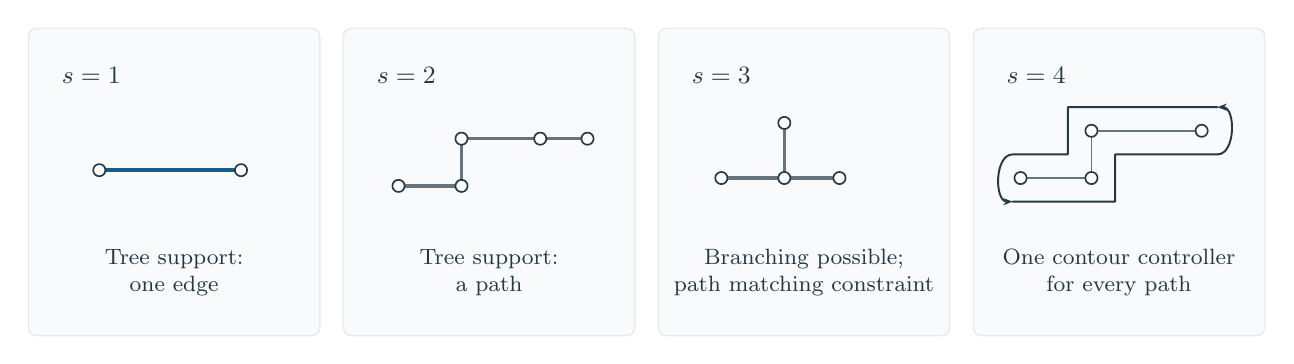
\begin{tikzpicture}[maze,x=1mm,y=1mm]
 \foreach \x in {0,40,80,120}{\draw[lightpanel] (\x,0) rectangle (\x+37,39);}
 \node[paneltitle] at (3,33) {$s=1$};
 \draw[supportA] (9,21)--(27,21); \node[cell] at (9,21) {}; \node[cell] at (27,21) {};
 \node[font=\footnotesize,align=center] at (18.5,8) {Tree support:\\one edge};
 \node[paneltitle] at (43,33) {$s=2$};
 \draw[edge,line width=1.2pt] (47,19)--(55,19)--(55,25)--(65,25)--(71,25);
 \foreach \x/\y in {47/19,55/19,55/25,65/25,71/25}{\node[cell] at (\x,\y) {};}
 \node[font=\footnotesize,align=center] at (58.5,8) {Tree support:\\a path};
 \node[paneltitle] at (83,33) {$s=3$};
 \draw[edge,line width=1.2pt] (88,20)--(96,20)--(103,20); \draw[edge,line width=1.2pt] (96,20)--(96,27);
 \foreach \x/\y in {88/20,96/20,103/20,96/27}{\node[cell] at (\x,\y) {};}
 \node[font=\footnotesize,align=center] at (98.5,8) {Branching possible;\\path matching constraint};
 \node[paneltitle] at (123,33) {$s=4$};
 \draw[edge] (126,20)--(135,20)--(135,26)--(149,26);
 \foreach \x/\y in {126/20,135/20,135/26,149/26}{\node[cell] at (\x,\y) {};}
 \draw[flow] (125,17)--(138,17)--(138,23)--(151,23) to[out=0,in=0] (151,29);
 \draw[flow] (151,29)--(132,29)--(132,23)--(125,23) to[out=180,in=180] (125,17);
 \node[font=\footnotesize,align=center] at (138.5,8) {One contour controller\\for every path};
\end{tikzpicture}
\caption{Memory constrains recurrent geometry: the first three panels summarize support capacity, while the last records the universal path controller of Section~\ref{sec:paths}. On three-state paths, matching is necessary; the compatibility theorem in Section~\ref{sec:realization} supplies the additional realization condition.}
\label{fig:memory-geometry}
\end{figure}


\subsection{Capacity of a tree support}

The number of internal states limits how much branching a recurrent tree support can carry.

\begin{theorem}[Support capacity]\label{thm:support-capacity}
Let $A$ be a compulsory-moving controller with $|Q_A|\le s$, and let $\Gamma$ be a primitive recurrent tagged cycle whose spatial support $T$ is a tree.  For each used edge $e$, let $k_e$ be the number of traversals of $e$ in either one of its two directions during one period, and let $r_v$ be the number of tags of $\Gamma$ lying over $v$.  Then
\[
 \boxed{r_v=\sum_{e\ni v}k_e\le s},
 \qquad
 \boxed{|\Gamma|=2\sum_{e\in E(T)}k_e},
 \qquad k_e\ge1.
\]
Consequently
\[
 \Delta(T)\le s,
\]
and for a square-grid support
\[
 \Delta(T)\le\min(s,4).
\]
\end{theorem}
\begin{proof}
Fix a used edge $e$.  Deleting $e$ separates $T$ into components $U$ and $W$.  During one closed period let $N_{UW}$ and $N_{WU}$ be the numbers of crossings of $e$ from $U$ to $W$ and from $W$ to $U$.  The indicator of the current vertex lying in $U$ returns to its initial value after one period, so its net change is zero.  Hence
\[
 N_{UW}=N_{WU}=:k_e.
\]
The edge belongs to the used support, so $k_e\ge1$.

Now fix $v\in V(T)$.  Every occurrence of $v$ in the cyclic spatial word has exactly one departure, because motion is compulsory.  Conversely every departure from $v$ corresponds to exactly one such occurrence.  Along each incident edge $e$, exactly $k_e$ traversals depart from $v$.  Therefore
\[
 r_v=\sum_{e\ni v}k_e.
\]
Since the tagged cycle is primitive, two occurrences over the same spatial vertex cannot carry the same state: otherwise that tag would repeat before the end of the period.  Thus $r_v\le |Q_A|\le s$.

Finally,
\[
 |\Gamma|=\sum_v r_v
 =\sum_v\sum_{e\ni v}k_e
 =2\sum_e k_e.
\]
Since every incident multiplicity is positive,
\[
 \deg_T(v)\le\sum_{e\ni v}k_e=r_v\le s.
\]
The grid contributes the independent degree bound four.
\end{proof}

Least period is essential for the capacity inequality: writing a cycle twice doubles $r_v$ without adding states. Theorem~\ref{thm:support-capacity} applies to the unique least tagged period of each recurrent trajectory.

\begin{corollary}[Low-state tree supports]\label{cor:low-state-tree-supports}
For a recurrent cycle with tree support in the compulsory-motion model:
\begin{enumerate}[label=(\roman*),leftmargin=2em]
 \item with one state, the support is a single edge;
 \item with two states, the support is a path;
 \item with three states, degree-three branching is no longer excluded by state capacity.
\end{enumerate}
\end{corollary}
\begin{proof}
A recurrent support contains at least one edge.  The first two claims follow from the bounds $\Delta(T)\le1$ and $\Delta(T)\le2$ for a connected tree.  For the third, the bound permits degree three, and the next sharpness construction realizes it.
\end{proof}

The degree bound is sharp on induced grid trees for every state budget up to the ambient degree.  Let $d=\min(s,4)$ and take a grid star with centre $c$ and leaves in distinct directions $d_0,\ldots,d_{d-1}$.  With states $0,\ldots,d-1$, define on the used rows
\[
 \delta(i,\{d_0,\ldots,d_{d-1}\})=(d_i,0),
 \qquad
 \delta(0,\{-d_i\})=(-d_i,i+1\!\!\pmod d).
\]
Completing the remaining rows arbitrarily gives the primitive cycle
\[
 c_0,\ell_{0,0},c_1,\ell_{1,0},\ldots,c_{d-1},\ell_{d-1,0},
\]
whose support has centre degree $d$.  Thus the local transition from path-like recurrence at $s=2$ to possible branching at $s=3$ is genuine.

\subsection{The sharp path period at every state budget}\label{sec:sharp-period}

Here $n$ counts vertices of the used support, not of a larger ambient maze.
The following bound is attained by a common mask table, so it is stronger than
optimizing the capacity inequalities in a vertex-dependent transition model.

\begin{theorem}[Sharp maximum path period]\label{thm:sharp-period}
For $s\ge2$ and $n\ge3$, the maximum least tagged period over all controllers with
at most $s$ states and all fully used $n$-vertex induced grid paths is
\[
 L_{\max}(s,n)=
 \begin{cases}
 sn-2,&n\text{ even},\\
 s(n-1),&n\text{ odd}.
 \end{cases}
\]
For a standalone two-vertex path, $L_{\max}(s,2)=2s$.
The displayed formula for $n\ge3$ is also an upper bound for any used path support
in a larger maze, regardless of the external masks. Attainment is asserted over
geometries and controllers, not on every fixed path.
\end{theorem}
\begin{proof}
Let $k_0,\ldots,k_{n-2}$ be the positive edge multiplicities.
When $n=2r+1$, partition the edges into $r$ consecutive pairs. Each pair has total
multiplicity at most $s$ by Theorem~\ref{thm:support-capacity}, whence
$L\le2rs=s(n-1)$. When $n=2r+2\ge4$, pair the first $2r$ edges in the same way.
The remaining edge has multiplicity at most $s-1$, since its neighbour has positive
multiplicity. Thus $L\le2(rs+s-1)=sn-2$.

For attainment put $p=s-1$ and take the monotone path with direction word
$\E\N\E\N\cdots$, beginning with $\E$. Every east edge has multiplicity $p$;
every north edge has multiplicity one. On its forward passage replace an east step
by $(\E\W)^{p-1}\E$; its backward passage is one west step. Use states
$0,1,\ldots,p$ and the following common internal-mask rows:
\[
\begin{array}{c|ccc}
 &0&1\le i<p&p\\\hline
 \E\Sdir &(\Sdir,p)&(\E,i)&(\E,0)\\
 \N\W &(\N,1)&(\W,i+1)&(\W,0)
\end{array}
\]
At the left endpoint, of mask $\E$, set $\delta(0,\E)=(\E,0)$ if $p=1$.
If $p\ge2$, use
\[
 \delta(0,\E)=(\E,1),\qquad
 \delta(i,\E)=(\E,i)\ (2\le i<p),\qquad
 \delta(p,\E)=(\E,0).
\]
For even $n$ the right endpoint has mask $\W$; use
$\delta(0,\W)=(\W,0)$ and
$\delta(i,\W)=(\W,i+1)$ for $1\le i<p$.
For odd $n$ it has mask $\Sdir$; use $\delta(1,\Sdir)=(\Sdir,p)$.
All other rows are completed by legal moves.

For an internal east edge $u\to v$, the forward tags are
\[
 (u_i,v_i)_{i=1}^{p-1},\quad u_p,v_0.
\]
The last tag moves north in state $1$. On the backward contour the next
$\E\Sdir$ vertex in state $0$ enters $v_p$, then $u_0$, and continues south.
Thus each internal vertex uses all $s$ states exactly once. At the left endpoint
replace the first $u_1$ by the starting tag $u_0$; the specified endpoint rows close
the same sequence. The left endpoint uses $p$ tags. The right uses $p$ tags for even
$n$ and one for odd $n$. All tags in the resulting closed word are distinct, giving
exactly the claimed least periods. This one table for each $s$ works at every length
of this alternating family.

On a standalone edge use $\delta(i,\E)=(\E,i)$ and
$\delta(i,\W)=(\W,i+1\bmod s)$ for $0\le i<s$. The resulting cycle has $2s$
distinct tags, attaining the capacity bound there as well.
\end{proof}

For one state no recurrent tree support can have $n\ge3$ vertices. For two states
all path multiplicities at $n\ge3$ are one, but not every prescribed contour is
realizable by a shared table. At three states the possible doubled edges form a
matching. Section~\ref{sec:realization} supplies the missing compatibility theorem;
the period bound by itself is not a realization criterion.



\subsection{Phase contact on a path}

The second structural ingredient is independent of automata.

\begin{theorem}[Phase contact]\label{thm:phase-contact}
Let $p:\mathbb Z\to\mathbb Z$ be periodic with period $L\ge1$ and satisfy
\[
 |p(t+1)-p(t)|\le1\qquad(t\in\mathbb Z).
\]
For any phase offsets $\alpha,\beta\in\mathbb Z$, there exists $t\in\{0,\ldots,L-1\}$ such that
\[
 \boxed{|p(t+\alpha)-p(t+\beta)|\le1.}
\]
\end{theorem}
\begin{proof}
Set $d(t)=p(t+\alpha)-p(t+\beta)$.  Then $|d(t+1)-d(t)|\le2$.  Suppose $|d(t)|\ge2$ for every $t$.  Since $d$ is integer-valued, its sign cannot change between consecutive times: a change from at least $2$ to at most $-2$, or conversely, would require a jump of magnitude at least four.  Periodicity therefore forces one strict sign throughout the whole cyclic period.  On the other hand, cyclic reindexing gives
\[
 \sum_{t=0}^{L-1}d(t)
 =\sum_{t=0}^{L-1}p(t+\alpha)-\sum_{t=0}^{L-1}p(t+\beta)=0,
\]
a contradiction.
\end{proof}

The theorem permits zero increments, so it remains true for lazy walks with WAIT.  It uses no state bound, no grid embedding, no simple tagged-cycle hypothesis, and no assumption that the ambient graph is a tree.

\begin{corollary}[Same-cycle contact on path support]\label{cor:same-cycle-path-contact}
Suppose two trajectories of the same controller eventually occupy phase shifts of one recurrent tagged cycle whose spatial support is a path.  Then at some integer time the two agents occupy the same or adjacent path vertices.
\end{corollary}
\begin{proof}
Choose an integer coordinate along the support path.  The projection of one period of the recurrent cycle is a periodic integer walk with step size at most one.  Once both trajectories lie on that cycle, they are two phase shifts of this word.  Theorem~\ref{thm:phase-contact} applies.
\end{proof}

Path support cannot be replaced by a branching-tree hypothesis. An explicit
three-state triod with a unique recurrent cycle and two eternally separated state-zero
trajectories is given in Appendix~\ref{app:branching-example}.

\section{Memoryless controllers at arbitrary radius}\label{sec:memoryless-radius}

The one-state case admits an exact controller-by-controller law for every success radius.  Its radius-one specialization recovers the exact one-state threshold.

\begin{theorem}[Memoryless radius law]\label{thm:memoryless-radius}
Let $A$ be any one-state controller and let $\rho\ge0$.  For each
\[
 \mathcal C\in\{\mathcal P,\mathcal J,\mathcal T_{\rm grid},\mathcal G\},
\]
one has
\[
 \boxed{
 \tau_{\mathcal C,\rho}(A)=F_{\mathcal C,\rho}(1)=
 \begin{cases}
 2,&0\le\rho<1,\\[1mm]
 \lfloor\rho\rfloor+3,&\rho\ge1.
 \end{cases}}
\]
In particular, within each of these four classes every memoryless controller has the same least trap size.
\end{theorem}
\begin{proof}
Write $k=\lfloor\rho\rfloor$.  By \eqref{eq:integer-radius}, radius $\rho$ and radius $k$ define exactly the same success event.

First suppose $0\le\rho<1$, so success means coincidence.  On a two-cell edge, agents started at opposite endpoints are forced to exchange endpoints forever and never coincide.  A singleton has only a time-zero success.  Every listed class contains the two-cell path, so the exact value is two.

Now let $k\ge1$.  We first prove a lower bound that does not use memorylessness.  If a connected maze $V$ with starts $x,y$ were a trap with $|V|\le k+2$, failure at time zero and connectedness would give
\[
 k+1\le d_1(x,y)\le d_V(x,y)\le |V|-1\le k+1.
\]
All inequalities are therefore equalities.  A shortest $x$--$y$ path has $|V|-1$ edges and visits every vertex.  Any extra edge joining nonconsecutive vertices of that path would shorten $d_V(x,y)$, so the whole maze graph is that induced path, with $x,y$ as its endpoints.  Compulsory motion forces both first moves inward.  If the path is
\[
 x=v_0,v_1,\ldots,v_k,v_{k+1}=y,
\]
then after one round the agents are at $v_1$ and $v_k$, and
\[
 d_1(v_1,v_k)\le d_V(v_1,v_k)=k-1\le k\le\rho.
\]
Thus every controller succeeds on every connected maze of at most $k+2$ cells.

It remains to give a matching trap for an arbitrary one-state rule.  Write $r(M)\in M$ for the chosen direction at mask $M$ and set
\[
 h=r(\{\E,\W\}),\qquad v=r(\{\N,\Sdir\}).
\]
The unit vectors $h$ and $v$ are perpendicular.  On the corner mask $\{h,v\}$ let
\[
 a=r(\{h,v\}),\qquad \{a,b\}=\{h,v\}.
\]
Then
\[
 r(\{a,b\})=a,\qquad r(\{b,-b\})=b.
\]
Consider
\[
 V_k=\{0,a,b,2b,\ldots,(k+1)b\},
\]
whose path order is $a,0,b,2b,\ldots,(k+1)b$.  This is an induced path with $k+3$ cells.  Start the two agents at $a$ and $kb$.  The endpoint move from $a$ is forced, the corner at $0$ chooses $a$, an interior $b$-arm cell chooses $b$, and the outer endpoint is forced back.  Hence
\[
 (a,kb)\longleftrightarrow(0,(k+1)b).
\]
Both configurations have Manhattan separation $k+1>\rho$, so they form a trap.  The same witness belongs to all four listed maze classes.
\end{proof}

% Abstract a/b preferred directions. Horizontal ellipsis denotes omitted cells.
\begin{figure}[tbp]
\centering
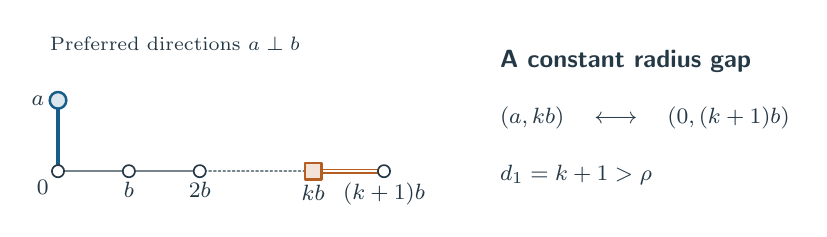
\begin{tikzpicture}[maze,x=9mm,y=9mm]
 \coordinate (z) at (0,0); \coordinate (a) at (0,1);
 \coordinate (b1) at (1,0); \coordinate (b2) at (2,0);
 \coordinate (bk) at (3.6,0); \coordinate (bkp) at (4.6,0);
 \draw[supportA] (a)--(z); \draw[quiet] (z)--(b1)--(b2);
 \draw[quiet,densely dotted] (b2)--(bk); \draw[supportB] (bk)--(bkp);
 \node[cell,label=below left:{$0$}] at (z) {};
 \node[startA,label=left:{$a$}] at (a) {};
 \node[cell,label=below:{$b$}] at (b1) {}; \node[cell,label=below:{$2b$}] at (b2) {};
 \node[startB,label=below:{$kb$}] at (bk) {}; \node[cell,label=below:{$(k+1)b$}] at (bkp) {};
 \node[font=\scriptsize,anchor=west] at (-.25,1.8) {Preferred directions $a\perp b$};
 \node[paneltitle] at (6.1,1.55) {A constant radius gap};
 \node[note] at (6.1,.75) {$(a,kb)\quad\longleftrightarrow\quad(0,(k+1)b)$};
 \node[note] at (6.1,-.05) {$d_1=k+1>\rho$};
\end{tikzpicture}
\caption{Memoryless trap for $k=\lfloor\rho\rfloor\ge1$, with starts at $a$ and $kb$. The axes are preferred directions, not absolute compass labels; the long arm is schematic, with intermediate labels coalescing for $k=1,2$.}
\label{fig:memoryless-l-trap}
\end{figure}


The class restriction in Theorem~\ref{thm:memoryless-radius} concerns only the matching upper witness: the small-maze lower bound holds for every class of connected induced grid mazes, while equality follows for any class containing the controller-adapted path $V_k$.

\begin{corollary}[The original one-state threshold]\label{cor:one-state-radius-one}\label{thm:A}
For the original radius-one model,
\[
 F_{\mathcal P,1}(1)=F_{\mathcal J,1}(1)
 =F_{\mathcal T_{\rm grid},1}(1)=F(1)=4.
\]
\end{corollary}

Thus the value four is the first nontrivial instance of the general law $\lfloor\rho\rfloor+3$, rather than a separate low-state phenomenon requiring its own proof.

\section{Exact two-state traps in grid mazes}\label{sec:two-state}

The general capacity and contact lemmas isolate the recurrent part of the argument,
but the exact threshold also requires control of transients and of the distinguished
initial state. We prove both bounds without computational assistance.

\begin{theorem}[Exact two-state trap threshold]\label{thm:B}\label{thm:C}
For synchronous radius-one rendezvous in the stated model,
\[
 F(2)=F_{\mathcal J,1}(2)=F_{\mathcal T_{\rm grid},1}(2)=7.
\]
Every controller with at most two states has a trap of at most seven cells that is
an induced path or a tree with exactly one degree-three vertex. The controller
$\Astar$ below succeeds on every connected induced grid maze through six cells and
has a seven-cell induced-path trap.
\end{theorem}

The upper argument first constrains the table by path
witnesses and then uses a junction; it does not assert a paths-only upper bound of
seven. The lower argument treats subcubic trees structurally before exhausting the
remaining geometries through six cells.

\subsection{A seven-cell tree obstruction}\label{u:section}

We prove a slightly sharper upper bound than required: every controller
with at most two states has a trap of size at most seven that is either
an induced path or an induced tree with one vertex of degree three.
Throughout this section, an action is written
$\delta(q,M)=(d,r)$, with direction first. We call a controller a
\emph{path survivor} if it succeeds from every pair of state-zero starts
on every induced grid path with at most seven cells.

Two elementary observations will certify the traps. If two executions
stay in regions whose cross-distances are at least two, they cannot
succeed. If instead their regions are merely disjoint, the same conclusion
holds when their starts have equal checkerboard color: compulsory
synchronous motion preserves equality of their colors, whereas adjacent
cells have different colors. In every application below the regions
contain the initial positions, or an explicit entry prefix is given.

All compass normalizations act on the controller as well as on the
maze. For $g\in D_4$, define
\[
 (g\delta)(q,gM)=(gd,r)\quad\text{when }\delta(q,M)=(d,r).
\]
Induction on time conjugates the complete tagged executions under
$(x,q)\mapsto(gx,q)$. Manhattan distance and initial state zero are
preserved. In particular, a trap for the transported controller gives
a trap for the original controller by applying $g^{-1}$.

\subsubsection{Straight-axis rigidity}

\begin{lemma}[Axis reduction]\label{u:axis}
For a path survivor, one simultaneous compass symmetry makes the
straight rows
\[
\begin{array}{ll}
\delta(0,\mathrm{NS})=(\Sdir,f_v(0)),&
\delta(1,\mathrm{NS})=(\N,f_v(1)),\\
\delta(0,\mathrm{EW})=(\W,f_h(0)),&
\delta(1,\mathrm{EW})=(\E,f_h(1)).
\end{array}
\]
Each map $f=f_v,f_h$ is a constant map $C_0,C_1$ or the identity $I$.
Write $L_q$ for the next-state bit at the negative endpoint of an axis
and $R_q$ for that at its positive endpoint. The necessary restrictions are
\[
\begin{array}{c|l}
f&\text{endpoint restrictions}\\ \hline
C_0&L_0=1,\ R_0=0,\\
I&L_0=1,\ (R_0,R_1)\ne(1,1),\\
C_1&L_1=1,\ (R_0,R_1)\ne(1,1).
\end{array}\tag{\ref{u:axis}a}
\]
All unlisted endpoint bits remain arbitrary.
\end{lemma}

\begin{proof}
For perpendicular unit directions $d,e$, the seven cells
\[
 U(d,e)=\{0,e,2e,d,2d,2e+d,2e+2d\}
\]
form an induced path with two parallel two-edge arms pointing in direction
$d$. If both straight rows on an axis choose $d$, starts at $d$ and
$2e+d$ stay on translated terminal edges, regardless of all next-state
bits. Their distance is always two. Thus the straight directions are
opposite, and independent coordinate reflections give the displayed
normalization without exchanging the states.

Index a straight path by increasing coordinates. If $f=(1,0)$, the
six-cell path $0,\ldots,5$ with starts $2,4$ gives the two tagged cycles
$(2_0,1_1)$ and $(4_0,3_1)$; the agents remain two cells apart.
If $f=C_0$ and $R_0=1$, the five-cell path $0,\ldots,4$ with starts
$0,4$ confines the right agent to $(4_0,3_1)$ and the left to $0,1,2$.
Indeed the left word is $(0_0,1_0)^\infty$ when $L_0=0$, and
$(0_0,1_1,2_0,1_0)^\infty$ when $L_0=1$.
The regions are disjoint and the starts have equal color.
If $f=C_1$ and $L_1=0$, use the same line with starts $1,3$.
The left cycle is $(1_0,0_1)$; the right prefix
$3_0\to2_1\to3_1$ enters the closed region $2,3,4$.
At its positive endpoint, either return bit keeps it in that region.
Again equal colors exclude adjacency.

Two terminal-edge tests finish the restrictions. If $L_{f(0)}=0$,
an inner state-zero start has cycle
$I_0\to E_{f(0)}\to I_0$ at a negative terminal edge. Two copies
in $U(d,e)$, with $d$ negative and inner starts, give a trap.
If $R_0=R_{f(1)}=1$, an endpoint start at a positive terminal edge has
word $E_0\to I_1\to E_{f(1)}\to I_1\to\cdots$.
Clone these words in the positive-pointing $U(d,e)$, with endpoint
starts. Both constructions keep the agents two units apart.
The four possible two-bit maps, together with these exclusions, give
exactly the necessary restrictions displayed above.
\end{proof}

For singleton masks write
$\delta(q,\N)=(\N,n_q)$, and similarly $e_q,s_q,w_q$.
Thus $(L,R)=(n,s)$ vertically and $(e,w)$ horizontally.
For perpendicular directions $u,v$, put
\[
 L(u,v;a,b)=\{C,u_1,\ldots,u_a,v_1,\ldots,v_b\},
 \qquad C=(0,0),\quad d_j=jd.
\]
This is an induced path with $a+b+1$ cells.

\begin{lemma}[Reset pocket]\label{u:pocket}
Suppose a straight state map resets to $\kappa$, and let $d$ be the
direction selected by state $\kappa$. On a terminal arm
$C,d_1,d_2,d_3$, a state-zero start at $d_2$ never reaches $C$.
\end{lemma}

\begin{proof}
The tagged set
$\{(d_1)_\kappa,(d_2)_0,(d_2)_1,(d_3)_\kappa\}$ is closed.
At $d_2$, either action reaches $d_1$ or $d_3$ in state $\kappa$.
From $(d_1)_\kappa$ the next move goes outward to $(d_2)_\kappa$;
the endpoint $(d_3)_\kappa$ returns to $d_2$ in either state.
The set contains the initial tagged position.
\end{proof}

% Exact geometry: C=(0,0), S_j=(0,-j); other neighbours of C omitted.
\begin{figure}[tbp]
\centering
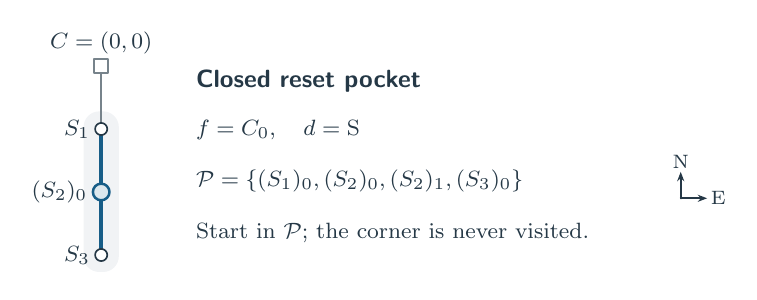
\begin{tikzpicture}[maze,x=8mm,y=8mm]
 \fill[rvGray!60,rounded corners=2mm] (-.28,-3.27) rectangle (.28,-.72);
 \draw[quiet] (0,0)--(0,-1);
 \draw[supportA] (0,-1)--(0,-2)--(0,-3);
 \node[gate,label=above:{$C=(0,0)$}] at (0,0) {};
 \node[cell,label=left:{$S_1$}] at (0,-1) {};
 \node[startA,label=left:{$(S_2)_0$}] at (0,-2) {};
 \node[cell,label=left:{$S_3$}] at (0,-3) {};
 \node[paneltitle] at (1.35,-.25) {Closed reset pocket};
 \node[note] at (1.35,-1.02) {$f=C_0,\quad d=\Sdir$};
 \node[note] at (1.35,-1.82) {$\mathcal P=\{(S_1)_0,(S_2)_0,(S_2)_1,(S_3)_0\}$};
 \node[note] at (1.35,-2.65) {Start in $\mathcal P$; the corner is never visited.};
 \mazeCompass{9.2}{-2.1}
\end{tikzpicture}
\caption{The closed tagged pocket for reset state $0$ and direction $\Sdir$; unshown neighbours of $C$ do not affect it. Other reset directions transport both the geometry and the controller directions together.}
\label{f:reset-pocket}
\end{figure}


\begin{lemma}[Straight-axis rigidity]\label{u:rigidity}
For a path survivor in the frame of Lemma~\ref{u:axis}, both
straight state maps are the identity. Consequently
\[
 n_0=e_0=1,
 \qquad (s_0,s_1),(w_0,w_1)\ne(1,1).
\]
\end{lemma}

\begin{proof}
If both axes reset, choose their outward reset directions $d_v,d_h$.
On $L(d_v,d_h;3,3)$ start at $(d_v)_2,(d_h)_2$.
Lemma~\ref{u:pocket} confines the agents to different three-cell
arms, whose cross-distances are at least two. This treats all four
choices of the two reset bits.

If exactly one axis resets, interchange the axes simultaneously to
make it vertical. The two remaining possibilities are
$C_0/I$ and $C_1/I$. Lemmas~\ref{u:mixed0} and~\ref{u:mixed1}
give explicit path obstructions for each in
Appendix~\ref{u:appendix-mixed}. Their proofs use reset pockets,
closed arms, and short transition words; all endpoint bits allowed by
Lemma~\ref{u:axis} are retained. Thus neither mixed possibility can
survive. The endpoint conclusions now follow from Lemma~\ref{u:axis}.
\end{proof}

\subsubsection{Corner compatibility and a nine-entry pattern}

\begin{lemma}[Corner arrival]\label{u:arrival}
Use the normalized straight directions of Lemma~\ref{u:axis}.
Let $C,I,E$ be a terminal arm of two edges, with $I$ a straight cell
and direction $d$ from $C$ into the arm. Every arrival at $C$ from
this arm has state $a_d=f(q_{-d})$, where state $q_{-d}$ selects the
straight direction toward $C$. If the corner action in state $a_d$
points back into the arm, a state-zero start at $I$ remains in
$C,I,E$. For identity straight maps,
\[
a_\N=a_\E=0,\qquad a_\Sdir=a_\W=1.
\]
\end{lemma}

\begin{proof}
The last move $I\to C$ gives the arrival formula. Endpoints return
to $I$, straight moves stay in the arm or reach $C$ in that state,
and the specified corner row sends such an arrival back to $I$.
This proves closure from the stated initial position, with no
restriction on endpoint or corner output bits.
\end{proof}

Call the condition in this lemma a \emph{locked arm}. Two corners
two units apart, joined by their middle cell, can carry perpendicular
two-edge arms on either side of the connector. If both arms are locked,
starts at their inner cells stay in parallel rows or columns two
units apart. Each construction is an induced seven-cell path.

\begin{lemma}[Corner compatibility]\label{u:corners}
After one further diagonal reflection, a path survivor satisfies
\[
\begin{array}{ll}
\delta(0,\mathrm{NE})=(\E,1),&
\delta(0,\mathrm{ES})=(\Sdir,0),\\
\delta(1,\mathrm{ES})=(\E,1),&
\delta(1,\mathrm{SW})=(\Sdir,0).
\end{array}\tag{\ref{u:corners}a}
\]
\end{lemma}

\begin{proof}
The diagonal reflection exchanges the axes, preserves the four
identity straight rows, and lets us choose the direction of
$\delta(0,\mathrm{NE})$ to be $\E$. Its east arm is locked.
The following three paired-arm obstructions force the other directions.
First put an NE corner at $(0,0)$ with east arm and an SW corner at
$(0,2)$ with west arm, joined through $(0,1)$. If SW in state 1
chose west, both arms would be locked. Hence SW in state 1 chooses
south. Next replace the upper corner by ES with an east arm; if ES
in state 0 chose east, both east arms would be locked. Thus ES in
state 0 chooses south. Finally use $U(\Sdir,\E)$: its two corners
have masks ES and SW. The SW south arm is locked, so ES in state 1
cannot also choose south. It must choose east. Starts in all three
constructions are the inner cells of the two arms.

These direction conclusions leave four output bits. The four
six-cell obstructions in Lemma~\ref{u:bit-laws} force them to be,
respectively, $1,0,1,0$. Each argument uses disjoint regions and
equal-color starts, and none assumes any of the other three bit
conclusions.
\end{proof}

% Exact six-cell grid geometry; highlighted regions are closed, not fixed cycles.
\begin{figure}[tbp]
\centering
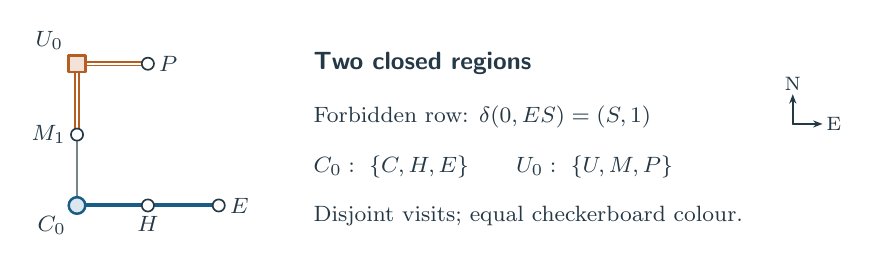
\begin{tikzpicture}[maze,x=9mm,y=9mm]
 \coordinate (P) at (1,2); \coordinate (U) at (0,2);
 \coordinate (M) at (0,1); \coordinate (C) at (0,0);
 \coordinate (H) at (1,0); \coordinate (Eend) at (2,0);
 \draw[quiet] (M)--(C);
 \draw[supportB] (P)--(U)--(M);
 \draw[supportA] (C)--(H)--(Eend);
 \node[cell,label=right:{$P$}] at (P) {};
 \node[startB,label=above left:{$U_0$}] at (U) {};
 \node[cell,label=left:{$M_1$}] at (M) {};
 \node[startA,label=below left:{$C_0$}] at (C) {};
 \node[cell,label=below:{$H$}] at (H) {};
 \node[cell,label=right:{$E$}] at (Eend) {};
 \node[paneltitle] at (3.2,2.0) {Two closed regions};
 \node[note] at (3.2,1.25) {Forbidden row: $\delta(0,ES)=(S,1)$};
 \node[note] at (3.2,.55) {$C_0:\ \{C,H,E\}\qquad U_0:\ \{U,M,P\}$};
 \node[note] at (3.2,-.15) {Disjoint visits; equal checkerboard colour.};
 \mazeCompass{10.1}{1.15}
\end{tikzpicture}
\caption{Corner obstruction under the stated forbidden row and preceding rigidity hypotheses. The $U$-started execution reaches $M$ only in state $1$; disjointness excludes coincidence and parity excludes adjacency.}
\label{f:corner-path}
\end{figure}


\begin{lemma}[Nine-entry pattern]\label{u:nine}
Every path survivor admits a simultaneous compass frame in which
the following entries hold:
\[
\begin{array}{c|c|c@{\qquad}c|c|c}
M&q&\delta(q,M)&M&q&\delta(q,M)\\ \hline
\N&0&(\N,1)&\mathrm{NE}&1&(\N,1)\\
\E&0&(\E,1)&\mathrm{ES}&0&(\Sdir,0)\\
\W&1&(\W,1)&\mathrm{ES}&1&(\E,1)\\
\mathrm{EW}&1&(\E,1)&\mathrm{SW}&1&(\Sdir,0)\\
\mathrm{NE}&0&(\E,1)&&&
\end{array}\tag{\ref{u:nine}a}
\]
No junction entry is prescribed.
\end{lemma}

\begin{proof}
Only $w_1=1$ and $\delta(1,\mathrm{NE})=(\N,1)$ remain to be
proved. Use the path, in endpoint order,
\[
 (1,0),(0,0),(0,1),(0,2),(1,2),(2,2),(2,1),
\]
with state-zero starts $A=(0,0)$ and $Q=(2,1)$.
Put $P=(1,0)$, $M=(0,1)$, and $D=(2,2)$.
The right agent has cycle $Q_0\to D_1\to Q_0$.
The left starts $A_0\to P_1$. If $w_1=0$, it returns to $A_0$
and repeats. If $w_1=1$, it reaches $A_1$. Should the NE state-one
row choose east, $A,P$ is closed; should it be $(\N,0)$, its only
extra excursion is $A_1\to M_0\to A_0$. In every bad case the
left stays in $A,P,M$, all at distance at least two from $Q,D$.
Thus the two remaining entries are forced, and the other seven
come from Lemmas~\ref{u:rigidity} and~\ref{u:corners}.
\end{proof}

% Exact seven-cell path. Left highlight is a conditional closed region.
\begin{figure}[tbp]
\centering
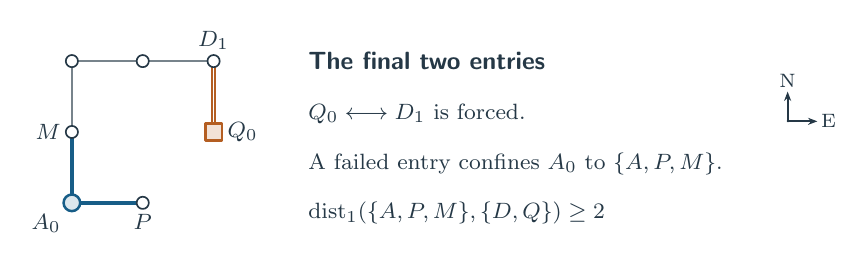
\begin{tikzpicture}[maze,x=9mm,y=9mm]
 \coordinate (P) at (1,0); \coordinate (A) at (0,0);
 \coordinate (M) at (0,1); \coordinate (T) at (0,2);
 \coordinate (H) at (1,2); \coordinate (D) at (2,2);
 \coordinate (Q) at (2,1);
 \draw[quiet] (M)--(T)--(H)--(D);
 \draw[supportA] (P)--(A)--(M); \draw[supportB] (Q)--(D);
 \node[cell,label=below:{$P$}] at (P) {};
 \node[startA,label=below left:{$A_0$}] at (A) {};
 \node[cell,label=left:{$M$}] at (M) {};
 \node[cell] at (T) {}; \node[cell] at (H) {};
 \node[cell,label=above:{$D_1$}] at (D) {};
 \node[startB,label=right:{$Q_0$}] at (Q) {};
 \node[paneltitle] at (3.2,2.0) {The final two entries};
 \node[note] at (3.2,1.25) {$Q_0\longleftrightarrow D_1$ is forced.};
 \node[note] at (3.2,.55) {A failed entry confines $A_0$ to $\{A,P,M\}$.};
 \node[note] at (3.2,-.15) {$\operatorname{dist}_1(\{A,P,M\},\{D,Q\})\ge2$};
 \mazeCompass{10.1}{1.15}
\end{tikzpicture}
\caption{The final seven-cell path, anchored at $A=(0,0)$. If either remaining W9 entry fails, the left execution stays separated from the forced right-hand tagged two-cycle, including the transient.}
\label{f:final-path}
\end{figure}


\subsubsection{Completion at a junction}

The last step uses only the nine entries of Lemma~\ref{u:nine}; all
other rows remain arbitrary.

\begin{lemma}[Junction completion]\label{u:junction}
Every legal completion of the nine-entry pattern has a trap on one
of the two seven-cell induced trees $G_1,G_2$ below.
\end{lemma}

\begin{proof}
Write $\delta(1,\E)=(\E,\epsilon)$ and
$u=\delta(0,\mathrm{NSW})$, $v=\delta(1,\mathrm{NSW})$.
The common cells of the two trees are
\[
A=(0,1),\quad B=(1,0),\quad J=(1,1),\quad
U=(1,2),\quad V=(2,2).
\]
For $G_1$ add $D=(2,0),F=(3,0)$ and start at $A,B$.
For $G_2$ add $Q=(3,1),R=(3,2)$ and start at $B,Q$.
All starts have state zero. The edge sets are
\[
\begin{array}{c|l}
G_1&JA,JB,JU,UV,BD,DF,\\
G_2&JA,JB,JU,UV,VR,RQ.
\end{array}
\]
Direct coordinate comparison gives no other unit-distance pair.
Each tree has one degree-three vertex $J$, with mask NSW.
Choose $G_2$ precisely when
\[
 v=(\Sdir,0)\quad\text{or}\quad
 \bigl[u=(\Sdir,0)\text{ and }
 v\in\{(\N,0),(\W,1)\}\bigr].\tag{\ref{u:junction}a}
\]
Choose $G_1$ otherwise.

On $G_1$, the B-started agent follows
$B_0\to D_1\to F_1\to D_1\to\cdots$.
The A-started agent begins $A_0\to J_1$. Its relevant nonjunction
transitions are
\[
\begin{gathered}
A_0\to J_1,\quad A_1\to J_\epsilon,\quad B_1\to J_1,\\
U_0\to J_0,\quad U_1\to V_1,\quad V_1\to U_1.
\end{gathered}
\]
If neither $u$ nor $v$ is $(\Sdir,0)$, these transitions and the
allowed junction departures close the tagged set
\[
\{A_0,A_1,J_0,J_1,B_1,U_0,U_1,V_1\}.
\]
The remaining $G_1$ cases have $u=(\Sdir,0)$ and
$v\in\{(\N,1),(\Sdir,1),(\W,0)\}$.
They send the A-started agent, respectively, to the edge $UV$, to
the state-one cycle on $JB$, or to $J_1\leftrightarrow A_0$.
It never queries $J_0$, so the row $u$ is harmless.
Thus from time one the two agents lie on disjoint regions, one on
$DF$ and the other outside it. At time zero they are distinct and
have equal checkerboard color, which excludes adjacency at every
time. Hence $G_1$ is a trap in every case where it was selected.

On $G_2$ the Q-started cycle is always $Q_0\leftrightarrow R_1$.
The selection condition gives exactly the following B-started words:
\[
\begin{array}{l|l}
v=(\Sdir,0)&(B_0,J_1)^\infty\\
u=(\Sdir,0),\ v=(\N,0)&(B_0,J_1,U_0,J_0)^\infty\\
u=(\Sdir,0),\ v=(\W,1),\ \epsilon=0
 &(B_0,J_1,A_1,J_0)^\infty\\
u=(\Sdir,0),\ v=(\W,1),\ \epsilon=1
 &B_0,(J_1,A_1)^\infty.
\end{array}
\]
Every indicated move is fixed by the nine entries or the displayed
choice of $u,v,\epsilon$. At each integer time the distance from
the other agent is exactly three, as follows directly from the
coordinates. This includes all transients and finishes the proof.
\end{proof}

% Both embeddings retain the exact coordinates from the original junction proof.
\begin{figure}[tbp]
\centering
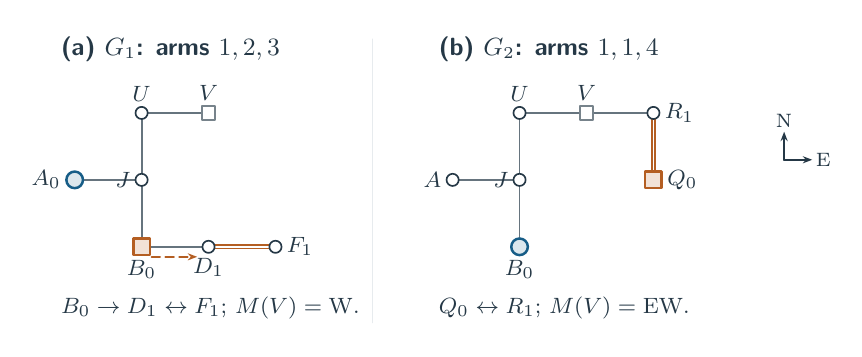
\begin{tikzpicture}[maze,x=8.5mm,y=8.5mm]
 \begin{scope}
  \coordinate (A) at (0,1); \coordinate (B) at (1,0); \coordinate (J) at (1,1);
  \coordinate (U) at (1,2); \coordinate (V) at (2,2); \coordinate (D) at (2,0); \coordinate (F) at (3,0);
  \draw[edge] (A)--(J)--(B)--(D)--(F); \draw[edge] (J)--(U)--(V);
  \draw[supportB] (D)--(F); \draw[transientB] (1.15,-.15)--(1.83,-.15);
  \node[startA,label=left:{$A_0$}] at (A) {};
  \node[startB,label=below:{$B_0$}] at (B) {};
  \node[cell,label=left:{$J$}] at (J) {}; \node[cell,label=above:{$U$}] at (U) {};
  \node[gate,label=above:{$V$}] at (V) {}; \node[cell,label=below:{$D_1$}] at (D) {};
  \node[cell,label=right:{$F_1$}] at (F) {};
  \node[paneltitle] at (-.35,2.95) {(a) $G_1$: arms $1,2,3$};
  \node[note] at (-.35,-.92) {$B_0\to D_1\leftrightarrow F_1$; $M(V)=\W$.};
 \end{scope}
 \draw[rvGray,line width=.65pt] (4.45,-1.13)--(4.45,3.1);
 \begin{scope}[xshift=48mm]
  \coordinate (A) at (0,1); \coordinate (B) at (1,0); \coordinate (J) at (1,1);
  \coordinate (U) at (1,2); \coordinate (V) at (2,2); \coordinate (Q) at (3,1); \coordinate (R) at (3,2);
  \draw[edge] (A)--(J)--(B); \draw[edge] (J)--(U)--(V)--(R);
  \draw[supportB] (Q)--(R);
  \node[cell,label=left:{$A$}] at (A) {}; \node[startA,label=below:{$B_0$}] at (B) {};
  \node[cell,label=left:{$J$}] at (J) {}; \node[cell,label=above:{$U$}] at (U) {};
  \node[gate,label=above:{$V$}] at (V) {}; \node[startB,label=right:{$Q_0$}] at (Q) {};
  \node[cell,label=right:{$R_1$}] at (R) {};
  \node[paneltitle] at (-.35,2.95) {(b) $G_2$: arms $1,1,4$};
  \node[note] at (-.35,-.92) {$Q_0\leftrightarrow R_1$; $M(V)=\E\W$.};
 \end{scope}
 \mazeCompass{10.6}{1.3}
\end{tikzpicture}
\caption{Junction completions with $J=(1,1)$ and $M(J)=\N\Sdir\W$. The highlighted right-hand shuttle is fixed in each selected case; the other execution is governed by the exact alternatives in the proof.}
\label{f:junctions}
\end{figure}


\begin{proposition}[Upper bound in a narrow tree class]\label{u:upper}
Every controller with at most two states has a trap with at most
seven cells that is either an induced path or an induced tree with
exactly one vertex of degree three and no larger degree. In particular,
$F(2)\le7$ and $F_{\mathrm{grid\ trees}}(2)\le7$.
\end{proposition}

\begin{proof}
A two-state controller either already has a path trap of size at
most seven, or is a path survivor. In the second case apply
Lemma~\ref{u:nine}, then Lemma~\ref{u:junction}, and transport the
resulting tree and starts back by the inverse compass symmetry.
A one-state controller can be extended by a legal unused second
state without changing any execution from its distinguished initial
state. The two-state argument therefore covers it as well.
\end{proof}

\subsection{An extremal controller and its seven-cell trap}\label{sec:extremal}

Table~\ref{tab:astar} specifies all thirty entries of $\Astar$, with direction first and updated state second.

\begin{table}[!htbp]
\centering
\begin{tabular}{@{}llll@{}}
\toprule
Mask type & Mask & State $0$ & State $1$\\
\midrule
End & $\N$ & $(\N,0)$ & $(\N,1)$\\
 & $\E$ & $(\E,1)$ & $(\E,1)$\\
 & $\Sdir$ & $(\Sdir,1)$ & $(\Sdir,1)$\\
 & $\W$ & $(\W,1)$ & $(\W,0)$\\
Straight & $\N\Sdir$ & $(\Sdir,1)$ & $(\Sdir,1)$\\
 & $\E\W$ & $(\W,0)$ & $(\E,1)$\\
Corner & $\N\E$ & $(\N,0)$ & $(\E,1)$\\
 & $\E\Sdir$ & $(\Sdir,1)$ & $(\E,1)$\\
 & $\Sdir\W$ & $(\W,0)$ & $(\Sdir,1)$\\
 & $\N\W$ & $(\N,1)$ & $(\W,0)$\\
Junction & $\N\E\Sdir$ & $(\Sdir,1)$ & $(\E,1)$\\
 & $\N\E\W$ & $(\W,0)$ & $(\E,1)$\\
 & $\N\Sdir\W$ & $(\Sdir,0)$ & $(\Sdir,0)$\\
 & $\E\Sdir\W$ & $(\Sdir,1)$ & $(\Sdir,1)$\\
Full & $\N\E\Sdir\W$ & $(\E,0)$ & $(\Sdir,1)$\\
\bottomrule
\end{tabular}
\caption{The extremal controller $\Astar$. Every direction belongs to its mask. The distinguished initial state is $0$.}
\label{tab:astar}
\end{table}

On a vertical straight segment both states move south and reset to $1$. On a horizontal straight segment state $0$ moves west and state $1$ moves east, each preserving its state. The masks $\N\E\Sdir$ and $\N\E\W$ behave like $\E\Sdir$ and $\E\W$, respectively, so their extra northern arms are never selected. The remaining three-way masks also avoid north. These local asymmetries will determine the possible recurrent supports.

\begin{lemma}[Seven-cell sharpness witness]\label{a:trap}
The controller $\Astar$ has a trap on the induced path
\[
 V_U=\{(0,0),(0,1),(0,2),(1,2),(2,2),(2,1),(2,0)\},
\]
with state-$0$ starts at $(0,0)$ and $(2,0)$.
\end{lemma}
\begin{proof}
The bottom cells have mask $\N$, and their northern neighbours have mask $\N\Sdir$. The entire execution through the first repeated product state is
\[
\begin{array}{c|c|c|c}
t&\text{first agent}&\text{second agent}&\text{distance}\\\hline
0&(0,0)_0&(2,0)_0&2\\
1&(0,1)_0&(2,1)_0&2\\
2&(0,0)_1&(2,0)_1&2\\
3&(0,1)_1&(2,1)_1&2\\
4&(0,0)_1&(2,0)_1&2
\end{array}
\]
Time $4$ repeats time $2$. Determinism gives separation two forever, including the transient. The product preperiod and period are both exactly two.
\end{proof}

% Exact U witness for Astar. Phase labels are copied from Lemma a:trap.
\begin{figure}[tbp]
\centering
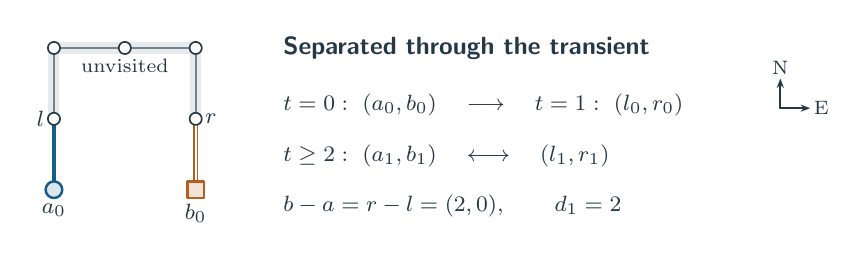
\begin{tikzpicture}[maze,x=9mm,y=9mm]
 \coordinate (a) at (0,0); \coordinate (l) at (0,1);
 \coordinate (c) at (0,2); \coordinate (m) at (1,2);
 \coordinate (d) at (2,2); \coordinate (r) at (2,1);
 \coordinate (b) at (2,0);
 \draw[rvGray,line width=4pt] (l)--(c)--(m)--(d)--(r);
 \draw[quiet] (l)--(c)--(m)--(d)--(r);
 \draw[supportA] (a)--(l); \draw[supportB] (b)--(r);
 \foreach \p in {l,c,m,d,r} {\node[cell] at (\p) {};}
 \node[font=\footnotesize,left] at (l) {$l$};
 \node[font=\footnotesize,right] at (r) {$r$};
 \node[startA,label=below:{$a_0$}] at (a) {};
 \node[startB,label=below:{$b_0$}] at (b) {};
 \node[font=\scriptsize,fill=white,inner sep=1pt] at (1,1.75) {unvisited};
 \node[paneltitle] at (3.1,2.0) {Separated through the transient};
 \node[note] at (3.1,1.20) {$t=0:\ (a_0,b_0)\quad\longrightarrow\quad t=1:\ (l_0,r_0)$};
 \node[note] at (3.1,.48) {$t\ge2:\ (a_1,b_1)\quad\longleftrightarrow\quad(l_1,r_1)$};
 \node[note] at (3.1,-.23) {$b-a=r-l=(2,0),\qquad d_1=2$};
 \mazeCompass{10.25}{1.15}
\end{tikzpicture}
\caption{The seven-cell U-trap for $A^\star$, with $a=(0,0)$ and $b=(2,0)$. The upper connector is never visited; from time $2$ both executions shuttle in state $1$ on the highlighted edges.}
\label{f:astar-u}
\end{figure}


For the lower bound, we prove that $\Astar$ succeeds through six cells. Tagged recurrence matters: visits to one cell can carry different states, and separated eventual supports may still force transient contact.

\subsection{Recurrent supports on trees}\label{sec:tree-lower}

We first separate elementary contact principles from the special features of
\(\Astar\). A \emph{tagged cycle} means a simple directed cycle of
\(\Phi_V\), and its \emph{support} consists of the spatial vertices and edges
used by that tagged cycle. In particular, the support does not include an
ambient edge merely because both its endpoints occur. A tagged cycle is
\emph{reachable} if some initial tag \((x,0)\), \(x\in V\), eventually enters it.
We call a support \emph{long} if it has at least two edges.

\begin{lemma}[Two-state path support]\label{t:path-support}
For any compulsory-moving controller with at most two states, a primitive tagged cycle whose support is a tree has nonempty path support.  If that path has $a\ge2$ edges, the tagged cycle traverses each edge once in each direction and has period $2a$.  On a one-edge support the tagged period is two or four.
\end{lemma}
\begin{proof}
The path-support conclusion is Corollary~\ref{cor:low-state-tree-supports}.  If the path has at least two edges, an internal vertex $v$ has two incident support edges.  Theorem~\ref{thm:support-capacity} gives
\[
 2\le \sum_{e\ni v}k_e=r_v\le2,
\]
so both incident multiplicities equal one.  Propagation along the connected path gives $k_e=1$ on every edge, and Theorem~\ref{thm:support-capacity} then gives period $2a$.  On a single edge, $r_v=k_e\le2$, so $k_e\in\{1,2\}$ and the period is $2$ or $4$.
\end{proof}

\begin{lemma}[Contact on one tagged cycle]\label{t:same-cycle}
If two trajectories eventually enter the same tagged cycle and its support is a path, they achieve distance-one contact.  Their initial tags and entry times may be arbitrary, and the ambient maze need not be a tree.
\end{lemma}
\begin{proof}
This is Corollary~\ref{cor:same-cycle-path-contact}.
\end{proof}

\begin{lemma}[Contact through an edge support]\label{t:edge-contact}
Suppose one eventual tagged cycle is supported on an edge \(uv\), and the
other eventual tagged cycle visits \(u\) or \(v\). The trajectories achieve
distance-one contact, independently of their entry times and phases.
\end{lemma}
\begin{proof}
After both transients have ended, the first agent is always at \(u\) or
\(v\). At any subsequent visit of the second agent to the shared endpoint,
their distance is at most one. Such visits recur.
\end{proof}

\begin{lemma}[Order inversion]\label{t:order-inversion}
Two synchronous nearest-neighbour walks on a path cannot reverse their
strict spatial order without first achieving distance-one contact.
In particular, contact occurs if their eventual disjoint support intervals
occur in the opposite order from their initial positions.
\end{lemma}
\begin{proof}
In path coordinates the difference of their positions changes by at most
two at each step. As long as its absolute value is at least two, its sign
cannot reverse. This proves the assertion, including the whole transient.
\end{proof}

The support hypothesis in Lemma~\ref{t:same-cycle} and the edge hypothesis
in Lemma~\ref{t:edge-contact} will be established before either lemma is
applied. Neither contact nor equality of spatial positions requires equality
of the internal states.

\subsubsection{A north-boundary invariant}

For a support in a tree, call an edge from a support vertex to a vertex
outside the support a \emph{boundary edge}, directed away from the support.
All directions in the following statements refer to the fixed compass of
Table~\ref{tab:astar}.

\begin{lemma}[Exclusion of a full vertex]\label{t:no-full}
On an induced grid tree, a long tagged cycle of \(\Astar\) contains no
vertex with mask \(NESW\).
\end{lemma}
\begin{proof}
Suppose first that a full vertex \(p\) occurs in state \(1\).
Its next tag is \(s_1\), where \(s\) is its southern neighbour.
If \(s\) is internal to the support, one of its two support exits is north,
and its state-\(1\) exit must continue away from \(p\). The only masks
with two distinct exits including north are \(NE\) and \(NW\).
Accordingly \(s\) has an eastern or western neighbour. That neighbour,
\(s\), \(p\), and the corresponding eastern or western neighbour of \(p\)
form a unit square, contradicting inducedness and the tree hypothesis.
If \(s\) is a support endpoint, returning north from state \(1\) requires
mask \(N\) and returns to \(p_1\). This closes a two-tag cycle, contradicting
long support.

A full vertex occurring only in state \(0\) must be a support endpoint,
by Lemma~\ref{t:path-support}. Its eastern neighbour is internal and is
entered in state \(0\). To continue away from \(p\) in that state and
return west in the other state, this neighbour must have mask \(NW\).
Its northern neighbour and the northern neighbour of \(p\) again complete
a unit square. This excludes the remaining case.
\end{proof}

\begin{lemma}[North boundary]\label{t:north-boundary}
For \(\Astar\) on any finite induced grid tree, every boundary edge of a
long tagged cycle points north.
\end{lemma}
\begin{proof}
An internal support vertex uses both states and selects its two support
edges. The masks with distinct selected directions are
\(NE,ES,NW,EW,SW,NES,NEW,NESW\).
Lemma~\ref{t:no-full} excludes \(NESW\). The mask \(NW\) is also impossible
internally: to pass from its western support neighbour towards its
northern support neighbour, the vertex must be entered in state \(0\).
Every eastward move from a non-full vertex arrives in state \(1\), whereas
the predecessor cannot be full.

The remaining internal possibilities are displayed below. Here \(d/r\)
denotes direction \(d\) and new state \(r\), in the convention
\(\delta(q,M)=(d,r)\). The last column lists only neighbours outside the
two selected support edges.
\begin{center}
\small
\begin{tabular}{@{}llll@{}}
\toprule
Internal mask & From \(0\) & From \(1\) & Possible boundary port\\
\midrule
\(EW,NEW\) & \(\W/0\) & \(\E/1\) & \(N\), for \(NEW\)\\
\(NE\) & \(\N/0\) & \(\E/1\) & none\\
\(SW\) & \(\W/0\) & \(\Sdir/1\) & none\\
\(ES,NES\) & \(\Sdir/1\) & \(\E/1\) & \(N\), for \(NES\)\\
\bottomrule
\end{tabular}
\end{center}
It remains to check support endpoints; no global assumption about the
shape of the path is needed. Let \(c\) be an endpoint and \(v\) its adjacent
internal support vertex.

If \(v\) is east of \(c\), its westward return enters \(c\) in state \(0\).
To avoid immediately repeating that return, the eastward move from \(c\)
must arrive at \(v\) in state \(1\). Only an \(E\) leaf, used in state \(0\),
does so.
If \(v\) is west of \(c\), its eastward return enters \(c\) in state \(1\);
the westward return from \(c\) must arrive at \(v\) in state \(0\).
Exactly \(W\) and \(NW\) in state \(1\) have this behaviour.

If \(v\) is north of \(c\), its southward move arrives at \(c_1\).
The only state-\(1\) northward move is from an \(N\) leaf and arrives in
state \(1\). The internal neighbour cannot be \(SW\), since this would
repeat the same two tags immediately; it is \(ES\) or \(NES\).
Finally, if \(v\) is south of \(c\), then \(v\) has mask \(NE\), whose
northward move enters \(c_0\). The southward return must arrive at \(v\)
in state \(1\).
The candidate masks at \(c\) are \(S,NS,ES,NES,ESW\). Each of the last
three requires an eastern neighbour; together with \(c,v\), and the
eastern support neighbour of \(v\), it forms a unit square. Only
\(S\) and \(NS\) remain.

These four directional equations give the complete endpoint table.
\begin{center}
\small
\begin{tabular}{@{}llll@{}}
\toprule
Endpoint mask & Tag & Direction to support & Boundary port\\
\midrule
\(E\) & \(0\) & \(E\) & none\\
\(N\) & \(1\) & \(N\), towards \(ES/NES\) & none\\
\(S,NS\) & \(0\) & \(S\), towards \(NE\) & \(N\), for \(NS\)\\
\(W,NW\) & \(1\) & \(W\) & \(N\), for \(NW\)\\
\bottomrule
\end{tabular}
\end{center}
Every boundary port in the two tables points north.
\end{proof}

Both preceding lemmas are independent of maze size and of maximum degree.
Inducedness is used when a required fourth side turns a local configuration
into a spatial square.

\subsubsection{Short supports and the six-cell budget}

\begin{lemma}[Edge profiles]\label{t:edge-profiles}
Every edge-supported tagged cycle of \(\Astar\), on any maze, has period
two and belongs to one of the five rows of Table~\ref{t:edge-table}.
On a connected induced tree with more than two cells and maximum degree
at most three, these reduce to the five port profiles in
Table~\ref{t:profile-table}. None has a south-pointing boundary edge.
\end{lemma}
\begin{proof}
A four-tag horizontal cycle would require both states at the western
endpoint to move east. Only an \(E\) leaf does this, and both moves arrive
in state \(1\), which precludes four distinct tags. A four-tag vertical
cycle requires an \(N\) leaf at the lower endpoint. At its upper endpoint
both states must move south, and every such mask resets the state to a
constant. This again precludes four distinct tags.

For period two, solve the two endpoint equations in the semantic table.
For example, a lower state-\(0\) tag that moves north as \(0\) has mask
\(N\) or \(NE\); the upper tag returns south as \(0\) precisely with mask
\(NSW\). This gives the first row. A lower \(0\) that arrives north as
\(1\) requires \(NW\), and its upper \(1\) must return south as \(0\),
again with \(NSW\). A lower \(1\) moving north requires \(N\), and its
upper \(1\) must move south as \(1\), giving the third row. Horizontally,
an eastward arrival as \(0\) requires the full western vertex in state
\(0\), followed by a state-\(0\) westward return; an eastward arrival as
\(1\) followed by return to western state \(0\) requires the western
\(E\) leaf and an eastern \(W\) or \(NW\) tag in state \(1\).
A western tag in state \(1\) would require a westward arrival as \(1\),
which is available only from an eastern \(W\) leaf in state \(0\);
no state-\(1\) eastward move can return to that eastern tag in state \(0\).
These are all possible state pairs and directions.

\begin{table}[!htbp]
\centering
\small
\begin{tabular}{@{}lll@{}}
\toprule
Orientation; endpoint tags & Western/lower mask & Eastern/upper mask\\
\midrule
Vertical; \(0,0\) & \(N,NE\) & \(NSW\)\\
Vertical; \(0,1\) & \(NW\) & \(NSW\)\\
Vertical; \(1,1\) & \(N\) & \(S,NS,SW,ESW,NESW\)\\
Horizontal; \(0,0\) & \(NESW\) & \(EW,NEW,SW\)\\
Horizontal; \(0,1\) & \(E\) & \(W,NW\)\\
\bottomrule
\end{tabular}
\caption{All local edge-supported tagged cycles of \(\Astar\). The two
tags are ordered west--east or south--north.}\label{t:edge-table}
\end{table}

The second row forces western neighbours at both endpoints and therefore
a unit square; it is excluded on an induced tree. The fourth row and
the full-mask option of the third are excluded by the degree bound.
A horizontal \(E\)--\(W\) pair or a vertical \(N\)--\(S\) pair forms an
entire two-cell connected component, excluded by the size assumption.
The remaining possibilities are exactly Table~\ref{t:profile-table}.
\end{proof}

\begin{table}[!htbp]
\centering
\small
\begin{tabularx}{\linewidth}{@{}l l l X c@{}}
\toprule
Profile & Tail/head masks & Tagged cycle & Boundary ports & Cells required\\
\midrule
\(H\) & \(E;NW\) & \(u_0,h_1\) & \(N\) at \(h\) & \(1\)\\
\(D_N\) & \(N;NS\) & \(u_1,h_1\) & \(N\) at \(h\) & \(1\)\\
\(D_W\) & \(N;SW\) & \(u_1,h_1\) & \(W\) at \(h\) & \(1\)\\
\(D_{EW}\) & \(N;ESW\) & \(u_1,h_1\) & \(E,W\) at \(h\) & \(2\)\\
\(Z\) & \(N\) or \(NE;NSW\) & \(u_0,h_0\) &
\(N,W\) at \(h\), and \(E\) at \(u\) if \(u\) has mask \(NE\) & \(2\) or \(3\)\\
\bottomrule
\end{tabularx}
\caption{The five edge profiles on subcubic induced trees with more than
two cells. The tail \(u\) lies west of the head \(h\) in \(H\), and south
of it otherwise. The last column counts required cells outside the
two-cell support, before a connecting path is chosen.}\label{t:profile-table}
\end{table}

\begin{lemma}[Disjointness of recurrent supports]\label{t:disjoint}
Distinct tagged cycles of \(\Astar\) on a subcubic induced grid tree have
disjoint spatial supports.
\end{lemma}
\begin{proof}
An internal support vertex uses both tags and cannot occur on a second
tagged cycle. A shared spatial vertex must therefore be an endpoint of
both supports, in opposite states. The endpoint table in the proof of
Lemma~\ref{t:north-boundary} allows no mask in both endpoint states, so
two long supports cannot intersect.

Comparing that table with Table~\ref{t:profile-table} leaves two possible
mask coincidences for a long and an edge support. An \(NS\) endpoint in
state \(0\) could coincide with a \(D_N\) head in state \(1\), but its
southern neighbour would have to be both an internal \(NE\) vertex and
an \(N\) leaf. An \(N\) endpoint in state \(1\) could coincide with the
lower \(Z\) endpoint in state \(0\), but its northern neighbour would
have to be both \(ES/NES\) and \(NSW\). Neither is possible.
For two edge supports the only opposite-state coincidence is an \(N\)
tail in states \(0\) and \(1\); its upper neighbour would require mask
\(NSW\) for the former and \(NS,SW,\) or \(ESW\) for the latter.
Thus it is impossible as well. The two-cell maze has only its single
edge cycle, so it creates no omitted exception.
\end{proof}

\begin{lemma}[Uniqueness of a long support through six]\label{t:long-unique}
If \(|V|\le6\), \(V\) is a subcubic induced grid tree, and \(\Astar\)
has a long tagged cycle on \(V\), it has no other tagged cycle.
\end{lemma}
\begin{proof}
By Lemma~\ref{t:disjoint}, another support would be disjoint. A long
support has only north boundary edges, whereas any other support has
no south boundary edge, by Lemmas~\ref{t:north-boundary}
and~\ref{t:edge-profiles}. Direct adjacency between the supports is
therefore impossible. Their unique connecting path has an intermediate
vertex.

Two long supports require at least \(3+3+1=7\) vertices. A long support
of at least four vertices paired with an edge support also requires
at least seven. The only remaining budget is a three-vertex long
support, a two-vertex edge support, and one connecting vertex.
An edge profile \(D_{EW}\) or \(Z\) requires another branch off this
minimal union, giving a seventh vertex. For \(H\) or \(D_N\), both
boundary ports are north, so the two-step connector would be \(NS\)
and return to its starting point. For \(D_W\), it must be \(NE\).
The southern support leaf of the \(D_W\) head is then adjacent to the
starting support vertex. It either overlaps the long support or closes
a unit square. Every case is excluded.
\end{proof}

\begin{lemma}[The four short-support configurations]\label{t:four-patterns}
If a subcubic induced grid tree of at most six cells contains two
edge-supported tagged cycles of \(\Astar\), then, up to translation,
it is exactly one of the four six-cell sets in
Table~\ref{t:pattern-coordinates}. Each has exactly two tagged cycles.
\end{lemma}
\begin{proof}
The supports are disjoint by Lemma~\ref{t:disjoint}. Let their unique
connector have \(k\) edges, excluding the two support edges themselves.
The union already has \(k+3\) vertices. A required port off this union
costs a further distinct vertex: identifying that neighbour with the
union would create a spatial cycle. A connector attached to a
\(D_{EW}\) head has one such extra cost. At a \(Z\) head the cost is
one; when it attaches at the eastern port of the lower \(Z\) vertex,
the cost is two. The other profiles have no extra cost after their
unique boundary port has been selected.

The resulting fifteen unordered comparisons are recorded in
Table~\ref{t:pair-table}. Connector words are read from the first named
profile to the second. Exchanging their names only relabels the
connector endpoints and does not transform compass directions.

\begin{table}[!htbp]
\centering
\small
\begin{tabularx}{\linewidth}{@{}l l X@{}}
\toprule
Profile pair & Budget & Outcome\\
\midrule
\(H,H\) & \(k\le3\) & North--north obstruction\\
\(H,D_N\) & \(k\le3\) & North--north obstruction\\
\(D_N,D_N\) & \(k\le3\) & North--north obstruction\\
\(D_W,D_W\) & \(k\le3\) & West--west obstruction\\
\(H,D_W\) & \(k\le3\) & Only \(NEE\); gives \(P_H\)\\
\(D_N,D_W\) & \(k\le3\) & Only \(NEE\); gives \(P_N\)\\
\(H,D_{EW}\) & \(k\le2\) & Square or overlapping supports\\
\(D_N,D_{EW}\) & \(k\le2\) & Square\\
\(D_W,D_{EW}\) & \(k\le2\) & Only \(WW\); gives \(P_E\)\\
\(D_{EW},D_{EW}\) & \(k\le1\) & Adjacent southern leaves close a square\\
\(H,Z\) & \(k\le2\) at head; \(\le1\) below &
Square at head; incompatible lower-port directions\\
\(D_N,Z\) & \(k\le2\) at head; \(\le1\) below &
Square at head; incompatible lower-port directions\\
\(D_W,Z\) & \(k\le2\) at head; \(\le1\) below &
Square at head; direct \(W\) into the lower vertex gives \(P_Z\)\\
\(D_{EW},Z\) & \(k\le1\) at head &
Square; lower attachment exceeds the budget\\
\(Z,Z\) & \(k\le1\) between heads &
No compatible direct ports; other attachments exceed the budget\\
\bottomrule
\end{tabularx}
\caption{All fifteen pairings of the five edge profiles. The proof gives
the direction and square obstruction behind every rejected row. No
compass orientations are identified.}\label{t:pair-table}
\end{table}

Here are the complete route arguments. Two north ports require a
connector beginning \(N\) and ending \(S\). At length at most three,
the only simple possibilities are \(NES,NWS\); their endpoint heads
are horizontally adjacent, so the induced edge closes a square.
Shorter possibilities revisit a vertex. For two west ports the
corresponding words are \(WNE,WSE\), and the vertically adjacent
heads again close a square. A north port joined to a west port
requires final step \(E\). The length-two word \(NE\) closes a
square through the second head's southern leaf. At length three,
\(NNE\) closes the same square one level higher, and \(NEE\) is the
only other simple word. This proves the first six rows.

A \(D_{EW}\) attachment requires a horizontal final step. From a north
port, the budget allows only \(NE\) or \(NW\); the southern support
leaf of the second head is adjacent to the first head, closing a
square or overlapping a support. From a west port, a one-step
connection makes the southern leaves adjacent and closes a square;
among two-step words, \(WE\) repeats the starting vertex and \(WW\)
survives. Two \(D_{EW}\) heads have only the already excluded one-step
geometry. This proves rows seven through ten.

A \(Z\) head accepts outside neighbours north and west, so a connector
entering it ends in \(S\) or \(E\). From a north port with \(k\le2\),
the only simple word is \(NE\), which closes a square through the
lower \(Z\) support vertex. From a west port, \(WE\) repeats the start,
and \(WS\) closes a square through the first head's southern leaf.
Direct westward entry would approach the forbidden eastern side of
the \(Z\) head. At the lower \(Z\) endpoint the outside port is east;
the two extra head neighbours force \(k\le1\), and the one-step
westward connection matches only a \(D_W\) head. A \(D_{EW}\)--\(Z\)
head connection has only one step available: its compatible horizontal
direction again leaves adjacent southern support vertices and hence
a square. Connecting instead to the lower \(Z\) vertex would need
at least seven cells. Finally, a direct \(Z\)--\(Z\) head connector
would have to begin in \(N\) or \(W\) and end in \(S\) or \(E\), which
is impossible in one step; any use of a lower port exceeds the
budget. This proves the remaining five rows.

\begin{table}[!htbp]
\centering
\small
\begin{tabular}{@{}ll@{}}
\toprule
Pattern & Cell set\\
\midrule
\(P_N\) & \(\{(0,-1),(0,0),(0,1),(1,1),(2,1),(2,0)\}\)\\
\(P_E\) & \(\{(-1,0),(0,-1),(0,0),(1,0),(2,0),(2,-1)\}\)\\
\(P_Z\) & \(\{(0,0),(0,1),(0,2),(-1,1),(1,0),(1,-1)\}\)\\
\(P_H\) & \(\{(-1,0),(0,0),(0,1),(1,1),(2,1),(2,0)\}\)\\
\bottomrule
\end{tabular}
\caption{The four possible subcubic six-cell trees with two tagged
cycles. Coordinates retain absolute orientation.}\label{t:pattern-coordinates}
\end{table}

The surviving words and required port cells give exactly the four
displayed sets. Their masks satisfy the stated edge profiles, so
both tagged cycles exist, and no additional branch fits. A third tagged cycle
would have disjoint support and use only the two vertices outside
the first two supports. In \(P_N,P_H\), those two vertices have
masks \(ES,EW\), which do not form any row of Table~\ref{t:edge-table}.
In \(P_E,P_Z\), they are not adjacent. Thus there is no third tagged
cycle, including one supported on connector vertices.
\end{proof}

\subsubsection{Initial-state gates and transient contact}

Two spatially separated tagged cycles do not by themselves constitute a
trap. We must determine which state-\(0\) roots reach them and whether
the approach trajectories have already contacted.

\begin{lemma}[Three closed state-\(0\) gates]\label{t:reset-gates}
In each of \(P_N,P_E,P_Z\), every state-\(0\) root reaches the same
tagged cycle.
\end{lemma}
\begin{proof}
In all three patterns the right cycle is the state-\(1\) vertical edge
at a \(D_W\) head \(r\) and its southern \(N\) leaf \(b\). However,
\(r_0\) moves west as \(0\), and \(b_0\) first enters \(r_0\).
These are escape routes from the right support.

For \(P_N\), put \(\ell=(0,0)\), \(a=(0,-1)\), \(p=(0,1)\),
\(m=(1,1)\), \(r=(2,1)\), and \(b=(2,0)\). The \(NS\) head
\(\ell\) sends both states south into the cycle
\((\ell_1,a_1)\). Every state-\(0\) root reaches it, as witnessed by
\[
 a_0\to\ell_0\to a_1,\qquad
 p_0\to\ell_1,\qquad
 m_0\to p_0,\qquad r_0\to m_0,\qquad b_0\to r_0.
\]
The potentially east-going tag \(p_1\) is never reached by a
state-\(0\) root.

For \(P_E\), put \(\ell=(0,0)\), \(a=(0,-1)\), \(w=(-1,0)\),
\(m=(1,0)\), \(r=(2,0)\), and \(b=(2,-1)\). The \(ESW\) head
\(\ell\) sends both states to \(a_1\), and the left cycle is
\((\ell_1,a_1)\). The remaining roots satisfy
\[
 w_0\to\ell_1,\qquad a_0\to\ell_0,\qquad
 m_0\to\ell_0,\qquad r_0\to m_0,\qquad b_0\to r_0.
\]
Thus every root again enters the left cycle.

For \(P_Z\), write \(z=(0,0)\), \(t=(0,1)\), \(n=(0,2)\),
\(w=(-1,1)\), \(r=(1,0)\), \(b=(1,-1)\).
The left cycle is \((z_0,t_0)\). The leaves \(n,w\) both enter
\(t_1\), and the \(NSW\) rule sends that tag to \(z_0\).
The other roots are on the cycle or satisfy
\[
 r_0\to z_0,\qquad b_0\to r_0.
\]
Consequently the east-going tag \(z_1\) is unreachable from the
distinguished initial state.
\end{proof}

\begin{lemma}[The exceptional path]\label{t:exceptional-path}
All pairs of state-\(0\) roots on \(P_H\) achieve distance-one contact.
\end{lemma}
\begin{proof}
Name its vertices
\[
 w=(-1,0),\quad h=(0,0),\quad p=(0,1),\quad
 m=(1,1),\quad r=(2,1),\quad b=(2,0).
\]
Their induced path order is \(w,h,p,m,r,b\).
The complete twelve-tag map is
\begin{center}
\small
\begin{tabular}{@{}llll@{}}
\toprule
Cell & Mask & From \(0\) & From \(1\)\\
\midrule
\(w\) & \(E\) & \(h_1\) & \(h_1\)\\
\(h\) & \(NW\) & \(p_1\) & \(w_0\)\\
\(p\) & \(ES\) & \(h_1\) & \(m_1\)\\
\(m\) & \(EW\) & \(p_0\) & \(r_1\)\\
\(r\) & \(SW\) & \(m_0\) & \(b_1\)\\
\(b\) & \(N\) & \(r_0\) & \(r_1\)\\
\bottomrule
\end{tabular}
\end{center}
Its two tagged cycles are \(L=(w_0,h_1)\) and \(R=(r_1,b_1)\).
The only state-\(0\) root reaching \(R\) is \(h_0\), along
\(h_0\to p_1\to m_1\to r_1\). Every other root reaches \(L\):
\(w_0\) lies on it and \(p_0,m_0,r_0,b_0\) move successively
left towards it.

Pairs in the same basin contact by Lemma~\ref{t:same-cycle}.
For a cross-basin pair, one root is \(h\). Its only predecessor
in path order is \(w\), which is initially adjacent. Every other
root lies to the right of \(h\), yet its eventual support \(L\)
lies to the left of \(R\). These walks reverse their strict order
and therefore contact by Lemma~\ref{t:order-inversion}.
The argument includes all entry times and the complete transients.
\end{proof}

% The only marked start is h_0. L and R denote cycle supports, not two starts.
\begin{figure}[tbp]
\centering
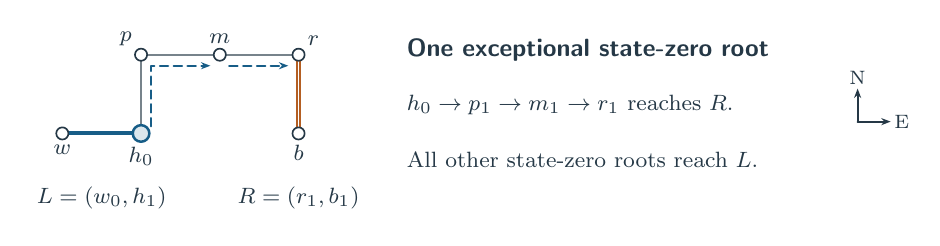
\begin{tikzpicture}[maze,x=10mm,y=10mm]
 \coordinate (w) at (-1,0); \coordinate (h) at (0,0);
 \coordinate (p) at (0,1); \coordinate (m) at (1,1);
 \coordinate (r) at (2,1); \coordinate (b) at (2,0);
 \draw[quiet] (h)--(p)--(m)--(r);
 \draw[supportA] (w)--(h); \draw[supportB] (r)--(b);
 \node[cell,label=below:{$w$}] at (w) {};
 \node[startA,label=below:{$h_0$}] at (h) {};
 \node[cell,label=above left:{$p$}] at (p) {};
 \node[cell,label=above:{$m$}] at (m) {};
 \node[cell,label=above right:{$r$}] at (r) {};
 \node[cell,label=below:{$b$}] at (b) {};
 \draw[transientA] (.13,.09)--(.13,.86)--(.88,.86);
 \draw[transientA] (1.12,.86)--(1.87,.86);
 \node[font=\footnotesize,anchor=north] at (-.5,-.55) {$L=(w_0,h_1)$};
 \node[font=\footnotesize,anchor=north] at (2,-.55) {$R=(r_1,b_1)$};
 \node[paneltitle] at (3.25,1.05) {One exceptional state-zero root};
 \node[note] at (3.25,.36) {$h_0\to p_1\to m_1\to r_1$ reaches $R$.};
 \node[note] at (3.25,-.33) {All other state-zero roots reach $L$.};
 \mazeCompass{9.1}{.15}
\end{tikzpicture}
\caption{The exceptional path $P_H$, in order $w,h,p,m,r,b$ with $h=(0,0)$. The dashed route is the unique state-zero entry to $R$; initially far pairs in different basins must reverse their spatial order before settling.}
\label{f:exceptional-path}
\end{figure}


\begin{samepage}
\begin{proposition}[Small subcubic trees]\label{t:small-trees}
Two copies of \(\Astar\), both started in state \(0\), achieve
distance-one contact on every induced grid tree of maximum degree
at most three with at most six cells.
\end{proposition}
\begin{proof}
The one- and two-cell cases succeed at time zero. On a larger
finite tree every trajectory eventually enters a tagged cycle,
whose support is a path by Lemma~\ref{t:path-support}.
If a long support exists, its tagged cycle is unique by
Lemma~\ref{t:long-unique}, so Lemma~\ref{t:same-cycle} applies.
If all supports are edges, there is either one tagged cycle,
handled by the same lemma, or the maze is one of the four
configurations of Lemma~\ref{t:four-patterns}.
Lemma~\ref{t:reset-gates} and then Lemma~\ref{t:same-cycle}
handle \(P_N,P_E,P_Z\); Lemma~\ref{t:exceptional-path}
handles \(P_H\).
\end{proof}
\end{samepage}

Trees containing a degree-four vertex are covered by the full-centre
analysis below. The distinction matters: at such a vertex, two
different tagged cycles may share a spatial endpoint in opposite
states, a configuration excluded by Lemma~\ref{t:disjoint} only under
its stated degree bound.

\subsection{The remaining small mazes}\label{sec:cyclic}

We now account for full vertices and spatial cycles. This part of the proof
works for arbitrary initial tags. Compass directions remain absolute
throughout: translations are used to name cells, but no rotation of the fixed
controller \(\Astar\) is assumed.

\begin{lemma}[Small-maze geometry]\label{c:geometry}
Every connected induced grid maze with \(3\le |V|\le6\) belongs to exactly one
of the following structural families, with \(\mathsf X\) given priority:
\(\mathsf X\), a full vertex, its four neighbours, and at most one further
cell; \(\mathsf T\), a tree of maximum degree at most three;
\(\mathsf Q\), a unit square with at most two attached tree cells, with no
full vertex and no second square; or \(\mathsf R\), either absolute
orientation of the \(2\times3\) rectangle.
\end{lemma}
\begin{proof}
A degree-four vertex already accounts for five cells, so connectivity gives
\(\mathsf X\). In its absence an acyclic maze belongs to \(\mathsf T\).
A shortest spatial cycle in the remaining maze has length four or six,
because the grid is bipartite. A simple six-edge grid cycle has two vertical
and four horizontal edges, or four vertical and two horizontal edges. In the
first case the two vertical edges join two adjacent rows, and each row
contributes the straight two-edge segment between their endpoints. The six
vertices form a \(3\times2\) rectangle. Inducedness supplies its middle
vertical edge, and hence a unit square. Interchanging the roles of the axes
proves the same geometric assertion in the other case.

Thus a unit square is present and at most two cells remain. If these cells
create another spatial cycle, they supply a three-edge detour between two
adjacent square vertices. A one-cell exterior detour is impossible: the
common grid neighbours of opposite square vertices are already in the
square. The three-edge detour supplies a second unit square sharing an
edge with the first, and their union is a \(2\times3\) rectangle. Otherwise
the remaining cells are trees attached at single square vertices, giving
\(\mathsf Q\). The four families are disjoint under the stated priority.
\end{proof}

% Four exact baseline representatives; all grid units are 7 mm.
\begin{figure}[tbp]
\centering
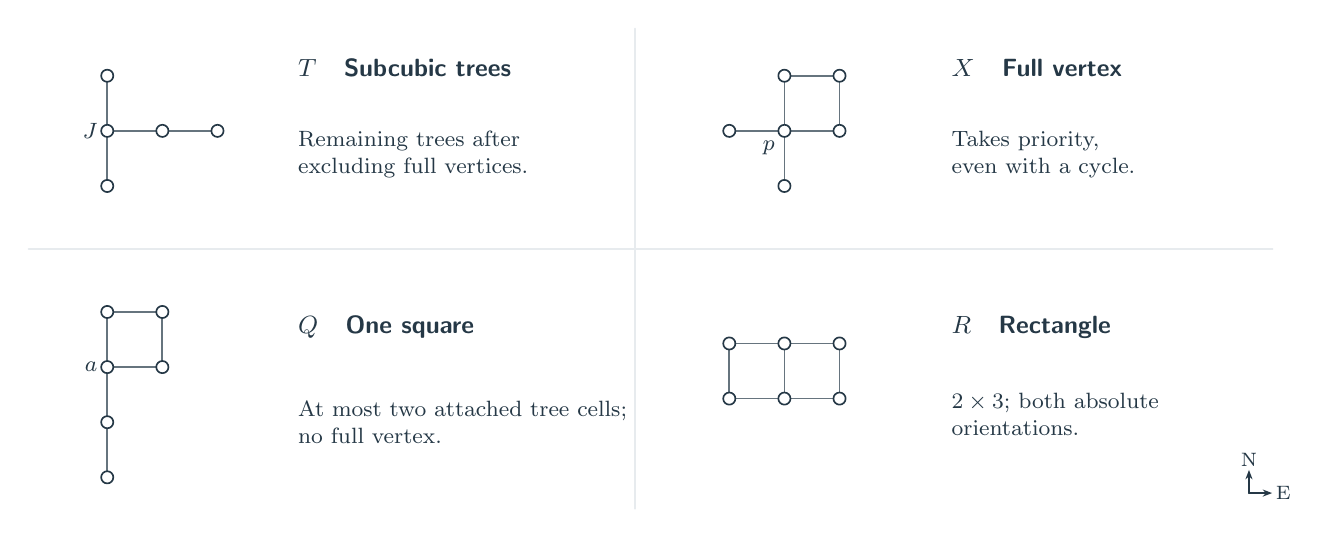
\begin{tikzpicture}[maze,x=1mm,y=1mm]
 \draw[rvGray,line width=.6pt] (77,-10)--(77,51);
 \draw[rvGray,line width=.6pt] (0,23)--(158,23);
 \begin{scope}[shift={(10,31)},x=7mm,y=7mm]
  \draw[edge] (0,0)--(0,1)--(0,2); \draw[edge] (0,1)--(1,1)--(2,1);
  \foreach \x/\y in {0/0,0/1,0/2,1/1,2/1}{\node[cell] at (\x,\y) {};}
  \node[font=\footnotesize,left] at (0,1) {$J$};
 \end{scope}
 \node[paneltitle] at (33,46) {$T$\quad Subcubic trees};
 \node[note] at (33,35) {Remaining trees after\\excluding full vertices.};
 \begin{scope}[shift={(96,38)},x=7mm,y=7mm]
  \draw[edge] (-1,0)--(0,0)--(1,0)--(1,1)--(0,1)--(0,0)--(0,-1);
  \foreach \x/\y in {0/0,0/1,1/0,0/-1,-1/0,1/1}{\node[cell] at (\x,\y) {};}
  \node[font=\footnotesize,below left] at (0,0) {$p$};
 \end{scope}
 \node[paneltitle] at (116,46) {$X$\quad Full vertex};
 \node[note] at (116,35) {Takes priority,\\even with a cycle.};
 \begin{scope}[shift={(10,8)},x=7mm,y=7mm]
  \draw[edge] (0,0)--(1,0)--(1,1)--(0,1)--(0,0)--(0,-1)--(0,-2);
  \foreach \x/\y in {0/0,1/0,1/1,0/1,0/-1,0/-2}{\node[cell] at (\x,\y) {};}
  \node[font=\footnotesize,left] at (0,0) {$a$};
 \end{scope}
 \node[paneltitle] at (33,13) {$Q$\quad One square};
 \node[note] at (33,1) {At most two attached tree cells;\\no full vertex.};
 \begin{scope}[shift={(89,4)},x=7mm,y=7mm]
  \draw[edge] (0,0)--(1,0)--(2,0)--(2,1)--(1,1)--(0,1)--(0,0);
  \draw[edge] (1,0)--(1,1);
  \foreach \x/\y in {0/0,1/0,2/0,0/1,1/1,2/1}{\node[cell] at (\x,\y) {};}
 \end{scope}
 \node[paneltitle] at (116,13) {$R$\quad Rectangle};
 \node[note] at (116,2) {$2\times3$; both absolute\\orientations.};
 \begin{scope}[shift={(155,-8)},x=7mm,y=7mm]\mazeCompass{0}{0}\end{scope}
\end{tikzpicture}
\caption{The structural partition for $3\le |V|\le6$, at a common grid scale. These are geometric families, not compass symmetry classes; no start pair is selected.}
\label{f:maze-families}
\end{figure}


\begin{lemma}[Full-centre routing]\label{c:full-centre}
On every maze in \(\mathsf X\), two copies of \(\Astar\) rendezvous from
arbitrary initial tags.
\end{lemma}
\begin{proof}
Translate the full vertex to \(p=(0,0)\), and write
\(n=(0,1),e=(1,0),s=(0,-1),w=(-1,0)\). If a sixth cell \(x\) is present,
it must neighbour an arm, so
\[
x\in\{(0,2),(2,0),(0,-2),(-2,0),(1,1),(-1,1),(1,-1),(-1,-1)\}.
\]
Table~\ref{c:cross-cycles} lists all tagged cycles. A parenthesized word is
read cyclically. We verify both the words and their exhaustion directly from
Table~\ref{tab:astar}.

\begin{table}[!htbp]
\centering\small
\begin{tabular}{lll}
\toprule
Extra cell & Complete list of tagged cycles & Support type \\
\midrule
None, \((0,2),(-2,0),(-1,1)\) & \((p_1,s_1)\) & One edge \\
\((0,-2)\) & \((s_1,x_1)\) & One edge \\
\((2,0)\) & \((p_0,e_0)\), \((p_1,s_1)\) & Edges meeting at \(p\) \\
\((1,1)\) & \((p_0,e_0,x_1,e_1)\), \((p_1,s_1)\) & Shuttle and edge at \(p\) \\
\((1,-1)\) & \((p_0,e_0)\) & One edge \\
\((-1,-1)\) & \((s_1,x_0,w_0,x_1)\) & Path \(s-x-w\) \\
\bottomrule
\end{tabular}
\caption{All full-centre cases through six cells, grouped by their tagged
recurrence. Coordinates are absolute relative to the full vertex \(p\).}
\label{c:cross-cycles}
\end{table}

In the first row, \(p_0\to e_0\to p_1\leftrightarrow s_1\), while
\(e_1\to p_0\) and \(s_0\to p_0\). With no extra cell the north and west
arms send both tags to \(p_1\). For a north extension both tags at \(n\)
go to \(p_1\), and both tags at \(x\) go to \(n_1\). For a west extension,
\(w_0\to x_0\to w_1\to p_1\), and \(x_1\to w_1\). For the northwest
diagonal the remaining transitions are
\[
w_0\to x_0\to w_1\to p_1,\qquad
n_0\to x_0,\quad n_1\to p_1,\quad x_1\to n_1.
\]
These routes include every tag in those four geometries.

For a south extension both tags at \(s\) go to \(x_1\), and
\(x_1\to s_1\), \(x_0\to s_0\). The north and west leaves enter
\(p_1\); the east leaf returns to \(p_1\) from state zero and to \(p_0\)
from state one. Since \(p_0\to e_0\to p_1\to s_1\), every tag reaches
the displayed outer edge.

For an east extension the horizontal straight rule gives
\(p_0\leftrightarrow e_0\), and \(p_1\leftrightarrow s_1\).
All other tags enter those words through
\[
e_1\to x_1\to e_0,\quad x_0\to e_1,\quad
n_q\to p_1,\quad w_q\to p_1,\quad s_0\to p_0.
\]
Here and below \(q\in\{0,1\}\). For the northeast diagonal the east arm
has mask \(\N\W\), and \(x\) has mask \(\Sdir\W\), producing
\(p_0\to e_0\to x_1\to e_1\to p_0\). The southern edge remains
\((p_1,s_1)\), and the remaining tags satisfy
\[
n_0\to p_1,\quad n_1\to x_1,\quad w_q\to p_1,
\quad x_0\to n_0,\quad s_0\to p_0.
\]
In each of these two geometries one tagged cycle has edge support and the
other visits \(p\), so Lemma~\ref{t:edge-contact} applies to cross-cycle
pairs.

For the southeast diagonal the east arm has mask \(\Sdir\W\), giving
\(p_0\leftrightarrow e_0\). The other tags enter this edge through
\[
p_1\to s_1\to x_1\to s_0\to p_0,
\qquad e_1\to x_1,\qquad x_0\to e_1,
\]
together with the north and west leaf returns to \(p_1\). Finally, for the
southwest diagonal the masks of \(s,x,w\) are
\(\N\W,\N\E,\E\Sdir\). They give
\(s_1\to x_0\to w_0\to x_1\to s_1\). The remaining tags follow
\[
p_1\to s_1,\quad p_0\to e_0\to p_1,\quad e_1\to p_0,
\quad n_q\to p_1,\quad w_1\to p_1,\quad s_0\to p_1.
\]
Every single-cycle case has path support, and every tagged cycle in the
two-cycle cases also has path support. Lemma~\ref{t:same-cycle} handles
pairs entering the same tagged cycle. This proves the claim for all nine
geometric possibilities and all initial tags.
\end{proof}

\begin{lemma}[Short twig returns]\label{c:twig}
Attach a one- or two-cell path to a core vertex \(p\), with no further
neighbours at the new cells, and stop a trajectory at its first return to
\(p\). For a one-cell twig in direction \(d\), the returned state is one
if \(d\in\{\N,\W\}\), is the incoming state if \(d=\Sdir\), and is
its complement if \(d=\E\).

For a two-cell twig \(p-u-v\), write \(de\) for the directions from
\(p\) to \(u\) and from \(u\) to \(v\). All four twig tags return,
except for the following three cases: \(\E\Sdir\) has the internal edge
cycle \((u_1,v_1)\), with \(u_0,v_0\) returning to \(p_0\);
\(\Sdir\Sdir\) sends every tag to \((u_1,v_1)\); and
\(\Sdir\W\) sends every tag other than \(u_0\) to \((u_1,v_0)\),
while \(u_0\to p_1\). Every return in the other cases takes at most four
steps. The exact maps are given in Table~\ref{c:twig-table}.
\end{lemma}
\begin{proof}
The one-cell rule is the corresponding opposite-direction endpoint row of
Table~\ref{tab:astar}. For two cells there are exactly twelve words \(de\),
because \(e\ne-d\). Table~\ref{c:twig-table} prints all four successors
for each word, so following its arrows proves every stated return or
absorption. For example, the \(\E\E\) row has
\(v_0\to u_1\to v_1\to u_0\to p_0\); the \(\Sdir\Sdir\) row has
\(u_0,u_1\to v_1\to u_1\) and \(v_0\to u_0\); and the
\(\Sdir\W\) row has \(u_0\to p_1\),
\(u_1\to v_0\to u_1\), and \(v_1\to u_1\).
The appendix verifies the remaining rows and the square-port restrictions
used below.
\end{proof}

\begin{lemma}[Square routing]\label{c:square}
On every maze in \(\mathsf Q\), two copies of \(\Astar\) rendezvous from
arbitrary initial tags.
\end{lemma}
\begin{proof}
Translate the unique square so that
\[
a=(0,0),\quad b=(1,0),\quad c=(1,1),\quad d=(0,1).
\]
At most one exterior port occurs at each corner, because full vertices were
assigned to \(\mathsf X\). Table~\ref{c:square-table} gives all corner
responses. Expressions such as \((a+\Sdir)_1\) name the exterior
neighbour and its arriving state.

\begin{table}[!htbp]
\centering\small
\begin{tabular}{llll}
\toprule
Corner & Mask & Successor from state 0 & Successor from state 1 \\
\midrule
\(a\) & \(\N\E\) & \(d_0\) & \(b_1\) \\
 & \(\N\E\Sdir\) & \((a+\Sdir)_1\) & \(b_1\) \\
 & \(\N\E\W\) & \((a+\W)_0\) & \(b_1\) \\
\addlinespace
\(b\) & \(\N\W\) & \(c_1\) & \(a_0\) \\
 & \(\N\E\W\) & \(a_0\) & \((b+\E)_1\) \\
 & \(\N\Sdir\W\) & \((b+\Sdir)_0\) & \((b+\Sdir)_0\) \\
\addlinespace
\(c\) & \(\Sdir\W\) & \(d_0\) & \(b_1\) \\
 & \(\N\Sdir\W\) & \(b_0\) & \(b_0\) \\
 & \(\E\Sdir\W\) & \(b_1\) & \(b_1\) \\
\addlinespace
\(d\) & \(\E\Sdir\) & \(a_1\) & \(c_1\) \\
 & \(\N\E\Sdir\) & \(a_1\) & \(c_1\) \\
 & \(\E\Sdir\W\) & \(a_1\) & \(a_1\) \\
\bottomrule
\end{tabular}
\caption{Every possible nonfull square-corner row. Exterior ports occur in
at most two additional cells in total.}
\label{c:square-table}
\end{table}

The exterior ports at \(c\) and \(d\) are never selected. This fact alone
does not exclude an external attractor. At ports \(c\N,c\E,d\N,d\W\),
the allowed two-cell words are, respectively,
\[
\{\N\N,\N\E\},\quad \{\E\E,\E\N\},\quad
\{\N\N,\N\W\},\quad \{\W\W,\W\N\}.
\]
The omitted continuation would touch the neighbouring square corner and
produce \(\mathsf R\). Lemma~\ref{c:twig} proves that every tag in every
allowed dormant twig returns to the square. Once such a tag has returned,
the twig cannot be entered again. Also \(d\) can be entered recurrently
only from \(a\) by a northward move arriving in state zero, or from
\(c\) by a westward move arriving in state zero. Hence \(d_1\) is
transient, even though a dormant-twig root may visit it once.

The active ports are \(a\Sdir,a\W,b\E,b\Sdir\). Their complete
return rules are in Table~\ref{c:active-ports}. If one port already uses a
cell, each other twig has at most one cell. Every tag on a one-cell twig
returns immediately to the square; the specific return states used below
refer to its entry from the core. The possible masks at \(b\) now give
four routing regimes.

\emph{First, let \(b=\N\W\) and
\(c\in\{\Sdir\W,\E\Sdir\W\}\).}
Both tags at \(c\) feed the left core, whose fixed route is
\[
d_0\longrightarrow a_1\longrightarrow b_1\longrightarrow a_0.
\]
If \(a=\N\E\), it closes through \(a_0\to d_0\), giving the unique
tagged cycle \((d_0,a_1,b_1,a_0)\), with path support \(d-a-b\).
If \(a\) has a south or west port, only \(a_0\) leaves through it.
A one-cell twig returns to \(a_1\), as does every tag on a two-cell west
twig. The resulting unique tagged cycle is a shuttle extending \(b-a\)
by that twig. A two-cell south twig has word \(\Sdir\Sdir\) or
\(\Sdir\W\), and \(a_0\) enters it as \(u_1\), which belongs to
its absorbing basin. In the latter case the only returning tag is
\(u_0\), and it follows
\(u_0\to a_1\to b_1\to a_0\to u_1\).
Thus all roots reach the same internal edge cycle. The unused tag
\(b_0\) enters \(c_1\), and all other exterior tags return from dormant
twigs, so no other tagged cycle remains.

\emph{Second, let \(b=\N\W\) and \(c=\N\Sdir\W\).}
The north port at \(c\) costs at least one exterior cell. There is an edge
cycle \(b_0\to c_1\to b_0\). The left route
\(d_0\to a_1\to b_1\to a_0\) closes through \(d_0\), or through
a one-cell twig at \(a\) returning to \(a_1\). That twig cannot have
two cells because of the port at \(c\). Hence the other tagged cycle is a
four-tag shuttle on a three-vertex path and contains \(b_1\). The
dormant twig at \(c\) returns and then enters \(b_0\); a dormant twig at
\(d\) also returns to the square. The displayed corner transitions
exhaust all other tags. The two supports share \(b\), and one is an edge,
so Lemma~\ref{t:edge-contact} applies.

\emph{Third, let \(b=\N\E\W\).}
There is an eastern twig, \(b_0\to a_0\), and \(b_1\) exits east in
state one. Every square tag eventually reaches \(b_1\): the tags at
\(c\) enter \(b_0,b_1\), or \(d_0\), while \(d_0\to a_1\to b_1\).
At \(a_0\), either the route through \(d_0\) reaches \(b_1\), or a
twig at \(a\) returns to \(a_1\) and then \(b_1\). Such a twig has
at most one cell. A one-cell eastern twig returns to \(b_0\), and a
two-cell \(\E\E\) twig returns every tag to \(b_0\). In these cases
there is one tagged cycle, supported on the path from the left cap
(\(d\), or the single twig cell at \(a\)) through \(a,b\) to the
eastern twig. If the eastern twig has word \(\E\Sdir\), the departure
from \(b_1\) enters its edge absorber. Its returnable tags \(u_0,v_0\)
first return to \(b_0\), then reach \(b_1\), and next enter the same
absorber. Thus this alternative has a unique edge-supported tagged cycle.
Dormant twig returns again account for all exterior roots.

\emph{Fourth, let \(b=\N\Sdir\W\).}
Both tags at \(b\) exit south in state zero. Every square tag reaches
\(b\); any twig at \(a\) has at most one cell and returns to \(a_1\),
which goes directly to \(b_1\). A one-cell southern twig returns to
\(b_0\), giving an edge cycle. A two-cell \(\Sdir\E\) twig also
returns all tags to \(b_0\), and the tagged cycle still uses only \(b\)
and its first twig cell. A two-cell \(\Sdir\Sdir\) twig captures every
tag on its outer state-one edge. All other roots feed the indicated unique
tagged cycle.

These regimes cover all possible corner masks. All displayed tagged cycles
have path support. Lemma~\ref{t:same-cycle} handles same-cycle pairs, and
Lemma~\ref{t:edge-contact} additionally handles the second regime.
Hence all initial tags are covered.
\end{proof}

\begin{lemma}[The two rectangle orientations]\label{c:rectangles}
On both mazes in \(\mathsf R\), two copies of \(\Astar\) rendezvous from
arbitrary initial tags.
\end{lemma}
\begin{proof}
For the horizontal rectangle label the bottom row
\(a=(0,0),b=(1,0),c=(2,0)\) and the top row
\(d=(0,1),e=(1,1),f=(2,1)\).
For the vertical rectangle use
\(a=(0,0),b=(1,0),c=(0,1),d=(1,1),e=(0,2),f=(1,2)\).
The two complete maps are printed separately in
Table~\ref{c:rectangle-maps}.

\begin{table}[!htbp]
\centering\small
\begin{minipage}[t]{.48\textwidth}
\centering
Horizontal rectangle\par\smallskip
\begin{tabular}{llll}
\toprule
Cell & Mask & From 0 & From 1 \\
\midrule
\(a\)&\(\N\E\)&\(d_0\)&\(b_1\)\\
\(b\)&\(\N\E\W\)&\(a_0\)&\(c_1\)\\
\(c\)&\(\N\W\)&\(f_1\)&\(b_0\)\\
\(d\)&\(\E\Sdir\)&\(a_1\)&\(e_1\)\\
\(e\)&\(\E\Sdir\W\)&\(b_1\)&\(b_1\)\\
\(f\)&\(\Sdir\W\)&\(e_0\)&\(c_1\)\\
\bottomrule
\end{tabular}
\end{minipage}\hfill
\begin{minipage}[t]{.48\textwidth}
\centering
Vertical rectangle\par\smallskip
\begin{tabular}{llll}
\toprule
Cell & Mask & From 0 & From 1 \\
\midrule
\(a\)&\(\N\E\)&\(c_0\)&\(b_1\)\\
\(b\)&\(\N\W\)&\(d_1\)&\(a_0\)\\
\(c\)&\(\N\E\Sdir\)&\(a_1\)&\(d_1\)\\
\(d\)&\(\N\Sdir\W\)&\(b_0\)&\(b_0\)\\
\(e\)&\(\E\Sdir\)&\(c_1\)&\(f_1\)\\
\(f\)&\(\Sdir\W\)&\(e_0\)&\(d_1\)\\
\bottomrule
\end{tabular}
\end{minipage}
\caption{All twelve tagged-state transitions in each absolute rectangle
orientation. These are two separate controller calculations.}
\label{c:rectangle-maps}
\end{table}

The horizontal map has the tagged cycle
\((a_0,d_0,a_1,b_1,c_1,b_0)\), supported on \(d-a-b-c\).
Every remaining tag reaches it: \(c_0\to f_1\to c_1\),
\(d_1\to e_1\to b_1\), \(e_0\to b_1\), and
\(f_0\to e_0\). Lemma~\ref{t:same-cycle} proves contact.

The vertical map has the two tagged cycles
\((a_0,c_0,a_1,b_1)\) and \((b_0,d_1)\), supported on \(c-a-b\)
and \(b-d\). The remaining tags satisfy
\(c_1,d_0\to d_1,b_0\), respectively,
\(e_0\to c_1\), \(e_1\to f_1\to d_1\), and \(f_0\to e_0\).
Thus these words exhaust recurrence. Lemma~\ref{t:same-cycle} handles
same-cycle pairs, and Lemma~\ref{t:edge-contact} handles cross-cycle pairs
at the common vertex \(b\).
\end{proof}

\begin{proposition}[Six-cell success]\label{c:six-cell}
The controller \(\Astar\) succeeds from every pair of state-zero starts
on every connected induced grid maze with at most six cells.
\end{proposition}
\begin{proof}
On one or two cells every pair is already successful at time zero.
For larger mazes Lemma~\ref{c:geometry} is exhaustive.
The family \(\mathsf T\) is covered by Proposition~\ref{t:small-trees};
the other three families are covered by Lemmas~\ref{c:full-centre},
\ref{c:square}, and~\ref{c:rectangles}.
\end{proof}

\subsection{Sharpness and restricted adversaries}\label{sec:consequences}

\begin{theorem}[The attaining controller]\label{thm:attaining}
The controller $\Astar$ succeeds from every state-$0$ start pair on every legal induced grid maze with at most six cells. Moreover,
\[
 \tau(\Astar)=\tau_{\mathcal T_{\rm grid}}(\Astar)
   =\tau_{\mathcal J}(\Astar)=7.
\]
\end{theorem}
\begin{proof}
Proposition~\ref{c:six-cell} proves success by combining the priority classification of Lemma~\ref{c:geometry}, Proposition~\ref{t:small-trees}, and Lemmas~\ref{c:full-centre}, \ref{c:square}, and~\ref{c:rectangles}. Lemma~\ref{a:trap} supplies a seven-cell path trap, which belongs to each displayed restricted class. There is no smaller trap even in the unrestricted class.
\end{proof}

Proposition~\ref{u:upper} gives the opposite bound for every controller with at most two states, with all its witnesses in $\mathcal J$. The attaining controller therefore proves Theorem~\ref{thm:B}. This deduction uses no auxiliary classification of controllers on paths.

The constant seven has a geometric explanation within the proof. The two vertical state-$1$ edge cycles of the U witness each have only a northern external port. The port comparisons in the tree proof exclude a connection of length at most three between two such separated supports. A connector of length four can have direction word $\N\E\E\Sdir$, using three new cells in addition to the four support cells. At six cells, the mixed profiles that fit either have a state-$0$ gate blocking one basin or produce the exceptional path $P_H$, where basin inversion forces contact before recurrence. Seven is therefore the first available size for this separated-shuttle mechanism.

This explanation does not classify all minimal traps. A spatially cyclic seven-cell maze can fail by a different mechanism. For example, on
\[
 \{(0,1),(1,0),(1,1),(1,2),(2,0),(2,1),(3,1)\}
\]
the four tags
\[
 (1,0)_0\longrightarrow(1,1)_0\longrightarrow(2,1)_0
 \longrightarrow(2,0)_1\longrightarrow(1,0)_0
\]
form a recurrent tagged cycle. Starting at its two state-$0$ opposite corners $(1,0)$ and $(2,1)$ maintains Manhattan distance two. This also shows why the same-cycle contact lemma cannot be used without its path-support hypothesis.


\section{Paths and the memory hierarchy}\label{sec:paths}

The full-grid theorem of Section~\ref{sec:two-state} has a sharp path-only analogue, but its proof has a different status: the upper bound is analytic, while the matching lower bound is an exact finite certificate.

\begin{theorem}[Two states on induced paths]\label{thm:path-two-state}
For radius-one rendezvous on finite induced grid paths,
\[
 \boxed{F_{\mathcal P,1}(2)=8.}
\]
The upper bound $F_{\mathcal P,1}(2)\le8$ is analytic. The lower bound $F_{\mathcal P,1}(2)>7$ is established by exhaustive finite verification. The equality therefore has a computer-assisted proof.
\end{theorem}

\subsection{An analytic eight-cell upper bound}

The path-forcing part of the two-state upper proof in Section~\ref{sec:two-state} implies the following W9 consequence: if a two-state controller succeeds on every induced path with at most seven cells, then after one simultaneous dihedral symmetry of the compass and grid its table contains
\begin{equation}\label{eq:p8-w9-rows}
 \delta(0,\N)=(\N,1),
 \qquad
 \delta(1,\Sdir\W)=(\Sdir,0).
\end{equation}
These are two rows of the nine-entry pattern of Lemma~\ref{u:nine}.

Consider the cells, in endpoint order,
\begin{equation}\label{eq:p8-coordinates}
\begin{aligned}
 p_0&=(1,0),& p_1&=(1,1),& p_2&=(0,1),& p_3&=(0,2),\\
 p_4&=(0,3),& p_5&=(1,3),& p_6&=(2,3),& p_7&=(2,2).
\end{aligned}
\end{equation}
Their masks in this order are
\[
 \N,\quad \Sdir\W,\quad \N\E,\quad \N\Sdir,
 \quad \E\Sdir,\quad \E\W,\quad \Sdir\W,\quad \N.
\]
There is no unit-distance pair among nonconsecutive cells, so the induced graph is exactly a path.

Start both agents in state $0$ at $p_0$ and $p_7$.  The two rows in \eqref{eq:p8-w9-rows} give the complete executions
\[
 (p_0,0)\longleftrightarrow(p_1,1),
 \qquad
 (p_7,0)\longleftrightarrow(p_6,1).
\]
At even times the displacement is $p_7-p_0=(1,2)$; at odd times it is $p_6-p_1=(1,2)$.  The Manhattan distance is therefore exactly three at every integer time.

% Exact geometry and phases from eq:p8-coordinates / eq:p8-w9-rows.
\begin{figure}[tbp]
\centering
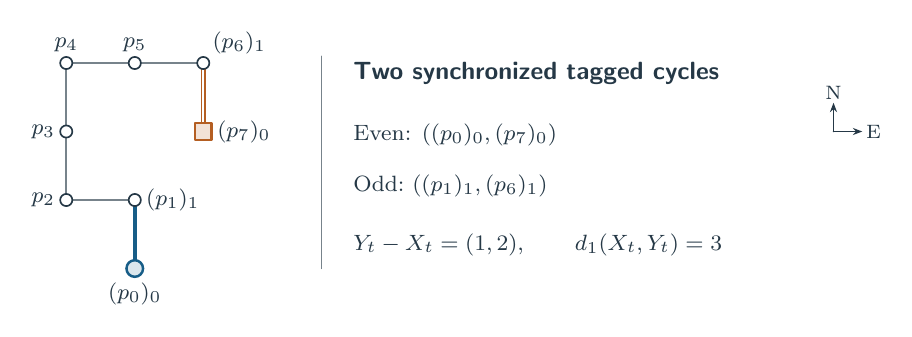
\begin{tikzpicture}[maze,x=8.7mm,y=8.7mm]
 \coordinate (p0) at (1,0); \coordinate (p1) at (1,1);
 \coordinate (p2) at (0,1); \coordinate (p3) at (0,2);
 \coordinate (p4) at (0,3); \coordinate (p5) at (1,3);
 \coordinate (p6) at (2,3); \coordinate (p7) at (2,2);
 \draw[quiet] (p1)--(p2)--(p3)--(p4)--(p5)--(p6);
 \draw[supportA] (p0)--(p1); \draw[supportB] (p7)--(p6);
 \node[startA,label=below:{$(p_0)_0$}] at (p0) {};
 \node[cell,label=right:{$(p_1)_1$}] at (p1) {};
 \node[cell,label=left:{$p_2$}] at (p2) {};
 \node[cell,label=left:{$p_3$}] at (p3) {};
 \node[cell,label=above:{$p_4$}] at (p4) {};
 \node[cell,label=above:{$p_5$}] at (p5) {};
 \node[cell,label=above right:{$(p_6)_1$}] at (p6) {};
 \node[startB,label=right:{$(p_7)_0$}] at (p7) {};
 \node[paneltitle] at (4.05,2.85) {Two synchronized tagged cycles};
 \node[note] at (4.05,1.95) {Even: $((p_0)_0,(p_7)_0)$};
 \node[note] at (4.05,1.20) {Odd:\ $((p_1)_1,(p_6)_1)$};
 \node[note] at (4.05,.35) {$Y_t-X_t=(1,2),\qquad d_1(X_t,Y_t)=3$};
 \draw[rvMid,line width=.4pt] (3.72,.0)--(3.72,3.1);
 \mazeCompass{11.2}{2.0}
\end{tikzpicture}
\caption{The eight-cell path obstruction under the two W9 rows in \eqref{eq:p8-w9-rows}. The circle and square mark state-$0$ starts; both phases have the same displacement $(1,2)$.}
\label{fig:path-p8}
\end{figure}


If a controller with at most two states already has a path trap through seven cells, the desired upper bound is immediate.  A one-state controller has a four-cell path trap by Corollary~\ref{cor:one-state-radius-one}.  Otherwise a genuine two-state path survivor satisfies the W9 consequence after simultaneous compass transport, and the inverse symmetry carries the displayed eight-cell trap back to the original controller.  Hence
\[
 F_{\mathcal P,1}(2)\le8.
\]

\subsection{Exact finite lower certificate}

For the reverse inequality, use the two-state controller in Table~\ref{tab:path-survivor}.

\begin{table}[!htbp]
\centering\small
\begin{tabular}{@{}c|cc@{}}
\toprule
Mask & state $0$ & state $1$\\
\midrule
$\N$ & $(\N,1)$ & $(\N,0)$\\
$\E$ & $(\E,1)$ & $(\E,0)$\\
$\Sdir$ & $(\Sdir,0)$ & $(\Sdir,0)$\\
$\W$ & $(\W,0)$ & $(\W,1)$\\
$\N\Sdir$ & $(\Sdir,0)$ & $(\N,1)$\\
$\E\W$ & $(\W,0)$ & $(\E,1)$\\
$\N\E$ & $(\E,1)$ & $(\N,1)$\\
$\E\Sdir$ & $(\Sdir,0)$ & $(\E,1)$\\
$\N\W$ & $(\W,0)$ & $(\N,1)$\\
$\Sdir\W$ & $(\Sdir,0)$ & $(\Sdir,0)$\\
\bottomrule
\end{tabular}
\caption{The two-state controller used in the exact finite lower certificate for paths.  Rows of degree three and four may be completed arbitrarily because they are never queried on a path.}
\label{tab:path-survivor}
\end{table}


\begin{proposition}[Finite path-survival certificate]\label{prop:path-seven-survivor}
The controller of Table~\ref{tab:path-survivor} succeeds from every state-zero start pair on every induced grid path with at most seven cells.
\end{proposition}

\paragraph{Exact verification.}
The proof is computational and exhaustive.  Paths are enumerated up to translation only, so absolute compass orientation is retained.  The numbers of path shapes on $1,\ldots,7$ cells are
\[
 1,\ 2,\ 6,\ 14,\ 34,\ 82,\ 198,
\]
for a total of $337$.  Across those paths there are exactly $4042$ unordered start pairs whose initial Manhattan distance exceeds one.  For each pair, the deterministic product trajectory is followed until either distance-one contact occurs or a complete product tag repeats.  A repeated product tag before contact is an exact infinite-failure certificate, so no time cutoff is used.  All $4042$ pairs succeed.  An independently written connected-cell-set generator reproduces the same path sets through seven cells.  The checker, data, and enumeration specification belong to the computational supplement.

Proposition~\ref{prop:path-seven-survivor} gives $F_{\mathcal P,1}(2)>7$.  Together with the analytic upper bound it proves Theorem~\ref{thm:path-two-state} with the stated mixed status.

\subsection{Four states solve every finite path}

The behavior changes qualitatively by four states.  Let
\[
 Q=\{\N,\E,\Sdir,\W\}
\]
with any one label, say $\N$, designated as the initial state.  Fix the cyclic order
\[
 \N,\E,\Sdir,\W.
\]
For a nonempty mask $M$ and state $q$, let $\operatorname{succ}_M(q)$ be the first member of $M$ encountered strictly after $q$ in this cyclic order, wrapping around if necessary.  Define
\begin{equation}\label{eq:four-state-rotor}
 d=\operatorname{succ}_M(q),
 \qquad
 \delta(q,M)=(d,-d).
\end{equation}
After the first move, the state records the compass port leading back to the cell just left; the next move takes the next open port in cyclic order.

\begin{proposition}[Contour recurrence on grid trees]\label{prop:four-state-contour}
On every finite induced grid tree $T$ with at least two cells, the controller \eqref{eq:four-state-rotor} has one recurrent cycle on the arrival-port tags
\[
 H=\{(v,q):q\in M_T(v)\}.
\]
This cycle has length $2|E(T)|$ and traverses every directed tree edge exactly once.  Every tag outside $H$ enters $H$ after one step.
\end{proposition}
\begin{proof}
If the controller moves from $v$ in direction $d$, then at the new cell the state is $-d$, the port leading back to $v$.  Hence every transition lands in $H$.

Restricted to $H$, the map takes an incoming port to the next incident port in the fixed cyclic order.  It is a permutation: for an arrival tag $(v,q)$, the previous cell must be $u=v+q$; choosing at $u$ the incident port immediately preceding $-q$ makes the next selected direction equal to $-q$, which lands at $(v,q)$.

To prove that this permutation has one cycle, induct on the number of edges.  A single edge gives the two-tag shuttle.  If $z$ is a leaf adjacent to $v$, remove $z$.  By induction the smaller tree has one contour cycle.  Restoring the leaf inserts its incident port into the cyclic order at $v$: one old successor transition is replaced by the detour $v\to z\to v$ followed by the formerly chosen next edge.  Thus the two directed tags of the restored edge are inserted into, rather than separated from, the existing cycle.  Repeating this leaf insertion yields one cycle on all of $H$.  Finally
\[
 |H|=\sum_{v\in V(T)}\deg_T(v)=2|E(T)|.
\]
\end{proof}

This proposition is a contour statement, not a rendezvous theorem on branching trees.  On a path, however, the contour support is itself a path, so Section~\ref{sec:support-structure} applies directly.

\begin{theorem}[Universal four-state path controller]\label{thm:four-state-path}
The controller \eqref{eq:four-state-rotor} succeeds from every start pair on every finite induced grid path at radius one.
\end{theorem}
\begin{proof}
A singleton succeeds at time zero.  On any nonsingleton path, Proposition~\ref{prop:four-state-contour} puts every trajectory on the same recurrent tagged cycle after at most one move.  Its spatial support is the whole path.  The two trajectories are therefore phase shifts of one periodic path walk, and Corollary~\ref{cor:same-cycle-path-contact} forces distance-one contact.
\end{proof}

\begin{corollary}[Infinite path threshold from four states onward]\label{cor:path-infinity}
For every real $\rho\ge1$ and every $s\ge4$,
\[
 \boxed{F_{\mathcal P,\rho}(s)=\infty.}
\]
\end{corollary}
\begin{proof}
The one fixed controller in Theorem~\ref{thm:four-state-path} has no finite path trap at radius one, and hence none at any larger radius.  It is admissible under every budget $s\ge4$.  Equation~\eqref{eq:F-infinity-meaning} gives the conclusion.
\end{proof}

The remaining path transition is exactly the three-state case:
\[
 F_{\mathcal P,1}(1)=4,\qquad
 F_{\mathcal P,1}(2)=8,\qquad
 F_{\mathcal P,1}(3)\ \text{is undetermined},\qquad
 F_{\mathcal P,1}(s)=\infty\ (s\ge4).
\]
The branching counterexample in Appendix~\ref{app:branching-example} explains why the two-state path-support mechanism does not extend automatically once three states are available; it does not settle the three-state path problem.

\section{Three-state recurrent-cycle realization}\label{sec:realization}

A recurrent word must satisfy both capacity and shared-table compatibility.
We characterize the latter on three-state paths; initial-state accessibility remains
a separate question. Figure~\ref{fig:realization-pipeline} previews the construction.

\subsection{The normal form and its scope}

\begin{proposition}[Three-state path normal form]\label{prop:three-normal-form}
Let a simple three-state tagged cycle have used path support with $n\ge3$ vertices.
Every edge multiplicity is one or two; the doubled edges form a matching.
Up to cyclic shift its spatial word is the ordinary contour, with one passage of
each doubled edge replaced by the three-step passage ``forward, back, forward.''
The choice of the forward or backward contour passage is its insertion phase.
\end{proposition}
\begin{proof}
For adjacent edges, capacity gives $k_{j-1}+k_j\le3$ and both multiplicities are
positive. Hence every $k_j$ is one or two, and two doubled edges cannot be adjacent.
A neighbouring single edge is crossed once in each direction. The additional two
crossings of a doubled edge must therefore lie within one of its two contour
passages; otherwise a neighbouring single-edge cut would be crossed again.
They form the stated immediate backtrack. Endpoint insertions can have equivalent
cyclic descriptions, so uniqueness of the parametrization is not asserted.
\end{proof}

For a one-edge support the multiplicity can instead be three; that case is not a
matching input and is treated separately in Lemma~\ref{lem:one-edge-realization}.
The normal-form necessity concerns used support and remains valid in a larger maze.
The converse below uses the masks of the path itself. A proper interval of an ambient
path requires the boundary-aware conditions in Appendix~\ref{app:boundary-aware}.

Fix a finite induced grid path $P=(v_0,\ldots,v_{n-1})$, $n\ge2$, with its absolute
compass orientation and exactly its own masks. Choose a matching
$\mathcal D_2\subseteq\{0,\ldots,n-2\}$ and phases $\eta_e\in\{0,1\}$.
In the contour $0,1,\ldots,n-1,n-2,\ldots,1$, replace the index-increasing passage
of $e$ if $\eta_e=0$, and its index-decreasing passage if $\eta_e=1$, by the
three-step backtrack. Denote this specification by $S$, and write
\[
 I=\Z/L\Z,\quad L=2(n-1)+2|\mathcal D_2|,\quad
 w_i\in V(P),\quad \sigma(i)=i+1,\quad M_i=M_P(w_i).
\]
Let $d_i$ be the direction from $w_i$ to $w_{\sigma(i)}$.
An occurrence means an index $i\in I$, not just its cell. Internal cells have load
two or three, and endpoints load one or two. An internal cell of load three is
\emph{saturated}. Realization asks for a legal three-state table and states $q_i$
such that the $L$ distinct tags $(w_i,q_i)$ follow this cyclic word. No primitive
spatial-word hypothesis or state-zero accessibility requirement is imposed.

A necessary local condition is \emph{same-mask doubled-side consistency}: all
saturated cells of one absolute mask must use the same port twice. We call this the
direction condition. The finite profile family and matrices in the next theorem are
constructed explicitly below from masks, occurrences and successor links.

\begin{theorem}[Exact three-state realization]\label{thm:three-state-realization}
For every specification $S$ just defined, the following are equivalent:
\begin{enumerate}[label=(\roman*),leftmargin=2em]
\item $S$ is realized by a simple three-state tagged cycle on the path with its own masks;
\item the direction condition holds and some $\theta\in\Theta(S)$ satisfies
\[
 \rank_{\Ftwo}A_\theta=\rank_{\Ftwo}[A_\theta\mid b_\theta];
\]
\item the direction condition holds and there is \emph{one} $\theta\in\Theta(S)$ such that
\[
 \forall\lambda:\quad\lambda^TA_\theta=0\ \Longrightarrow\ \lambda^Tb_\theta=0.
\]
\end{enumerate}
From a consistent profile and its solution one constructs all $45$ legal controller
rows. The resulting cycle has least tagged period exactly
$L=2(n-1)+2|\mathcal D_2|$. Every realizing state assignment belongs to at least one
profile. The same profile is used throughout all components of the specification.
\end{theorem}

% A diagram of the existing finite-profile construction. All components share theta.
\begin{figure}[tbp]
\centering
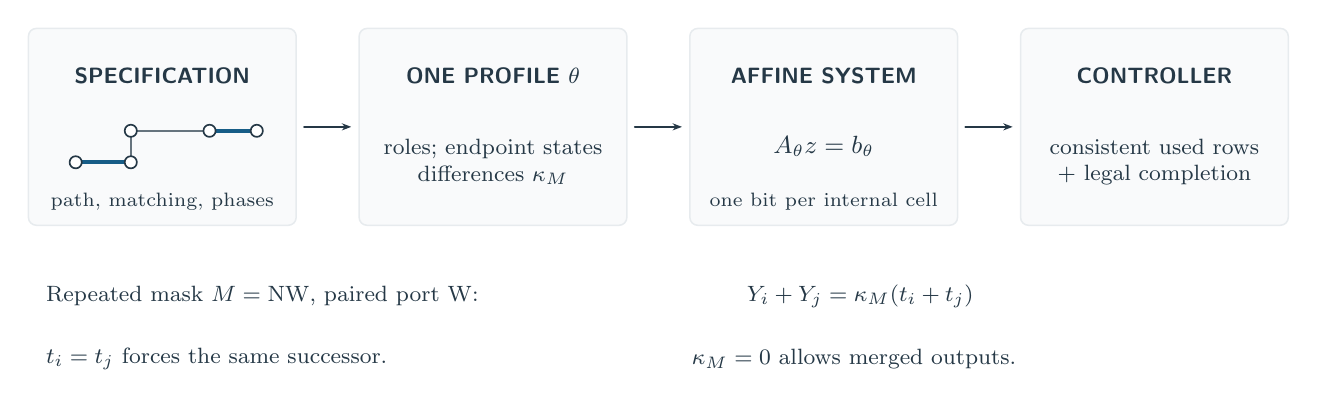
\begin{tikzpicture}[maze,x=1mm,y=1mm]
 \foreach \x in {0,42,84,126}{\draw[lightpanel] (\x,17) rectangle (\x+34,42);}
 \node[font=\footnotesize\sffamily\bfseries,align=center] at (17,36) {SPECIFICATION};
 \draw[edge] (6,25)--(13,25)--(13,29)--(23,29)--(29,29);
 \draw[supportA] (6,25)--(13,25); \draw[supportA] (23,29)--(29,29);
 \foreach \x/\y in {6/25,13/25,13/29,23/29,29/29}{\node[cell] at (\x,\y) {};}
 \node[font=\scriptsize] at (17,20) {path, matching, phases};
 \node[font=\footnotesize\sffamily\bfseries,align=center] at (59,36) {ONE PROFILE $\theta$};
 \node[font=\footnotesize,align=center] at (59,25) {roles; endpoint states\\differences $\kappa_M$};
 \node[font=\footnotesize\sffamily\bfseries,align=center] at (101,36) {AFFINE SYSTEM};
 \node[font=\small] at (101,27) {$A_\theta z=b_\theta$};
 \node[font=\scriptsize] at (101,20) {one bit per internal cell};
 \node[font=\footnotesize\sffamily\bfseries,align=center] at (143,36) {CONTROLLER};
 \node[font=\footnotesize,align=center] at (143,25) {consistent used rows\\+ legal completion};
 \foreach \x in {35,77,119}{\draw[flow] (\x,29.5)--(\x+6,29.5);}
 \node[font=\footnotesize,anchor=west] at (1,8) {Repeated mask $M=\N\W$, paired port $\W$:};
 \node[font=\footnotesize,anchor=west] at (90,8) {$Y_i+Y_j=\kappa_M(t_i+t_j)$};
 \node[font=\footnotesize,anchor=west] at (1,0) {$t_i=t_j$ forces the same successor.};
 \node[font=\footnotesize,anchor=west] at (83,0) {$\kappa_M=0$ allows merged outputs.};
\end{tikzpicture}
\caption{The realization construction, with $Y_i=X_{\sigma(i)}$. The same profile serves every repeated-mask component; varying the profile gives a finite union of affine solution sets, not one XOR system.}
\label{fig:realization-pipeline}
\end{figure}


\subsection{Two-input functionality and the finite profile}

The algebraic mechanism concerns a function on two inputs, not an invertible
successor map. Encode the three states by the nonzero vectors
\[
 H=\Ftwo^2,\qquad Q_3=H\setminus\{0\}=\{1,2,3\},
\]
where the numbers are binary vector codes and addition is XOR. The final controller
names are obtained by $1\mapsto0$, $2\mapsto1$, $3\mapsto2$.

\begin{lemma}[Two-input successor difference]\label{lem:successor-difference}
For input bits $t_i\in\Ftwo$ and output states $Y_i\in Q_3$, the conditions
\[
 t_i=t_j\ \Longrightarrow\ Y_i=Y_j\quad\text{for all }i,j
\]
are equivalent to the existence of $\kappa\in H$ with
\[
 Y_i+Y_j=\kappa(t_i+t_j)\quad\text{for all }i,j.
\]
\end{lemma}
\begin{proof}
If only one input occurs, all outputs coincide and $\kappa=0$ works. If both occur,
functionality gives two outputs $Y_0,Y_1$; take $\kappa=Y_0+Y_1$.
Conversely, equal inputs make the right side zero and force equal outputs.
The case $Y_0=Y_1$ is allowed and is exactly the zero difference.
\end{proof}

For two occurrences of $M=\N\W$ on its paired $\W$-side, take $\kappa=3=(1,1)$ and role bits
$t_i=z_u$, $t_j=z_v$. If the observed successors are $Y_i=1$, $Y_j=2$,
the lemma gives $3=3(z_u+z_v)$, hence $z_u+z_v=1$ over $\Ftwo$.
Equal outputs instead require equal bits for this nonzero difference; $\kappa=0$
allows both inputs to share an output. This is an algebraic illustration, not a
claim that a separately prescribed path is realizable.

Every internal vertex uses both ports. A realizing three-state direction map at its
mask is therefore a surjection with fibres of sizes one and two. For each internal
mask $M$ choose its singleton port $u_M$, its singleton state $a_M\in Q_3$, and let
$p_M$ be the other port. If $M$ has a saturated representative, $p_M$ must be its
doubled port, so $u_M$ is forced; otherwise both port choices are retained.
Choose a successor difference $\kappa_M\in H$, restricted to $\kappa_M\ne0$ when
$M$ is saturated. For each endpoint separately choose an injective assignment of
its actual occurrences to $Q_3$. These choices form $\theta\in\Theta(S)$.
They assign no arbitrary row outputs.

Let $b(a)$ be the smaller numeric code in $Q_3\setminus\{a\}$.
For every internal cell $v$ introduce one bit $z_v$. Define its occurrence states by
\begin{equation}\label{eq:real-roles}
 X_i=\begin{cases}
 a_{M_i},&d_i=u_{M_i},\\
 b(a_{M_i})+a_{M_i}t_i,&d_i=p_{M_i},
 \end{cases}
 \qquad t_i=z_{w_i}+\epsilon_i.
\end{equation}
At a load-two cell the unique paired-side occurrence has $\epsilon_i=0$.
At a saturated cell the two such occurrences have $\epsilon=0,1$ in temporal
order after choosing an origin of the cyclic word. Endpoint $X_i$ are the constants
chosen in the profile. The two paired states are $b(a_M)$ and $b(a_M)+a_M$,
both nonzero and different from $a_M$. Thus local injectivity is built in.
The state absent over a load-two cell is still a possible row state of its mask;
it cannot be discarded globally.

\subsection{The canonical affine system}

For an internal mask form
\[
 U_M=\{i:M_i=M,\ d_i=u_M\},\qquad
 B_M=\{i:M_i=M,\ d_i=p_M\}.
\]
Both groups are nonempty. In each choose an anchor $j$, for example the least
occurrence index. For every other occurrence $i$ impose respectively
\begin{align}
 X_{\sigma(i)}+X_{\sigma(j)}&=0 &&(i,j\in U_M),\label{eq:real-U}\\
 X_{\sigma(i)}+X_{\sigma(j)}&=\kappa_M(t_i+t_j)
 &&(i,j\in B_M).\label{eq:real-B}
\end{align}
Endpoint occurrences are grouped by the \emph{pair} consisting of their one-port
mask and their chosen state. For every non-anchor member of such a group impose
\begin{equation}\label{eq:real-E}
 X_{\sigma(i)}+X_{\sigma(j)}=0.
\end{equation}
In particular, equal endpoint masks cannot be ignored. Equal states at different
masks do not identify rows, and different states at the same endpoint mask are not
identified either.

For a fixed $\theta$, all $a_M$, $\kappa_M$ and endpoint assignments are constants.
Expanding the vector equations into their two scalar coordinates gives
\begin{equation}\label{eq:real-system}
 A_\theta z=b_\theta,\qquad z\in\Ftwo^{n-2}.
\end{equation}
Constant equations are retained: $0=1$ rejects a profile. For $n=2$ there are no
internal bits and the same construction is a zero-dimensional system.

A group of $h$ occurrences contributes $h-1$ vector comparisons. There are fewer
than $2L$ scalar rows, each involving at most two source bits and two successor bits.
The symbolic object consequently has size $O(n)$ and is constructed without solving
realizability. If $m_3$ internal masks have saturated representatives and $m_2$ do
not, then $m_3+m_2\le6$ and
\begin{equation}\label{eq:profile-bound}
 |\Theta(S)|\le36\,9^{m_3}24^{m_2}\le36\,24^6.
\end{equation}
This deliberately coarse constant is independent of the path length. Profiles may
overlap; uniqueness of representation is not required.

\subsection{Proof of the realization theorem}

\begin{proof}[Proof of Theorem~\ref{thm:three-state-realization}]
\emph{Necessity.}
Let a legal table realize the distinct tags. Encode its states in $Q_3$.
At every internal mask both directions occur, so its direction fibres have sizes
one and two. At a saturated cell all three states occur, with the two states on the
doubled side distinct. Therefore every saturated representative of that mask doubles
the same side. Extract $u_M,a_M,p_M$ from the table. At each cell the paired state
or ordered pair determines a bit $z_v$ in \eqref{eq:real-roles}. The endpoint states
give the required injections.

All sources in $U_M$ have the same state and mask; deterministic successor states
give \eqref{eq:real-U}. In $B_M$, source-state equality is equivalent to equality
of $t_i$. Lemma~\ref{lem:successor-difference}, with $Y_i=X_{\sigma(i)}$,
gives a $\kappa_M$ satisfying \eqref{eq:real-B}.
When the mask is saturated, its two paired occurrences at one cell move to the
same neighbour along the doubled edge. Their successor occurrences are distinct,
and distinct tags over that neighbour have different states. Hence their difference
is nonzero, as required in the profile. This also covers a doubled edge incident to
an endpoint. Equal endpoint keys give exactly \eqref{eq:real-E}.
Thus the extracted profile and bits solve \eqref{eq:real-system}; every row
dependency has zero right-hand-side sum.

These comparisons exhaust repeated keys. Different masks mean different rows.
For the same internal mask, singleton and paired states are disjoint, and each
fibre is handled above. A one-port endpoint mask cannot equal a two-port internal
mask. The remaining endpoint coincidences are precisely the groups in
\eqref{eq:real-E}. In particular no additional successor-row condition is missing.

\emph{Linear consistency.}
Row elimination over $\Ftwo$ produces an inconsistent equation exactly when a sum
of original rows has zero left side and right side one. If no such row occurs,
assign the free bits and back-substitute the pivot bits. This proves the equivalence
of rank consistency, the stated balance condition, and existence of a solution,
including the zero-dimensional case.

\emph{Sufficiency and reconstruction.}
Take one consistent profile and a solution. Equations~\eqref{eq:real-roles}
produce nonzero state vectors. At a load-two cell the singleton and paired states
are different. At a saturated cell the opposite $\epsilon$ values produce both
paired states, distinct from each other and from the singleton. Endpoint injections
are part of the profile. Hence all $L$ resulting tags are distinct.

Apply the one global renaming to actual controller states $q_i\in\{0,1,2\}$ and
prescribe every used row by
\begin{equation}\label{eq:real-used-controller}
 \delta(q_i,M_i)=(d_i,q_{\sigma(i)}).
\end{equation}
Suppose two prescriptions have the same key. At an internal mask both sources lie
in the same direction fibre. In the singleton fibre, adding their anchor equations
gives equal successors. In the paired fibre, equal states give $t_i=t_j$, and
adding their anchor equations yields
\[
 X_{\sigma(i)}+X_{\sigma(j)}=\kappa_M(t_i+t_j)=0.
\]
The direction already agrees. At an endpoint the direction is unique, and
\eqref{eq:real-E} gives equal successors for equal keys. Thus
\eqref{eq:real-used-controller} is a function, not a conflicting set of assignments.

Every used direction belongs to its mask. For each still unassigned key $(q,M)$,
$M\ne\varnothing$, choose any $d\in M$ and any next state. This produces all
$3(2^4-1)=45$ legal rows without changing a used row. If only one paired input was
observed, its profile difference need not prescribe the absent row's output.
In particular, one must not extrapolate it to a zero vector and treat that vector
as a state. The observed difference may instead be replaced by zero without
changing the realized assignments.

Starting at $(w_0,q_0)$, the prescribed row takes the controller to
$(w_{\sigma(0)},q_{\sigma(0)})$; induction follows the entire specified word.
In each selected compass direction the next cell is the prescribed neighbour.
The orbit returns after $L$ steps, and the preceding $L$ tags are distinct.
Its least tagged period is therefore exactly $L$. This argument neither assumes
nor needs that the spatial projection have least period $L$.
\end{proof}

The same key comparisons close all successor equalities. Within a fixed profile,
linear elimination tests or projects partial assignments; across profiles, one takes
a union. Unsaturated vertices therefore have no automatic completion rule.

\subsection{Why one XOR system is not enough}

Consider the fixed specification
\[
 \text{directions }\E\N\E\N\N\N\E,\qquad
 \mathcal D_2=\{0,2,6\},\qquad \eta_e=0,
\]
whose masks are $\E,\N\W,\E\Sdir,\N\W,\N\Sdir,\N\Sdir,\E\Sdir,\W$.
Its cyclic word is
\[
 (0,1,0,1,2,3,2,3,4,5,6,7,6,7,6,5,4,3,2,1).
\]
Let $x$ denote the same/swap correspondence of the ordered west-state pairs
$(q_1,q_{19})$ and $(q_5,q_{17})$ at the two saturated $\N\W$ cells.
Let $y$ denote that of the east-state pairs $(q_4,q_6)$ and $(q_{10},q_{12})$
at the two saturated $\E\Sdir$ cells; zero means same and one swap.
The two intervening $\N\Sdir$ cells are unsaturated.

\begin{proposition}[A non-affine saturated correspondence relation]\label{prop:nand8}
For this fixed spatial specification, the exact extendible relation is
\[
 \operatorname{Ext}(x,y)=\{00,01,10\}.
\]
\end{proposition}
\begin{proof}
The singleton $\N\W/\N$ rows give $q_3=q_7$ and $q_4=q_8$.
The singleton $\E\Sdir/\Sdir$ rows give $q_{18}=q_{14}$ and $q_{19}=q_{15}$.
If $x=1$, then $q_{17}=q_1\ne q_{19}$. Equality of the two $\N\Sdir/\Sdir$
source states, $q_{16}=q_{15}$, would force $q_{17}=q_{16}=q_{19}$ by their
successor rows. Thus two different south states are needed. If $y=1$, then
$q_{10}=q_6\ne q_4=q_8$. Equality of the north states $q_8=q_9$ would force
$q_9=q_{10}$, again a contradiction. Hence two different north states are needed.
North and south states at the same mask cannot coincide. The assignment $11$
would therefore need four states. Appendix~\ref{app:nand-witnesses} gives full
realizing state assignments for the other three choices.
\end{proof}

An XOR solution set and its projections are affine, with one, two or four possible
assignments on two bits, never three. Even auxiliary XOR variables therefore cannot
describe these actual correspondences by one system. This excludes faithful
correspondence encodings, not arbitrary hypothetical decision-only graphs. The
insertion phases $\eta_e$ are fixed, distinct from $x,y$; the unpinned specification
is realizable.

\subsection{An infinite phase-locking family}\label{subsec:phase-locking}

\begin{theorem}[Phase locking across arbitrary gaps]\label{thm:phase-locking}
Let $r\ge1$ and $\ell_0,\ldots,\ell_r\ge1$. On the induced monotone path
\[
 \E^{\ell_0}\N\E^{\ell_1}\N\cdots\N\E^{\ell_r},
\]
double all $r$ north edges and no others, assigning phases $\eta_1,\ldots,\eta_r$.
The specification is realizable with three states if and only if all phases are equal.
\end{theorem}
\begin{proof}
The lower endpoint of each doubled north edge has mask $\N\W$ and singleton west
state $w$; the upper endpoint has mask $\E\Sdir$ and singleton east state $e$.
At the $j$th edge denote its temporal north states by $A_j,B_j$ and its south
states by $C_j,D_j$. Then
$\{A_j,B_j,w\}=Q$ and $\{C_j,D_j,e\}=Q$.
For either insertion phase the south rows give
\[
 C_j\longmapsto B_j,\qquad D_j\longmapsto w.
\]
Two pairs $(C_j,D_j)$ and $(C_k,D_k)$ either agree or are swapped.
A swap would identify $B_j$ with $w$, so the pairs agree; then $B_j=B_k$ and
$A_j=A_k$. The north rows are
\[
\begin{array}{c|cc}
\eta_j& A_j & B_j\\\hline
0&C_j&e\\
1&e&D_j
\end{array}
\]
and distinct phases would identify a paired state with the singleton $e$.
Thus all phases are equal, independently of the horizontal gaps.

For sufficiency, use the following rows; the two rows for each phase list the
three outputs in state order $0,1,2$:
\[
\begin{array}{c|ccc}
 (\eta,M)&0&1&2\\\hline
 (0,\N\W)&(\W,2)&(\N,1)&(\N,0)\\
 (0,\E\Sdir)&(\E,1)&(\Sdir,2)&(\Sdir,0)\\
 (1,\N\W)&(\W,2)&(\N,0)&(\N,1)\\
 (1,\E\Sdir)&(\E,1)&(\Sdir,0)&(\Sdir,2)
\end{array}
\]
For either phase add
$\delta(1,\E\W)=(\E,1)$, $\delta(2,\E\W)=(\W,2)$,
$\delta(2,\E)=(\E,1)$, and $\delta(1,\W)=(\W,2)$.
Start at the left endpoint in state $2$. At phase zero the forward doubled-edge
sequence is $\N\W_1,\E\Sdir_1,\N\W_2,\E\Sdir_0$, with backward sequence
$\E\Sdir_2,\N\W_0$. At phase one the forward sequence is
$\N\W_1,\E\Sdir_0$, and the backward sequence is
$\E\Sdir_2,\N\W_2,\E\Sdir_1,\N\W_0$.
Here a mask with a subscript denotes the occurrence at the corresponding endpoint
of that edge with that state. Horizontal segments preserve state $1$ eastward and
state $2$ westward. The endpoint rows close the word; all occurrences at one cell
have different states. Completing unused rows gives the required simple cycle.
\end{proof}

With $r=2$ and all gaps one, unequal phases give the six-vertex staircase.
Its contradiction is equivalently the three constraints $x=1$, $x+y=0$, $y=0$
from the general successor comparisons, whose sum is $0=1$; an explicit derivation
is recorded in Appendix~\ref{app:staircase}. Minimality of six among residual
obstructions is a finite-check statement, not needed for this proof.
More generally, for any fixed path radius $R$, choose gaps $(1,h,1)$ with
$h>2R+2$ and phases $(0,1)$. Every radius-$R$ neighbourhood occurs in a realizable
uniform-phase specification, but the whole specification is unrealizable.
Thus bounded geometric neighbourhoods do not replace the global mask constraints.
This is not a lower bound on the size of an algebraic certificate.

\subsection{Recognition, reconstruction and the accessibility boundary}

Enumerate the finite profiles after checking the direction condition, compile
\eqref{eq:real-system}, and solve by Gaussian elimination. A successful branch
constructs the table by \eqref{eq:real-used-controller}; rejection requires failure
of every admissible profile. With $K$ bounded as in \eqref{eq:profile-bound}, this
gives a coarse $O(Kn^3)$ time bound and $O(n^2)$ working space. Fixed-alphabet
polynomiality is not asserted as a separate novelty: finitely many full tables already
exist independently of $n$. The content is the special sparse normal form and
constructive removal of arbitrary row outputs.

Realization does not determine state-zero accessibility: two completions on one
four-vertex path preserve the same contour while making it accessible from every
state-zero start or from none. Appendix~\ref{app:basins} gives both tables and a
conditional uniqueness criterion. Universal three-state rendezvous remains open.

\section{State-complexity consequences}\label{sec:state-complexity}

Theorem~\ref{thm:FM-duality} converts trap thresholds into memory requirements:
\[
 F_{\mathcal C,\rho}(s)>n
 \quad\Longleftrightarrow\quad
 M_{\mathcal C,\rho}(n)\le s.
\]
The strict inequality on the left is essential.

\subsection{Consequences of the exact low-state thresholds}

For all induced grid mazes at radius one, Section~\ref{sec:memoryless-radius} gives $F(1)=4$, while the central theorem of Section~\ref{sec:two-state} gives $F(2)=7$.  Therefore
\begin{equation}\label{eq:M-original-small}
 \boxed{M(1)=M(2)=M(3)=1},
 \qquad
 \boxed{M(4)=M(5)=M(6)=2},
\end{equation}
and
\begin{equation}\label{eq:M7-bound}
 \boxed{3\le M(7)<\infty}.
\end{equation}
Indeed, $F(1)>n$ exactly for $n\le3$ among these horizons, and $F(2)>n$ exactly for $n\le6$.  The strict lower bound at $n=7$ follows because $F(2)=7$ is not greater than seven; finiteness follows from Theorem~\ref{thm:finite-M} below.

For induced paths, Theorem~\ref{thm:path-two-state} and Corollary~\ref{cor:path-infinity} give the sharper hierarchy
\begin{equation}\label{eq:M-path-small}
 M_{\mathcal P,1}(n)=1\quad(n\le3),
 \qquad
 M_{\mathcal P,1}(n)=2\quad(4\le n\le7),
\end{equation}
and
\begin{equation}\label{eq:M-path-large}
 \boxed{M_{\mathcal P,1}(n)\in\{3,4\}\qquad(n\ge8).}
\end{equation}
The first equality is deductive; the exact value $2$ on $4\le n\le7$ inherits the finite lower certificate of Theorem~\ref{thm:path-two-state}. The two-value alternative \eqref{eq:M-path-large} is deductive: the analytic bound $F_{\mathcal P,1}(2)\le8$ gives $M>2$, and the four-state universal controller gives $M\le4$.

\begin{table}[!htbp]
\centering\small
\begin{tabular}{@{}c|c|c@{}}
\toprule
Size horizon & all induced grid mazes, $M(n)$ & induced paths, $M_{\mathcal P,1}(n)$\\
\midrule
$1\le n\le3$ & $1$ & $1$\\
$4\le n\le6$ & $2$ & $2$\\
$n=7$ & $3\le M(7)<\infty$ & $2$\\
$n\ge8$ & $3\le M(n)<\infty$; exact value open & $3$ or $4$\\
\bottomrule
\end{tabular}
\caption{State-complexity consequences of the exact obstruction thresholds and the finite-horizon existence theorem.  The last path entry is an exact two-value alternative, not an estimate.}
\label{tab:state-complexity}
\end{table}


The unresolved three-state path problem has an exact dual interpretation.  If a three-state controller succeeds on every finite induced path, then $M_{\mathcal P,1}(n)=3$ for every $n\ge8$.  If no such controller exists, then the finite set of three-state tables has a finite maximum first-trap size $F_{\mathcal P,1}(3)$, and Theorem~\ref{thm:FM-duality} implies $M_{\mathcal P,1}(n)=4$ for all sufficiently large $n$.  Thus deciding universal three-state path rendezvous is equivalent to deciding whether the eventual path state complexity is three or four.

\subsection{Finite state complexity at every fixed horizon}

The upper bound in \eqref{eq:M7-bound} is a general finite-horizon fact.  It must not be confused with a single finite controller that solves mazes of all sizes.

\begin{theorem}[Finite-horizon solvability]\label{thm:finite-M}
For every fixed finite $n$ and every $\rho\ge1$,
\[
 \boxed{M_{\mathcal G,\rho}(n)<\infty.}
\]
The controller may depend on $n$ but not on the maze or the starting cell.
\end{theorem}
\begin{proof}
Fix $n$. Store a bounded exploration record: visited coordinates relative to the
start, their observed masks, the current relative coordinate, a DFS stack and a
mode flag. Coordinates are updated internally from chosen compass moves, not read
from the environment. Since every cell is within graph distance $n-1$ of the start,
they lie in $[-(n-1),n-1]^2$. The finite collection of possible records is a finite
state set.

At each cell, move to the first unvisited neighbour in a fixed compass order and
push the current coordinate onto the stack; when none remains, traverse the stack
edge to the parent. Read a newly reached cell's mask on the transition that chooses
its next move. Thus DFS needs no stationary processing step and eventually returns
to the root with the complete relative map.

Choose the lexicographically largest mapped cell and its first open neighbour in
fixed compass order. Maps from different starts differ by translation, which
preserves both choices; both agents therefore select the same physical edge.
Follow a stored route to its selected endpoint, then shuttle on that edge forever.
The mode change takes the first route edge, or the selected edge itself when already
at the endpoint, so every transition moves. Once both agents shuttle, their
Manhattan distance is zero or one, proving success for every $\rho\ge1$.

A singleton succeeds at time zero. Complete impossible-record rows by arbitrary
legal moves. The resulting table depends on $n$, not on the maze or either start.
\end{proof}

The radius restriction in Theorem~\ref{thm:finite-M} is genuine for this model: when $0\le\rho<1$, opposite starts on a two-cell edge swap forever under compulsory synchronous motion, independently of the number of states.

The next two sections fix first a complete test menu and then one host for all
two-state controllers, strengthening the obstruction quantifiers in the same model.

\section{Finite obstruction bases}
\label{sec:finite-obstructions-universal}

The two-state case proof supplies three levels of obstruction uniformity:
\begin{equation}
\label{eq:three-obstruction-quantifiers}
\begin{aligned}
  &\text{controller-dependent trap complexity:}
  &&\forall A\;\exists I_A,\\
  &\text{finite complete test family:}
  &&\exists\mathcal U\text{ finite}\;\forall A\;\exists I\in\mathcal U,\\
  &\text{one universal host maze:}
  &&\exists U\;\forall A\;\exists(x_A,y_A)\in U^2.
\end{aligned}
\end{equation}
Here $A$ ranges over legal controllers with at most two states, and each test
or start pair is initially noncontacting. The successive lines fix the controller,
then a menu, then the host itself. Finite controller space already gives an abstract
finite menu from $F(2)<\infty$; the construction below instead extracts a small
explicit family from the proof without enumerating controllers.

\subsection{An explicit proof-derived obstruction basis}
\label{subsec:human-obstruction-basis}

A \emph{test instance} is a triple $I=(V,x_0,y_0)$ consisting of an absolutely
oriented finite connected induced grid maze and two distinct state-$0$ starts with
$\|x_0-y_0\|_1\ge2$.  We say that $I$ \emph{traps} $A$ when the two synchronous
copies of $A$ started at $x_0,y_0$ never reach Manhattan distance at most one.
Compass orientation is part of the instance.

\begin{theorem}[Explicit finite obstruction basis]
\label{thm:human-finite-basis}
There is an explicit family $\mathcal U_{\mathrm{hum}}$ of $144$ absolutely oriented,
start-labelled test instances, each on at most seven cells, such that every legal
deterministic controller with at most two states is trapped by at least one member of
$\mathcal U_{\mathrm{hum}}$.

The family uses $76$ fixed oriented maze geometries.  Under simultaneous $D_4$
transport and exchange of the two identical agents it has $22$ instance orbits, and
its maze geometries have $13$ $D_4$-types.
\end{theorem}

\begin{proof}
The upper proof has $30$ primitive terminal predicates.  Making explicit the
two equal-direction variants and the four reset-bit variants produces $34$ normalized
source records.  In every branch the proof applies one global element $g\in D_4$ to
the controller, masks, directions, maze and starts; it never rotates only the maze.
The selected normalized trap is therefore transported back by $g^{-1}$.  We take all
eight inverse transports of all $34$ source records, then quotient only by common
translation, exchange of the two identical state-$0$ agents, and literal identity.
Rotation and reflection are \emph{not} quotient operations on the concrete family,
because the compass is absolute.  This yields exactly the $144$ instances stated
above.

The completeness implication itself is the original case tree.  For an
arbitrary two-state controller that tree reaches one of its terminal source records;
the corresponding normalized execution is trapped by the terminal lemma.  Simultaneous
$D_4$ conjugacy preserves tagged executions and Manhattan distance, so the inverse
transport traps the original controller.  That transported instance belongs to
$\mathcal U_{\mathrm{hum}}$.  A one-state controller is included by viewing it as a
two-state table whose state-$0$ rows always return state $0$.
\end{proof}

The counting in Theorem~\ref{thm:human-finite-basis} is finite bookkeeping rather
than a premise of completeness.  The $34$ normalized source records and all $144$
transported instances are supplied in the supplementary data.  Their terminal
conditions organize into the eight proof modules summarized in
Table~\ref{tab:obstruction-modules}.

% Exact selector summary. Full terminal proofs stay in section 5 and appendix A.
\begin{table}[!htbp]
\centering\small
\setlength{\tabcolsep}{4pt}
\renewcommand{\arraystretch}{1.08}
\begin{tabularx}{\linewidth}{@{}lP{.44\linewidth}Y@{}}
\toprule
Module & Regime / first failed condition & Geometry and noncontact mechanism \\
\midrule
$\mathrm{AX}$ & Straight directions coincide, or a normalized opposed-direction toggle/reset/endpoint test fails.
& Line or U-path, $\le7$ cells. Terminal shuttles or disjoint line supports; parity covers adjacent supports. \\
\addlinespace[3pt]
$\mathrm{RP}$ & After the front tests, both axes reset: $C_i,C_j\in\{C_0,C_1\}$.
& Two three-edge arms, $7$ cells. Closed pockets leave the shared corner unvisited. \\
\addlinespace[3pt]
$\mathrm Z$ & One axis is $C_0$, the other $I$; exchange axes if needed. Six successive corner alternatives.
& L/U/offset path, $\le7$ cells. Closed arm regions or forced prefixes; separation or parity. \\
\addlinespace[3pt]
$\mathrm O$ & One axis is $C_1$, the other $I$. Seven successive corner alternatives.
& L/U/offset path, $\le7$ cells. Closed pockets and forced corner prefixes; separation or parity. \\
\addlinespace[3pt]
$\mathrm{LOCK}$ & Both axes are $I$. After drift/diagonal normalization, the first of three corner-direction tests fails.
& Paired terminal-arm path, $\le7$ cells. Locked disjoint translated supports. \\
\addlinespace[3pt]
$\mathrm{BIT}$ & All three direction tests pass; the first of four required corner output bits fails.
& Six-cell path. Closed tagged regions or a prefix into disjoint cycles; gap or parity. \\
\addlinespace[3pt]
$\mathrm{TAIL}$ & Lock and bit tests pass, but the final two W9 entries do not both hold.
& Seven-cell path. A forced shuttle versus a separated left region, including the transient. \\
\addlinespace[3pt]
$\mathrm J$ & W9 holds. For $u=\delta(0,NSW)$, $v=\delta(1,NSW)$, choose G2 if $v=(S,0)$ or $[u=(S,0),\ v\in\{(N,0),(W,1)\}]$; otherwise G1.
& Seven-cell one-junction tree. Exact tagged words separate the executions through the transient. \\
\bottomrule
\end{tabularx}
\caption{The eight terminal modules: $C_0,C_1$ are reset next-state maps and $I$ is identity. These selectors guide the complete terminal proofs; only $\mathrm J$ needs a junction rather than a path.}
\label{tab:obstruction-modules}
\end{table}


\subsection{A computer-minimized subfamily}
\label{subsec:44-subfamily}

The proof-derived family is intentionally faithful to the proof rather than optimized for
cardinality.  Exact computation gives a smaller complete menu, but its scope must be
stated carefully.

\begin{proposition}[Minimum within the proof-derived candidate family]
\label{prop:44-candidate-minimum}
There exists a complete test family of $44$ instances, all chosen from
$\mathcal U_{\mathrm{hum}}$.  Moreover, no complete subfamily of
$\mathcal U_{\mathrm{hum}}$ has fewer than $44$ members.
\end{proposition}

The existence and candidate-restricted optimum in this proposition are
computer-assisted results, unlike the deductive completeness of the full family.
\paragraph{Certificate sketch.}
For the upper bound, the full physical transition function of each of the $144$
instances was reconstructed, and a SAT encoding of a legal controller escaping the
selected $44$ instances was proved unsatisfiable by an independently checked LRAT
certificate.  For the lower bound, there are $44$ explicit legal controllers
$P_1,\ldots,P_{44}$.  If
\[
  S_i=\{I\in\mathcal U_{\mathrm{hum}}: I\text{ traps }P_i\},
\]
then each $S_i$ is nonempty and the $44$ sets are pairwise disjoint.  Any complete
subfamily of the $144$ candidates must therefore choose a distinct member from each
$S_i$.  This packing argument is a direct exact finite check of the full physical
instances and does not use SAT.

The $44$ tests are complete, but optimality is \emph{restricted to the $144$
supplied candidates}. Whether an arbitrary complete family can have at most $43$
members remains open.

\section{A universal host maze}\label{sec:universal-host}
\label{subsec:universal-host-construction}

Joining traps can change a queried compass mask even when the new edge was never
traversed. A universal induced maze therefore requires protection of the entire
execution, not just its recurrent edges.

A five-cell path already shows the issue.  Number a vertical path $0,1,2,3,4$ from
bottom to top and start the agents at $0$ and $4$.  There are legal completions with
straight-axis rows for which the complete spatial words are
\[
  (0,1,2,1)^\infty,
  \qquad
  (4,3)^\infty.
\]
The distances are $4,2,2,2$ and then repeat, but every old cell is visited.  Any proper
connected induced extension changes the mask of some visited old cell.  Thus one
cannot demand that each original trap already contain a clean attachment site.

\subsection{Clean attachment}
\label{subsubsec:clean-attachment}

\begin{lemma}[Clean attachment]
\label{lem:clean-attachment}
Let $V$ be an induced grid maze and let
\[
  (x_t,q_t,y_t,r_t)_{t\ge0}
\]
be a complete trapped execution in $V$.  Put
\[
  R=\{x_t:t\ge0\}\cup\{y_t:t\ge0\}.
\]
Let $C$ be a finite set of new cells, disjoint from $V$, such that the induced extension
$V'=V\cup C$ is a maze and
\[
  \operatorname{dist}_1(C,R)\ge2.
\]
Then the tagged execution from the same starts is identical in $V$ and $V'$.
In particular the extension introduces no rendezvous.
\end{lemma}

\begin{proof}
Induct on time.  Suppose that both tagged positions agree through time $t$.  Each
current cell belongs to $R$, and no new cell is a grid neighbor of it.  Its complete
compass mask is therefore unchanged.  The controller queries the same row, returns the
same direction and next state, and the selected old neighbor is still present.  Hence
both next tagged positions agree.  The conclusion follows simultaneously for the two
agents.
\end{proof}

The set $R$ must include transient visits. New edges at unvisited old cells are
harmless: the lemma protects queried masks, not every old mask.

\begin{figure}[t]
\centering
% Schematic only. R and its grid distance-one halo are generated explicitly.
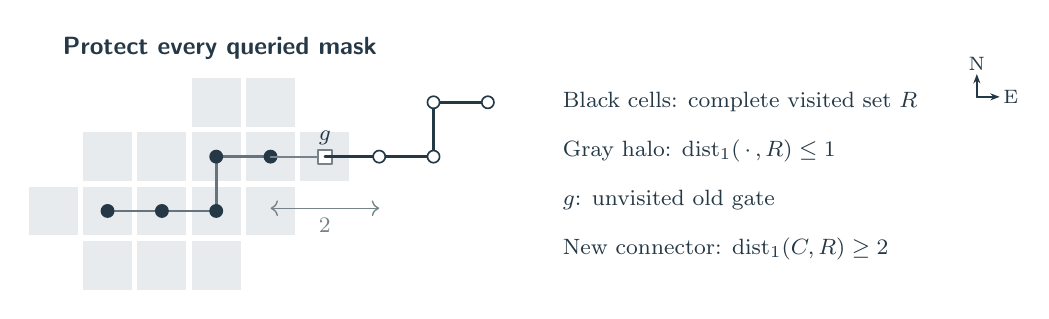
\begin{tikzpicture}[maze,x=6.9mm,y=6.9mm]
 \path[protected] (-1.46,-0.46) rectangle (-0.54,0.46);
 \path[protected] (-0.46,-1.46) rectangle (0.46,-0.54);
 \path[protected] (-0.46,-0.46) rectangle (0.46,0.46);
 \path[protected] (-0.46,0.54) rectangle (0.46,1.46);
 \path[protected] (0.54,-1.46) rectangle (1.46,-0.54);
 \path[protected] (0.54,-0.46) rectangle (1.46,0.46);
 \path[protected] (0.54,0.54) rectangle (1.46,1.46);
 \path[protected] (1.54,-1.46) rectangle (2.46,-0.54);
 \path[protected] (1.54,-0.46) rectangle (2.46,0.46);
 \path[protected] (1.54,0.54) rectangle (2.46,1.46);
 \path[protected] (1.54,1.54) rectangle (2.46,2.46);
 \path[protected] (2.54,-0.46) rectangle (3.46,0.46);
 \path[protected] (2.54,0.54) rectangle (3.46,1.46);
 \path[protected] (2.54,1.54) rectangle (3.46,2.46);
 \path[protected] (3.54,0.54) rectangle (4.46,1.46);
 \draw[edge,line width=1.05pt] (0,0)--(1,0)--(2,0)--(2,1)--(3,1);
 \foreach \x/\y in {0/0,1/0,2/0,2/1,3/1}{\node[cell,fill=rvInk] at (\x,\y) {};}
 \draw[quiet] (3,1)--(4,1);
 \node[gate,label=above:{$g$}] at (4,1) {};
 \draw[rvInk,line width=.9pt] (4,1)--(5,1)--(6,1)--(6,2)--(7,2);
 \foreach \x/\y in {5/1,6/1,6/2,7/2}{\node[cell] at (\x,\y) {};}
 \draw[<->,rvMid,line width=.5pt] (3,.05)--(5,.05) node[midway,below,font=\footnotesize] {$2$};
 \node[paneltitle] at (-1.0,3.0) {Protect every queried mask};
 \node[note] at (8.2,2.0) {Black cells: complete visited set $R$};
 \node[note] at (8.2,1.1) {Gray halo: $\operatorname{dist}_1(\,\cdot\,,R)\le1$};
 \node[note] at (8.2,.2) {$g$: unvisited old gate};
 \node[note] at (8.2,-.7) {New connector: $\operatorname{dist}_1(C,R)\ge2$};
 \mazeCompass{16.0}{2.1}
\end{tikzpicture}

\caption{Clean attachment: the gray distance-one halo protects every cell in the complete
visited set $R$. The new connector meets only an unvisited old gate and stays outside
the halo; the drawing illustrates the clearance condition, not a particular trap.}
\label{fig:clean-attachment}
\end{figure}

\subsection{Unused-cut stretching}
\label{subsubsec:unused-cut-stretching}

The five-cell example above still has an unused edge cut.  Stretching such a cut makes
room for a protected port without modifying the masks of the old cells.

\begin{lemma}[Unused-cut stretching]
\label{lem:unused-cut-stretching}
Let the vertical cut $x=k+\tfrac12$ cross at least one edge of an induced grid maze
$V$, and suppose that neither complete trapped trajectory ever traverses an edge that
crosses this cut.  Define
\[
\phi(x,y)=
\begin{cases}
(x,y),&x\le k,\\
(x+4,y),&x\ge k+1.
\end{cases}
\]
For every old crossing edge $(k,y)(k+1,y)$ insert the four cells
\[
 (k+1,y),(k+2,y),(k+3,y),(k+4,y)
\]
between its image endpoints $(k,y)$ and $(k+5,y)$.  Then every old image cell has
exactly its original compass mask, every actually selected move of the trapped
execution joins the images of the same two old cells, and Manhattan distances between
old image cells do not decrease.  Moreover every inserted cell in the middle column
$x=k+2$ has Manhattan distance at least two from every old image cell.
\end{lemma}

\begin{proof}
Within either half-plane, $\phi$ is a translation, so noncrossing adjacencies and
compass directions are unchanged.  At a crossing edge the left endpoint still has an
east neighbor and the right endpoint still has a west neighbor, now through the
inserted straight corridor; no inserted cell is adjacent to any other old image.
Thus every old mask is exactly preserved.

Mask preservation would not by itself preserve an execution that actually used a
crossing edge, because such a move would enter a new corridor cell.  The unused-cut
hypothesis excludes this: every selected old edge lies wholly in one half-plane and
therefore maps to the same old adjacency.  Induction on time transports the entire
tagged execution.

Distances on one side are unchanged.  For points on opposite sides the horizontal
separation increases by four, so Manhattan distance cannot decrease.  Finally, old
left images have $x\le k$ and old right images have $x\ge k+5$; a cell with $x=k+2$
is therefore at horizontal distance at least $2$ from the former and at least $3$
from the latter.  This is the protected lane required for Lemma~\ref{lem:clean-attachment}.
\end{proof}

The horizontal version is obtained by writing the same geometric construction with
$x$ and $y$ interchanged.  This is a statement about the embedding of a fixed execution;
it does \emph{not} rotate or reflect the fixed controller.

For the cuts used below exactly one old tree edge crosses the cut.  The replacement
therefore subdivides that edge, and a simple route from the protected middle lane to an
external port preserves the tree property and maximum degree three.

\begin{figure}[t]
\centering
% Exact local grid scale, with the cut and its image distinguished.
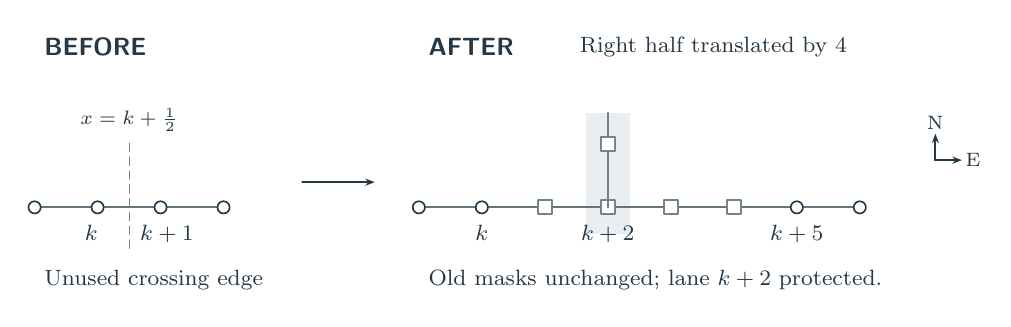
\begin{tikzpicture}[maze,x=8mm,y=8mm]
 \begin{scope}
  \node[paneltitle] at (-1,2.55) {BEFORE};
  \draw[edge] (-1,0)--(0,0)--(1,0)--(2,0);
  \foreach \x in {-1,0,1,2}{\node[cell] at (\x,0) {};}
  \draw[rvMid,densely dashed] (.5,-.65)--(.5,1.05);
  \node[font=\scriptsize,above] at (.5,1.05) {$x=k+\tfrac12$};
  \node[font=\footnotesize,below] at (-.1,-.12) {$k$};
  \node[font=\footnotesize,below] at (1.1,-.12) {$k+1$};
  \node[note] at (-1,-1.15) {Unused crossing edge};
 \end{scope}
 \draw[flow,line width=.8pt] (3.25,.4)--(4.4,.4);
 \begin{scope}[shift={(6.1,0)}]
  \node[paneltitle] at (-1,2.55) {AFTER};
  \node[note] at (1.4,2.55) {Right half translated by $4$};
  \fill[rvGray!85] (1.65,-.43) rectangle (2.35,1.5);
  \draw[edge] (-1,0)--(0,0)--(5,0)--(6,0);
  \foreach \x in {-1,0,5,6}{\node[cell] at (\x,0) {};}
  \foreach \x in {1,2,3,4}{\node[gate] at (\x,0) {};}
  \draw[quiet] (2,0)--(2,1.5); \node[gate] at (2,1) {};
  \node[font=\footnotesize,below] at (0,-.12) {$k$};
  \node[font=\footnotesize,below] at (2,-.12) {$k+2$};
  \node[font=\footnotesize,below] at (5,-.12) {$k+5$};
  \node[note] at (-1,-1.15) {Old masks unchanged; lane $k+2$ protected.};
 \end{scope}
 \mazeCompass{13.3}{.75}
\end{tikzpicture}

\caption{An unused crossing edge before and after width-four stretching. Four inserted
cells preserve the old endpoint masks; the lane $x=k+2$ has clearance for a protected
branch.}
\label{fig:cut-stretching}
\end{figure}

\subsection{Portability of the junction leaves}
\label{subsubsec:junction-portability}

All nonjunction leaves of the case tree are paths and admit an explicitly proved
unused cut through an edge not traversed by either complete execution.  The two final
junction leaves require separate arguments.

For G2, the W9 symbolic words confine one execution to the cells $B,J,A,U$ while the
other alternates on its separated two-cycle; the boundary cell $V$ is never visited.
Its outward ray is therefore a clean port.  For G1, one execution is the fixed word
\[
 B^0,D^1,F^1,D^1,F^1,\ldots
\]
and neither visits $V$ nor traverses $JB$.  The other begins $A^0,J^1$.  The G1 proof
implies the dichotomy
\[
  V\text{ is never visited}
  \qquad\text{or}\qquad
  JB\text{ is never traversed by either execution}.
\]
Indeed, a first visit to $B$ can occur only as $B^1$ and immediately repeats the
already visited tagged state $J^1$, while a visit to $V$ enters the permanent
$U^1,V^1$ two-cycle.  The same execution therefore cannot visit both $B$ and $V$.
In the first alternative we use the clean outward ray of $V$; in the second we stretch
the unused cut through $JB$.  Both G1 variants are included in the fixed host in
advance.  The choice of which one supplies the witness may depend on the controller.

\subsection{Assembly of the universal tree}
\label{subsubsec:universal-tree-assembly}

Applying these port constructions to the inverse compass transports required by the
case tree gives $172$ ported fragments: $156$ unused-cut fragments and $16$
clean-boundary fragments.  The number exceeds $144$ because one oriented test can
have more than one relevant proof provenance or attachment method, and G1 requires
both of its portable alternatives in advance.

Place the $172$ fragment boxes from left to right with two empty columns between
successive boxes.  Extend each exposed port by a vertical stalk to one top horizontal
rail, and join the stalks along that rail.  The separation prevents unintended induced
adjacencies between fragments or stalks, while each fragment has exactly one connection
to the global rail.  The local pieces are trees of maximum degree three, the stalks are
paths, and the rail joins them without cycles.  The induced union is therefore a
subcubic tree.

\begin{figure}[t]
\centering
% A schematic assembly, not the complete 5212-cell coordinate drawing.
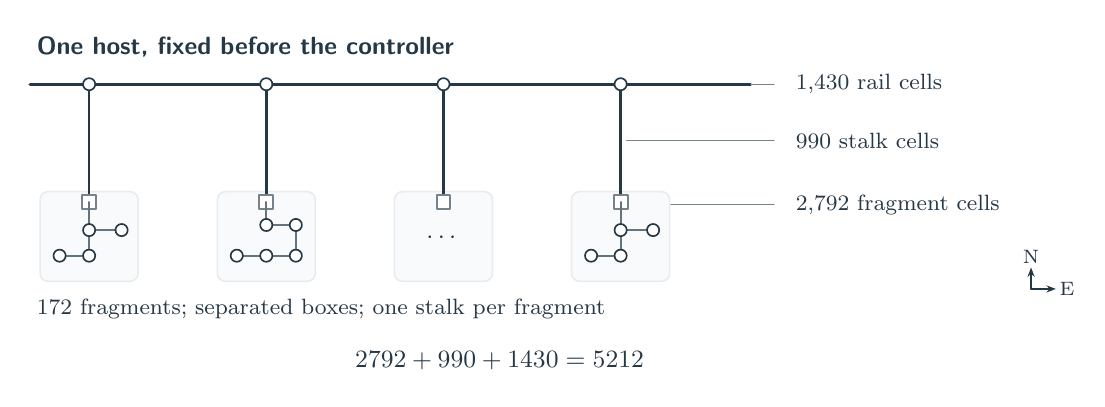
\begin{tikzpicture}[maze,x=7.5mm,y=6.5mm]
 \draw[rvInk,line width=1.15pt] (.3,3.75)--(12.5,3.75);
 \node[paneltitle] at (.25,4.48) {One host, fixed before the controller};
 \foreach \x in {1.3,4.3,7.3,10.3}{
  \draw[lightpanel] (\x-.83,-.1) rectangle (\x+.83,1.65);
  \draw[rvInk,line width=.95pt] (\x,1.45)--(\x,3.75);
  \node[cell] at (\x,3.75) {};
  \node[gate] at (\x,1.45) {};
 }
 % Representative schematic trees inside three fragment boxes.
 \draw[edge] (.8,.4)--(1.3,.4)--(1.3,1.45); \draw[edge] (1.3,.9)--(1.85,.9);
 \draw[edge] (3.8,.4)--(4.3,.4)--(4.8,.4)--(4.8,1)--(4.3,1)--(4.3,1.45);
 \draw[edge] (9.8,.4)--(10.3,.4)--(10.3,1.45); \draw[edge] (10.3,.9)--(10.85,.9);
 \foreach \x/\y in {.8/.4,1.3/.4,1.3/.9,1.85/.9,3.8/.4,4.3/.4,4.8/.4,4.8/1,4.3/1,9.8/.4,10.3/.4,10.3/.9,10.85/.9}{\node[cell] at (\x,\y) {};}
 \node at (7.3,.75) {$\cdots$};
 \draw[rvMid,line width=.4pt] (12.5,3.75)--(12.9,3.75);
 \draw[rvMid,line width=.4pt] (10.4,2.65)--(12.9,2.65);
 \draw[rvMid,line width=.4pt] (11.15,1.4)--(12.9,1.4);
 \node[note] at (13.1,3.75) {$1{,}430$ rail cells};
 \node[note] at (13.1,2.65) {$990$ stalk cells};
 \node[note] at (13.1,1.4) {$2{,}792$ fragment cells};
 \node[note] at (.25,-.65) {$172$ fragments; separated boxes; one stalk per fragment};
 \node[font=\small\bfseries] at (8.25,-1.65) {$2792+990+1430=5212$};
 \mazeCompass{17.25}{-.25}
\end{tikzpicture}

\caption{Universal-host assembly, shown schematically. Each separated fragment joins the
rail through one stalk; the three displayed cell counts are disjoint contributions
to the exact construction.}
\label{fig:global-rail}
\end{figure}

The exact audited realization contains $2{,}792$ cells in the disjoint ported
fragments, $990$ stalk cells strictly between the fragment ports and the rail, and
$1{,}430$ rail cells.  Hence
\begin{equation}
\label{eq:universal-maze-count}
  |U|=2792+990+1430=5212.
\end{equation}
Its induced graph has $5{,}211$ edges and maximum degree $3$.

\begin{theorem}[One universal two-state maze]
\label{thm:universal-5212}
There exists a fixed finite connected induced grid tree $U$ with $5{,}212$ cells and
maximum degree three such that for every legal deterministic controller $A$ with at
most two states there are state-$0$ starts $x_A,y_A\in U$, with
$\|x_A-y_A\|_1\ge2$, for which the two copies of $A$ never reach Manhattan distance
at most one.  Equivalently, the quantifier order is
\[
  \boxed{\exists U\;\forall A\;\exists(x_A,y_A).}
\]
\end{theorem}

\begin{proof}
Fix $A$.  The case tree and Theorem~\ref{thm:human-finite-basis} choose a
terminal source trap together with one simultaneous compass normalization.  Its
inverse-transported oriented instance is represented among the fixed ported fragments.
For a path leaf, its proved full-execution unused cut gives the protected embedding;
for G2 use the unvisited gate; for G1 use the clean-$V$/unused-$JB$ dichotomy.  The
local attachment lemmas preserve the complete unsuccessful execution.  The separated
global placement adds no new neighbor to any cell visited by that execution, so it is
preserved once more in the same fixed maze $U$.  Only the choice of fragment and its
recorded start pair depends on $A$.
\end{proof}

The obstruction basis and portability lemmas prove existence constructively.
The exact $5{,}212$-cell placement is separately validated from all $172$ fragment
records, their starts and embeddings, and the final induced graph; coordinate
verification does not replace the assembly proof.

\subsection{The universal-maze parameter}
\label{subsec:universal-maze-parameter}

Theorem~\ref{thm:universal-5212} suggests a parameter different from the
controller-dependent quantity $F(2)$.  Let
\[
\begin{split}
 u_2=\min\bigl\{|U|:\;& U\text{ is a finite connected induced grid maze and }\\
 &\forall A,\ |Q_A|\le2,\ \exists x_A,y_A\in U\text{ trapping }A\bigr\},
\end{split}
\]
where the starts are state-$0$ and initially noncontacting.  Theorem~\ref{thm:universal-5212}
shows that this minimum is finite and gives $u_2\le5212$.

\begin{corollary}[Every exact size above the construction]
\label{cor:universal-exact-size}
For every integer $n\ge5212$ there exists a universal induced grid tree of maximum
degree three with exactly $n$ cells.
\end{corollary}

\begin{proof}
Extend the exposed right end of the top rail by an induced horizontal ray of exactly
$n-5212$ new cells.  In the explicit placement the first new cell is at Manhattan
distance $8$ from the union of all copied original gadget-cell images, a superset of
every preserved witness trajectory; distances only increase farther along the ray.
Thus no mask queried by any preserved witness changes.  The first new cell has only the
old rail endpoint as an old neighbor, so the extension is a path attached at one
vertex.  Connectedness, acyclicity, inducedness, and maximum degree three are
preserved.
\end{proof}

The opposite direction is currently computational.

\begin{proposition}[Computer-assisted lower bound]
\label{prop:u2-lower-eight}
The universal-maze parameter satisfies
\[
  u_2\ge8.
\]
Consequently
\[
  \boxed{8\le u_2\le5212.}
\]
\end{proposition}

\paragraph{Verification basis.}
The lower bound is a quantifier-reversal statement.  It does not follow from the fact
that every individual two-state controller has some trap on at most seven cells.
Instead, an exhaustive checker enumerates every connected fixed induced grid cell set
through size seven and tests the eight compass conjugates of the extremal controller
$A^\star$.  The controller $A^\star$ has no trap below seven cells.  Among all
seven-cell geometries, a single fixed geometry traps at most four of the eight
conjugates, even when its start pair may be chosen separately for each conjugate.
Thus no maze with at most seven cells is universal for this eight-controller subset.
This proposition is computer-assisted; no deductive classification of all seven-cell
universal candidates is claimed.

It is also useful to isolate the tree-restricted version
\[
 u_{2,\mathrm{tree3}}
 =\min\bigl\{|U|:\ U\text{ is universal and is an induced grid tree with }
 \Delta(U)\le3\bigr\}.
\]
The construction proves
\[
  8\le u_2\le u_{2,\mathrm{tree3}}\le5212,
\]
while neither minimum is known.

The displayed universal-host quantifiers concern distance-one failure, not the
classical exploration-trap parameter of Section~\ref{sec:related}.
\paragraph{Sharpness data for $A^\star$.}
Minimal seven-cell traps of the extremal controller are not all trees; the exhaustive
supplementary data also contain cyclic mechanisms.  No detailed classification of
those traps is needed for Theorem~\ref{thm:universal-5212}.

\section{Related work}
\label{sec:related}

The relevant comparisons concern three different tasks: visiting every vertex or
edge, meeting at one vertex, and the distance-one contact required here. They also
involve different ways of supplying direction information and different orders of
quantification over controllers, graphs, labellings and starts. We organize the
comparison around these distinctions, rather than treating all finite-state walkers
as one model.

\paragraph{Labyrinth automata, quantitative traps, and universal hosts.}
Budach's work on labyrinth exploration~\cite{Budach1978} and the universal-trap
paper of Antelmann, Budach and Rollik~\cite{AntelmannBudachRollik1979} are central
historical predecessors. For their historical theorem statements we rely on the
account of Kilibarda, Kudryavtsev and U\v{s}\'{c}umli\'{c}~\cite{KilibardaKudryavtsevUscumlic2003},
not on uninspected originals. Hemmerling's monograph explicitly treats traps with a
specified starting position and estimates their size in terms of internal
states~\cite[pp.~133--134]{Hemmerling1989}. Thus neither state-dependent trap size
nor a controller-dependent adversary is a new organizing principle.

The observation interface can also be quite close. Hoffmann's inspected opening
pages define plane mazes as full sublabyrinths of the square lattice, with free
compass directions observed locally, and state a one-pebble exploration
impossibility~\cite[pp.~433--434]{Hoffmann1981}. His finite-automaton definition
uses a legal move at every step. Induced geometry and compulsory motion therefore
do not, by themselves, separate our problem from that literature. What must still
be transferred is the objective: an unvisited vertex is not a certificate that two
moving copies always remain nonadjacent.

A quantitative predecessor makes this limitation especially concrete.
The survey~\cite[Theorem~4, p.~25]{KilibardaKudryavtsevUscumlic2003} attributes to
Antelmann a proper planar exploration trap of size at most
$C\exp\sqrt{2s\log_2(2s)}$ for an initialized $s$-state automaton. The cited statement
does not specify a numerical $C$. Antelmann's original article and dissertation
remain uninspected; neither an exact low-state constant nor a rendezvous conclusion
is inferred from this asymptotic bound.

Universal traps require an equally explicit qualification. Kilibarda proves
universal exploration traps for finite families of automata~\cite[Theorems~1.2--1.3]{Kilibarda1990}.
His later reduction paper gives a finite mosaic trap for each finite collective of independent automata and,
in a separate theorem, one \emph{infinite} mosaic trap for all such
collectives~\cite[Theorems~3.5 and~3.8]{KilibardaReduction2021}. Consequently our
finite obstruction menu and fixed host are not presented as the invention of
universal trapping. The specific assembly preserves the complete masks queried by
two executions, produces an explicitly bounded finite induced subcubic grid tree,
and permits only the bad starts to depend on the controller. Its failure predicate
is perpetual nonadjacency. The earlier exploration theorems are genuine quantifier
predecessors, but none of the cited statements supplies that entire conclusion.

\paragraph{Finite-state exploration, exact small memory, and periodic traversal.}
Graph exploration supplies both asymptotic and exact-state comparisons. The work
of Fraigniaud, Ilcinkas, Peer, Pelc and Peleg~\cite{FraigniaudEtAl2005} studies
port-based automata; a modern account of the space-complexity setting is given by
Disser and Klimm~\cite{DisserKlimm2022}. The latter also makes explicit why vertices
with the same observed incident colours are indistinguishable. This is a useful
neighbor of our repeated-mask requirement, although exploration is a one-agent
objective and its label conventions are not an absolute compass.

The closest numerical trap bound is particularly important to acknowledge.
Ilcinkas~\cite[Theorem~2.1, p.~52]{Ilcinkas2006} constructs, for every $K$-state
port-based Moore automaton and $d\ge3$, a simple-graph exploration trap with at most
$K+d+2$ vertices and maximum degree $d$. Substituting $K=2,d=3$ gives seven.
The construction leaves a \emph{vertex} unvisited, so an edge-versus-vertex slogan
would not distinguish it from our theorem. Instead, a transfer must preserve the
controller interface and induced-grid geometry and must create a nonadjacent pair
of executions. No such state-preserving transfer is established here.

Exact one- and two-state classifications are also already available, rather than
being a new kind of question. Fraigniaud, Ilcinkas and
Pelc~\cite{FraigniaudIlcinkasPelc2008} classify regular graphs explorable by
port-Mealy automata: the one-state class consists of the one-vertex graph, $K_2$ and
cycles, while the two-state class consists of cliques and cycles. An automaton for
a graph must work for every port assignment and initial position. These are strong
predecessors for the small-memory viewpoint, but not determinations of our
max--min trap parameters for a fixed compass-mask interface.

For the structural results, Diks, Fraigniaud, Kranakis and
Pelc~\cite{DiksEtAl2004} already use a degree-based state lower bound and the
cyclic next-port rule for perpetual tree exploration. Kilibarda's
Proposition~1.1~\cite{Kilibarda1990} states that every rotation system of a tree
induces one contour; the same paper gives exact small-state exploration thresholds
in a richer local-vision model. Thus the contour mechanism in
Section~\ref{sec:paths} is classical. Our four-state table stores the incoming
\emph{compass} port internally, because it is not supplied as an observation;
the radius-one rendezvous conclusion additionally uses path phase contact.
This is not a per-vertex rotor-memory model: the fixed tree has no writable local
state.

Periodic exploration is another close, but different, extremal problem.
Ilcinkas~\cite{Ilcinkas2008Ports} gives a three-state explorer with period at most
$4n-2$ after a suitable port assignment. That problem minimizes a guaranteed
exploration period while permitting the designer to choose local orientations;
its configurations include an incoming port. Our sharp-period theorem instead
maximizes the least tagged period over allowed compass paths and controllers,
under an internal-state budget. Neither the periodic-exploration bound nor the
standard contour alone gives the weighted capacity and sharp all-state formula
proved in Section~\ref{sec:support-structure}.

\paragraph{Meeting identical agents: resources and port quantifiers.}
Pelc's survey provides the broader deterministic network-rendezvous
context~\cite{Pelc2012Survey}. A particularly relevant compass-labyrinth result is
Kilibarda's type-meeting theorem~\cite[Theorem~10]{Kilibarda2021}. Its strong version
uses two copies of one collective and same-vertex contact; the minimal universal
types for finite mosaic labyrinths are $(1,2)$ and $(2,0)$. A type counts active
automata and pebbles, not internal states. In particular, copying a collective of
type $(2,0)$ is not a theorem about two single agents. The negative side concerns
same-vertex meeting and does not supply a distance-one trap or the exact values
four, seven or eight in our model.

Bounded-memory rendezvous in port-labelled graphs is more developed than a
comparison based only on a few constants would suggest. Czyzowicz, Kosowski and
Pelc~\cite{CzyzowiczEtAl2012} establish log-space rendezvous bounds in arbitrary
graphs. For trees, the distinction between the following two domains is essential.
Fraigniaud and Pelc~\cite[Definitions~1.1--1.2 and Section~1.2]{FraigniaudPelc2011}
require success for every port labelling and restrict admissible initial pairs by
perfect symmetrizability. Their simultaneous-start result does not cover every pair
that happens to be nonsymmetric under one fixed labelling. Czyzowicz, Kosowski and
Pelc~\cite{CzyzowiczEtAl2014} prove a logarithmic memory lower bound even for
simultaneous starts on lines in that latter, broader domain. The inspected author
versions explicitly expose the correction to the earlier conference formulation.
These are not conflicting bounds once the domains are kept distinct.

Those models supply arrival-port information, permit waiting, and require
same-node meeting. Our compass, compulsory motion, identical initial states and
integer-time distance-one event must therefore all be retained when comparing the
path threshold or the still-open three-state case. In particular, a lower bound on
same-node rendezvous is not automatically a lower bound on distance-one contact,
even if it already applies to simultaneous starts.

\paragraph{Recent nearby models.}
The 2026 preprint of Das and Pelc~\cite{DasPelc2026} is a close current finite-state
comparison: it asks for a universal deterministic automaton on all feasible
rendezvous instances of port-labelled graphs. Its negative result with finitely
many stationary pebbles already has simultaneous-start line witnesses.
Thus start delay alone cannot explain the separation from our positive path
result. The same-node predicate, port observations and feasibility quantifiers
remain decisive; the preprint does not settle our three-state question.

Recent grid and neighborhood work illustrates two other boundaries.
Gao and Pelc~\cite{GaoPelc2025} study identical agents with a coherent compass on
the infinite grid, but allow waiting and permanent footprints, and require a common
node. Eguchi, Kitamura and Izumi's \emph{neighborhood rendezvous}~\cite{EguchiEtAl2022}
assumes initially adjacent agents and still seeks same-node meeting; it does not
mean success at distance one. Its randomized, labelled-graph setting is also not a
fixed small-state anonymous controller. These papers clarify model choices rather
than provide numerical predecessors to our trap thresholds.

\paragraph{Graph-walking realization and deterministic synthesis.}
Local descriptions of finite-state computations have strong precedents.
Martynova~\cite{Martynova2022} encodes graph-walking computations by attaching
incoming and outgoing state sets to directions and imposing node consistency.
Theorem~5 of the inspected author version transforms a \emph{given} automaton
into a signature describing accepted graphs. Here a graph and a cyclic scenario
are prescribed, while the common transition table is unknown. This reverses the
synthesis direction; it does not make the use of local state annotations itself
new.

Similarly, Ulyantsev, Buzhinsky and Shalyto~\cite{UlyantsevBuzhinskyShalyto2016}
identify deterministic machines from scenarios using state assignments and
transition consistency. Our occurrence-colouring formulation belongs naturally to
this exact-synthesis neighborhood. The content specific to
Theorem~\ref{thm:three-state-realization} is a normal form for a restricted recurrent
scenario: arbitrary row outputs are eliminated in favor of a finite common
mask/difference profile and one bit per internal vertex. It is not a general theorem
that scenario synthesis is new or that local annotations guarantee global
realizability without further constraints.

\paragraph{Algebraic consistency and the scope of the contribution.}
Signed-graph balance and switching are classical; see
Zaslavsky~\cite[Section~2, Proposition~2.1]{Zaslavsky1982}. Gain graphs generalize
edge signs to group elements, with identity product around balanced
cycles~\cite{Zaslavsky1989}. This is the correct context for our signed-graph
special cases, but not for the entire realization criterion. A profile system may
have rows involving more than two bits; it balances all linear dependencies of one
matrix. Successor differences may be zero, and the existential choice of one common
profile can produce non-affine phase projections. Replacing the full criterion by
one signed graph or by permutation-only transport would change the theorem.

Nor is polynomial recognition at a fixed state budget and alphabet asserted as a
new complexity result: the set of complete controller tables is already finite
independently of path length. The contribution claimed here is the proved
combination of the exact model-specific trap thresholds, weighted recurrent-support
bounds with sharp attainment, the special affine realization normal form, and
observation-preserving obstruction assembly. The inspected predecessors do not
supply this combination under the same hypotheses. That comparison is not an
absolute priority claim; the access limitations on historical originals remain
explicit.

\section{Open problems}\label{sec:open-problems}

The remaining questions concern the interface between recurrence, accessibility and
uniformity, rather than a missing numerical adjustment to the proved thresholds.
The three-state path question is
\[
 F_{\mathcal P,1}(3)\ ?
\]
Equivalently, does one three-state controller solve every finite induced path, or
does the eventual path state complexity become four? The realization theorem decides
whether a prescribed contour-plus-matching cycle can exist. It does not decide whether
one fixed controller has the required state-zero-accessible basin structure on every
path. The unrestricted-grid quantity $F_{\mathcal G,1}(3)$ is also open; branching
invalidates the path phase-contact argument even on a unique recurrent cycle.

The exact minimum universal-host size $u_2$ and its subcubic-tree analogue
$u_{2,\mathrm{tree3}}$ are unknown. The current range
$8\le u_2\le u_{2,\mathrm{tree3}}\le5212$ combines a computer-assisted lower bound
with an explicit construction. It neither proves that $5212$ is optimal nor transfers
the individual-controller threshold seven to the one-host quantifier order.
Let $b_2$ be the minimum cardinality of an arbitrary finite complete test family.
The certified selection gives $b_2\le44$; the packing witness proves optimality only
inside the fixed $144$ candidates, and the global minimum remains open.

Beyond one state there is no exact higher-memory radius law here. The sharp period
formula determines the maximum recurrent period over path geometries, not the
realizability of every weighted walk by a common table. A full higher-state realization
theory, including arbitrary four-state path normal forms, also remains open. These
questions should preserve the distinctions between least tagged period and spatial
period, between actual masks and support masks, and between a constructed cycle and
its accessibility. None is resolved by extending a finite scan horizon.

\FloatBarrier
\appendix
\section{Local obstructions for the upper bound}\label{u:appendix}

This appendix supplies the mixed-axis and corner-bit arguments used
in Section~\ref{u:section}. Coordinates, masks, and next-state bits
have the notation of that section. Every pair of starts below is
in state zero. All displayed geometries are induced paths: for an
$L$ or $U$ this follows from its defining coordinates, and for each
listed endpoint order no nonconsecutive pair is at unit distance.

\subsection{Excluding one reset axis}\label{u:appendix-mixed}

\begin{lemma}\label{u:mixed0}
A path survivor cannot have vertical straight map $C_0$ and
horizontal straight map $I$ in the frame of Lemma~\ref{u:axis}.
\end{lemma}

\begin{proof}
Here
$\delta(0,\mathrm{NS})=(\Sdir,0)$,
$\delta(1,\mathrm{NS})=(\N,0)$, and $n_0=e_0=1$.
We force three corner rows and then contradict survival. Every
unlisted corner or endpoint bit remains arbitrary.

\emph{The ES state-zero row must be $(\Sdir,0)$.}
If it chooses east, use $L(\Sdir,\E;3,2)$ with starts $S_2,C$.
The southern agent stays in the reset pocket $S_1,S_2,S_3$.
The corner-started agent stays in $C,E_1,E_2$: every return to $C$
from the horizontal straight cell has state zero, and that corner
row sends it east. The disjoint regions and even-colored starts
give a trap.
If instead the row is $(\Sdir,1)$, use $L(\Sdir,\E;4,1)$
with starts $S_4,C$. The southern agent stays in $S_2,S_3,S_4$,
with $S_2$ visited only in state zero: from $S_3$ either state
reaches $S_2$ or $S_4$ in state zero, and the endpoint returns
to $S_3$ in either state. The other agent has exact cycle
$C_0\to(S_1)_1\to C_0$. The regions are disjoint and the starts
are even. Only $(\Sdir,0)$ remains.

\emph{The SW state-zero row must point west.}
Use the upward U with endpoint order
\[
(0,0),(0,1),(0,2),(1,2),(2,2),(2,1),(2,0)
\]
and starts $(0,1),(2,1)$. Every arrival at either upper corner
from its straight vertical arm has state zero. The ES corner
returns south by the row just forced. If the SW state-zero row
also chose south, both vertical columns would be closed and
two units apart. Thus SW in state zero chooses west.

\emph{The SW state-one row must be $(\Sdir,0)$.}
If it chooses west, use $L(\Sdir,\W;3,2)$ with starts $S_3,W_1$.
The pocket's closed tagged set contains $(S_3)_0$.
The other agent begins
\[
(W_1)_0\to(W_2)_0\to(W_1)_1\to C_1,
\]
using $e_0=1$. Every later arrival at $C$ from the west arm also
has state one, so that arm, including $C$, is closed. The regions
are disjoint and both starts are odd.
If the row is $(\Sdir,1)$, use $L(\Sdir,\W;4,2)$ with starts
$S_4,W_2$. The southern agent remains in $S_2,S_3,S_4$ as above.
The other begins $(W_2)_0\to(W_1)_1\to C_1$ and then
\[
C_1\to(S_1)_1\to C_0.
\]
The already forced west-pointing state-zero row returns it to the
west arm; every return from that arm reaches $C_1$.
Thus its whole trajectory lies in $W_2,W_1,C,S_1$, with $S_1$
visited only in state one. These regions are disjoint and the
starts are even. This excludes the second alternative and forces
$(\Sdir,0)$.

\emph{The forced rows give a trap.}
Use
\[
(0,0),(0,1),(0,2),(1,2),(2,2),(2,1)
\]
with starts $(0,1),(2,1)$. The left three-cell column is closed
by the vertical reset and the ES state-zero row. The right agent
has exact cycle
\[
(2,1)_0\to(2,2)_1\to(2,1)_0
\]
by $n_0=1$ and the SW state-one row. Their horizontal coordinates
remain zero and two, respectively. This contradicts path survival.
\end{proof}

\begin{lemma}\label{u:mixed1}
A path survivor cannot have vertical straight map $C_1$ and
horizontal straight map $I$ in the frame of Lemma~\ref{u:axis}.
\end{lemma}

\begin{proof}
Now
$\delta(0,\mathrm{NS})=(\Sdir,1)$,
$\delta(1,\mathrm{NS})=(\N,1)$, and $e_0=1$.
Reset pockets point north. We keep the initial state zero throughout;
in particular, the free bit $s_1$ is treated in both of its cases.

\emph{The NW state-one row must be $(\N,1)$.}
If it chooses west, use $L(\N,\W;3,2)$ with starts $N_2,W_2$.
The north pocket is closed, while the other agent starts
$(W_2)_0\to(W_1)_1\to C_1$. Every later arrival from the west
arm has state one, so its west-pointing corner row closes
$W_2,W_1,C$. The regions are disjoint and the starts are even.
If the row is $(\N,0)$, use $L(\N,\W;4,1)$ with starts $N_3,W_1$.
The first agent stays in $N_2,N_3,N_4$: the closed pocket tagged
set is $\{(N_2)_1,(N_3)_0,(N_3)_1,(N_4)_1\}$.
The second has prefix $(W_1)_0\to C_1$ followed by
$C_1\to(N_1)_0\to C_1$.
The disjoint regions and odd starts again give a trap.
This leaves only $(\N,1)$.

\emph{The NE state-one row must point east.}
Use the downward U, namely $U(\N,\E)$, with starts
$(0,1),(2,1)$. Both arrivals at the lower corners from their
vertical arms have state one. The right NW corner returns north.
If the left NE state-one row also chose north, both columns would
be closed and two units apart. It must therefore choose east.

\emph{The NE state-zero row must be $(\N,1)$.}
If it also chooses east, use $L(\N,\E;3,2)$ with starts $N_2,E_2$.
The north pocket is closed, and both corner states point east,
closing $C,E_1,E_2$. The regions are disjoint and the starts even.
If the row is $(\N,0)$, use $L(\N,\E;4,2)$ with starts $N_4,E_2$.
The first endpoint move reaches $N_3$ in either state. From there,
state zero reaches $(N_2)_1$ and state one reaches $(N_4)_1$;
thereafter $N_2,N_3,N_4$ remains closed, with $N_2$ only in state
one. The second agent stays in $C,E_1,E_2,N_1$. Its only northern
excursion is $C_0\to(N_1)_0\to C_1$, and the state-one corner
row sends it east. The regions are disjoint and the original
starts even. Hence the remaining row is $(\N,1)$.

\emph{Both values of $s_1$ now give a trap.}
For $s_1=0$, use
\[
(0,1),(0,0),(1,0),(2,0),(2,1),(2,2)
\]
with starts $(0,0),(2,2)$. The left agent has exact cycle
$(0,0)_0\to(0,1)_1\to(0,0)_0$.
The right column is closed because every corner arrival from
its straight cell has state one and the NW row returns north.
The columns are two units apart from time zero.
For $s_1=1$, use $U(\N,\E)$ with starts $(0,0),(2,1)$.
The complete entry prefixes are
\[
\begin{array}{l}
(0,0)_0\to(0,1)_1\to(0,2)_1,\\
(2,1)_0\to(2,0)_1\to(2,1)_1\to(2,2)_1.
\end{array}
\]
Each is then followed by its upper edge in state one. Again the
agents remain in their separate columns throughout. These two
cases exhaust the endpoint bit and contradict path survival.
\end{proof}

\subsection{The four corner output bits}\label{u:appendix-bits}

\begin{lemma}\label{u:bit-laws}
Assume identity straight maps, $n_0=e_0=1$, and the direction
conclusions
\[
\operatorname{dir}\delta(0,\mathrm{NE})=\E,\quad
\operatorname{dir}\delta(0,\mathrm{ES})=\Sdir,\quad
\operatorname{dir}\delta(1,\mathrm{ES})=\E,\quad
\operatorname{dir}\delta(1,\mathrm{SW})=\Sdir.
\]
If the controller survives all induced paths through seven cells,
their output states are, respectively, $1,0,1,0$.
\end{lemma}

\begin{proof}
Each of the following six-cell paths excludes one wrong bit,
independently of the other three output-bit conclusions.

\emph{ES in state zero cannot output one.}
Suppose $\delta(0,\mathrm{ES})=(\Sdir,1)$ and use
\[
(1,2),(0,2),(0,1),(0,0),(1,0),(2,0)
\]
with starts $C=(0,0)$ and $U=(0,2)$.
Write $M=(0,1)$, $H=(1,0)$, $E=(2,0)$, and $P=(1,2)$.
The first agent stays in $C,H,E$: every return from $H$ reaches
$C$ in state zero, whose NE row points east.
The second has closed tagged set
\[
\{U_0,U_1,M_1,P_0,P_1\}.
\]
Indeed $U_0\to M_1\to U_1$, the ES state-one row points to $P$,
and endpoint $P$ returns to $U$ in either state. The two spatial
regions are disjoint and the starts even, proving failure.

\emph{ES in state one cannot output zero.}
Suppose $\delta(1,\mathrm{ES})=(\E,0)$ and use
\[
(0,1),(0,2),(1,2),(2,2),(2,1),(2,0)
\]
with starts $P=(0,1)$ and $I=(2,1)$.
Put $C=(0,2)$, $H=(1,2)$, $D=(2,2)$, $B=(2,0)$.
The left prefix is
$P_0\to C_1\to H_0\to C_0$.
At $C_0$ the ES row points south to $P$, whose endpoint return
may reach either state of $C$. Thus $P,C,H$ is closed, with $H$
only in state zero. The right arm $B,I,D$ is closed: every
arrival at $D$ from $I$ has state one and its SW row points south.
The regions are disjoint and both starts odd.

\emph{NE in state zero cannot output zero.}
Suppose $\delta(0,\mathrm{NE})=(\E,0)$ and use
\[
(0,3),(0,2),(1,2),(2,2),(2,1),(2,0)
\]
with starts $(1,2),(2,1)$.
The first agent has exact cycle $(1,2)_0\leftrightarrow(0,2)_0$.
The second stays in the right three-cell column by the
state-one SW direction and the corner-arrival rule.
The spatial regions are disjoint and both starts odd.

\emph{SW in state one cannot output one.}
Suppose $\delta(1,\mathrm{SW})=(\Sdir,1)$ and use
\[
(0,2),(1,2),(1,1),(1,0),(2,0),(3,0)
\]
with starts $(0,2),(2,0)$.
The upper agent's complete prefix and cycle are
\[
(0,2)_0\to(1,2)_1\to(1,1)_1\to(1,2)_1\to\cdots,
\]
using $e_0=1$. The lower agent stays in the horizontal arm
$(1,0),(2,0),(3,0)$: every arrival at its NE corner $(1,0)$
has state zero and is sent east. The regions are disjoint and
both original starts even. This excludes the last wrong bit.
\end{proof}

\section{Complete short-twig maps}\label{c:twig-appendix}

This appendix completes the local calculation used in
Lemma~\ref{c:twig}. Attach a path \(p-u-v\), where \(u\) has exactly
the two neighbours \(p,v\) and \(v\) is a leaf. Write \(de\) for the
directions \(p\to u\) and \(u\to v\). The condition \(e\ne-d\)
ensures that the three vertices are distinct and leaves exactly twelve
words. We stop upon returning to \(p\), so its other neighbours and
outgoing rule play no role in this table.

\begin{table}[htbp]
\centering\small
\setlength{\tabcolsep}{4pt}
\begin{tabular}{lllllll}
\toprule
\(de\) & Masks at \(u,v\) & \(u_0\to\) & \(u_1\to\)
& \(v_0\to\) & \(v_1\to\) & Return or internal cycle \\
\midrule
\(\N\N\)&\(\N\Sdir,\Sdir\)&\(p_1\)&\(p_1\)&\(u_1\)&\(u_1\)&All return as 1\\
\(\N\E\)&\(\E\Sdir,\W\)&\(p_1\)&\(v_1\)&\(u_1\)&\(u_0\)&All return as 1\\
\(\N\W\)&\(\Sdir\W,\E\)&\(v_0\)&\(p_1\)&\(u_1\)&\(u_1\)&All return as 1\\
\(\E\N\)&\(\N\W,\Sdir\)&\(v_1\)&\(p_0\)&\(u_1\)&\(u_1\)&All return as 0\\
\(\E\E\)&\(\E\W,\W\)&\(p_0\)&\(v_1\)&\(u_1\)&\(u_0\)&All return as 0\\
\(\E\Sdir\)&\(\Sdir\W,\N\)&\(p_0\)&\(v_1\)&\(u_0\)&\(u_1\)&\(u_0,v_0\) return; \((u_1,v_1)\)\\
\(\Sdir\E\)&\(\N\E,\W\)&\(p_0\)&\(v_1\)&\(u_1\)&\(u_0\)&All return as 0\\
\(\Sdir\Sdir\)&\(\N\Sdir,\N\)&\(v_1\)&\(v_1\)&\(u_0\)&\(u_1\)&All reach \((u_1,v_1)\)\\
\(\Sdir\W\)&\(\N\W,\E\)&\(p_1\)&\(v_0\)&\(u_1\)&\(u_1\)&\(u_0\) returns; \((u_1,v_0)\)\\
\(\W\N\)&\(\N\E,\Sdir\)&\(v_0\)&\(p_1\)&\(u_1\)&\(u_1\)&All return as 1\\
\(\W\Sdir\)&\(\E\Sdir,\N\)&\(v_1\)&\(p_1\)&\(u_0\)&\(u_1\)&All return as 1\\
\(\W\W\)&\(\E\W,\E\)&\(v_0\)&\(p_1\)&\(u_1\)&\(u_1\)&All return as 1\\
\bottomrule
\end{tabular}
\caption{Complete stopped maps for two-cell twigs. Every arrow is a
substitution in Table~\ref{tab:astar}. Parentheses in the final column
denote the unique internal tagged cycle in the specified row.}
\label{c:twig-table}
\end{table}

For the \(\N\E\) row, the longest return is
\(v_0\to u_1\to v_1\to u_0\to p_1\); all other starting tags give
suffixes of this route. The \(\E\E\) and \(\Sdir\E\) rows have the
same four-step form, returning to \(p_0\). In each of the remaining
nonabsorbing rows, the printed arrows give a return in at most four steps.
For \(\E\Sdir\), the tags \(u_1,v_1\) form the displayed cycle and
\(v_0\to u_0\to p_0\). For \(\Sdir\Sdir\),
\(v_0\to u_0\to v_1\) joins \((u_1,v_1)\). For \(\Sdir\W\),
\(v_1\to u_1\) joins \((u_1,v_0)\), while \(u_0\to p_1\).
These routes verify every transient and every internal recurrent component.

For a one-cell twig in direction \(d\), the leaf has mask \(\{-d\}\).
The endpoint rows therefore return state one for
\(d\in\{\N,\W\}\), preserve the arriving state for \(d=\Sdir\),
and complement it for \(d=\E\).

\subsection*{The permitted square ports}

Use the absolute square coordinates
\(a=(0,0),b=(1,0),c=(1,1),d=(0,1)\). In family \(\mathsf Q\)
there are at most two exterior cells and no second square. For a two-cell
twig at \(c\N\), a west continuation would meet the northwest corner,
so the only words are \(\N\N,\N\E\). The same grid-edge check gives
\(\E\E,\E\N\) at \(c\E\),
\(\N\N,\N\W\) at \(d\N\), and
\(\W\W,\W\N\) at \(d\W\).
All these rows return every tag. This excludes an attractor in a dormant
twig even for a trajectory that starts there.

The four active ports have the complete behaviour in
Table~\ref{c:active-ports}. The entry tag is obtained from the square
corner table. The one-cell column records the return of that entry tag;
an arbitrary tag on a one-cell twig also returns immediately, possibly in
the other state. The all-tag assertions in the two-cell column include
all four tags, not merely the tag entering from the core.

\begin{table}[htbp]
\centering\small
\begin{tabularx}{\textwidth}{llllX}
\toprule
Port & Entry tag & One cell & Two-cell word & Complete effect \\
\midrule
\(a\Sdir\)&\(u_1\)&Return \(a_1\)&\(\Sdir\Sdir\) or \(\Sdir\W\)&
The entering tag reaches the internal edge cycle. In the second word only
\(u_0\) returns to \(a_1\).\\
\addlinespace
\(a\W\)&\(u_0\)&Return \(a_1\)&\(\W\W\) or \(\W\Sdir\)&
Every tag returns to \(a_1\).\\
\addlinespace
\(b\E\)&\(u_1\)&Return \(b_0\)&\(\E\E\) or \(\E\Sdir\)&
The first word returns every tag to \(b_0\). The second captures the
entry tag; \(u_0,v_0\) return to \(b_0\).\\
\addlinespace
\(b\Sdir\)&\(u_0\)&Return \(b_0\)&\(\Sdir\E\) or \(\Sdir\Sdir\)&
The first word returns every tag to \(b_0\). The second captures every
tag on its outer state-one edge.\\
\bottomrule
\end{tabularx}
\caption{Active square-port returns and absorbers. The one-cell return
uses the listed entry tag. The two-cell options exclude continuations
that make a second square.}
\label{c:active-ports}
\end{table}

In the \(a\Sdir\) case with word \(\Sdir\W\), the returnable tag
does not become trapped within the stopped twig map: the square sends it
\(u_0\to a_1\to b_1\to a_0\to u_1\), after which it enters the
absorber. Likewise the returnable tags of the \(\E\Sdir\) twig at
\(b\E\) return to \(b_0\), travel through the square back to
\(b_1\), and are then sent to \(u_1\). These uses of the square core
are part of the proof of Lemma~\ref{c:square}, rather than extra assertions
about an isolated twig.

\section{Affine realization: gauges, elimination and witnesses}
\label{app:realization-bookkeeping}

\subsection{Coordinate choices and unused rows}
The nonzero vectors of $H=\Ftwo^2$ are the three states. Every permutation of them
extends uniquely to an element of $\operatorname{GL}(2,2)\cong S_3$. Applying this
map simultaneously to all state constants, successor differences and occurrence
expressions gives an isomorphic profile system. Swapping the two local paired
roles replaces $z_v$ by $z_v+1$; changing an anchor replaces comparisons by their
sums. Thus the construction does not depend on these presentational choices.
An independent permutation at one mask, without transforming the successor
links to other masks, is not a symmetry. Nor can different occurrences of one
absolute mask be independently rotated by grid symmetries.

At a load-two vertex the unused state is $b(a_M)+a_M(z_v+1)$. It is unused at that
vertex, not necessarily at the other vertices of mask $M$. When both paired input
states occur somewhere at $M$, $\kappa_M$ is their uniquely determined successor
difference. When only one occurs, it is an auxiliary description of the observed
transitions; it does not prescribe an unobserved output. In particular, the
unobserved row must not be assigned an affine extrapolation that equals the zero
vector. The arbitrary legal completion in the sufficiency proof avoids this
error. Endpoint comparisons cannot be dropped even when both endpoints have
load one: identical endpoint masks and states refer to the same controller row.

\subsection{Exact completion by elimination}
\label{app:linear-completion}
Fix one profile and partition its variables into retained variables $x$ and
variables $y$ to be completed. Write the system as
\[
 A_xx+A_yy=b.
\]
For a fixed $x$ there exists a completion precisely when
\[
 \lambda^T A_y=0\quad\Longrightarrow\quad
 \lambda^T A_xx=\lambda^T b.
\]
Indeed, this is exactly the condition that $b-A_xx$ belong to the column space
of $A_y$, by Gaussian elimination. This is the correct completion statement for
load-two roles: additional constraints on retained roles can remain after
elimination. Before fixing a profile the set of completions is a union of these
affine sets and need not itself be affine. An automatic completion assertion
based only on saturated correspondences is therefore not used.

\subsection{Signed graphs and incidence pseudoforests}
\label{app:forest-cases}
In a fixed profile, first combine repeated terms in each scalar equation and
retain constant equations. If every remaining equation has at most two variables,
form a signed multigraph with a reference vertex $*$ of value zero. Represent
$z_u=b$ by an edge $u*$ of gain $b$, and $z_u+z_v=b$ by an edge $uv$ of gain $b$.
Parallel edges are retained. A constant $0=1$ rejects the system.

\begin{proposition}[Graph balance]\label{prop:affine-graph-balance}
After constant equations are checked, such a system is consistent if and only
if the XOR of the gains around every cycle is zero. In particular, a forest is
consistent, and a component with one cycle has exactly its one parity condition.
\end{proposition}
\begin{proof}
A solution telescopes around each cycle. Conversely, choose a root in each
component and propagate values along a spanning tree, fixing the root of the
component containing $*$ to zero. Each non-tree edge is satisfied precisely when
its fundamental cycle has gain zero. This also proves that the solution space
has dimension $c-1$, where $c$ is the number of components including the one
containing $*$.
\end{proof}

The incidence graph of a general scalar system is instead bipartite, with variable
vertices and equation vertices. Its being a forest is \emph{not} by itself a
consistency criterion: the two equations $z=0$ and $z=1$ have an incidence tree.
Use the following exact reductions. Check constant equations; substitute every
unary fixation; discard degree-zero variables as free; and remove a degree-one
variable together with its unique incident equation, saving that equation for
back-substitution. Each reduction preserves existence of a solution. A finite
incidence forest has a leaf, so these reductions decide it completely.
If each incidence component has at most one cycle, the residual nonempty core
has degree two at every vertex and has equations
\[
 z_1+z_2=c_1,\ \ldots,\ z_{k-1}+z_k=c_{k-1},\ z_k+z_1=c_k.
\]
It is consistent precisely when $\sum_i c_i=0$. The constants here are the
\emph{updated} constants after substitution, not necessarily the original ones.
Solving the core and back-substituting reconstructs a solution. All these tests
must use one shared profile across the components.

For the general system an inclusion-minimal inconsistent set of rows is a
minimal binary dependency whose coefficients cancel and whose right-hand sides
sum to one. To see the minimality assertion, a proper coefficient dependency
with right-hand side one would itself contradict minimality; one with right-hand
side zero could be removed, leaving a smaller contradiction. These row circuits,
not necessarily graph cycles, are the general algebraic obstructions. A failed
profile is not a failed specification: every admissible profile must fail.

\subsection{The saturated NAND witness}
\label{app:nand-witnesses}
For the specification of Proposition~\ref{prop:nand8}, the occurrence word is
\[
(0,1,0,1,2,3,2,3,4,5,6,7,6,7,6,5,4,3,2,1).
\]
With ordinary state names $0,1,2$, the following assignments, in this occurrence
order, realize the three allowed pairs of saturated correspondence bits:
\begin{align*}
00:\quad &(0,0,2,1,1,0,2,1,1,1,1,0,2,1,0,2,0,2,0,2),\\
01:\quad &(0,0,2,1,1,0,2,1,1,0,2,1,1,0,0,2,2,2,0,2),\\
10:\quad &(0,0,2,1,1,2,0,1,1,1,1,2,0,1,2,2,0,0,2,2).
\end{align*}
The $x$-bit compares the W-pairs at occurrences $(1,19)$ and $(5,17)$;
the $y$-bit compares the E-pairs at $(4,6)$ and $(10,12)$. Reading the successors
verifies that each repeated $(q,M)$ has the same direction and next state.
States at each spatial vertex are distinct. These explicit assignments establish
the positive cases without an enumeration argument; the main-text four-state
contradiction excludes $11$.

\subsection{The six-vertex staircase}
\label{app:staircase}
Take directions $\E\N\E\N\E$, doubled edge indices $1,3$, and phases $0,1$,
respectively. Its word is
\[
 (0,1,2,1,2,3,4,5,4,3,4,3,2,1).
\]
All four internal vertices are saturated. Put $w=q_{13}=q_{11}$ for the
singleton W-state of mask $\N\W$, and $e=q_4=q_6$ for the singleton E-state
of mask $\E\Sdir$. Let $x$ compare the N-pairs $(q_1,q_3)$ and $(q_5,q_9)$,
and let $y$ compare the S-pairs $(q_2,q_{12})$ and $(q_8,q_{10})$.
The N-rows have successor pairs $(q_2,e)$ and $(e,q_{10})$.
Identity correspondence would force $q_2=e$, contradicting the two different
direction roles at one mask. Hence $x=1$, and the swapped correspondence forces
$q_2=q_{10}$, so $y=1$. The S-rows have successor pairs $(q_3,w)$ and $(q_9,w)$;
$y=1$ would force $q_3=w$, again contradicting distinct roles. Thus $y=0$.
Equivalently these constraints contain
\[
 x=1,\qquad x+y=0,\qquad y=0,
\]
whose sum is $0=1$. This proves impossibility directly. The separate assertion
that no smaller direction-consistent specification is impossible is an exact
finite check, not part of this argument.

\section{Boundary cases and consequences of realization}
\label{app:structural-consequences}

\subsection{One-edge supports with their actual masks}
\begin{lemma}\label{lem:one-edge-realization}
Let a support consist of one edge $uv$, let its directional multiplicity be $k$,
and read the actual ambient masks $M_u,M_v$. An $s$-state simple tagged cycle
exists exactly when $k\le s$ if $M_u\ne M_v$, and exactly when $2k\le s$ if
$M_u=M_v$.
\end{lemma}
\begin{proof}
Each endpoint needs $k$ distinct states. If the masks are equal, the two sets
must be disjoint because their outgoing directions are opposite. These are the
necessary inequalities. If the masks differ, use states $0,\ldots,k-1$ at both
ends and prescribe
\[
 \delta(i,M_u)=(d,i),\qquad
 \delta(i,M_v)=(-d,i+1\bmod k),
\]
where $d$ points from $u$ to $v$. If the masks agree, use disjoint sets with
$\delta(i,M)=(d,k+i)$ and $\delta(k+i,M)=(-d,i+1\bmod k)$.
These rows produce the required cycle and can be completed legally.
\end{proof}
Thus a doubled edge is possible with three states when it is the entire path,
but not when both its endpoints have the same straight ambient mask. The
multiplicity-three exception on an entire one-edge path is outside the
contour-plus-matching input of Theorem~\ref{thm:three-state-realization}.

\subsection{Two-state contours and a strict memory separation}
For a support of at least three vertices, the two-state capacity law forces
every edge multiplicity to be one. This is a necessary normal form, not an
automatic realization theorem. Fix an order of the two ports of every internal
mask $M$, and let $h_M\in\Ftwo$ be the outgoing state for its first port; the
other state is $h_M+1$. Choose endpoint states, giving at most four endpoint
profiles. At internal occurrences group equal $(M,d)$ and equate their successor
states. At endpoints group equal $(M,q)$ and do the same. The resulting equations
in the $h_M$ are scalar XOR equations, including constants.

This criterion is exact. Necessity follows because both states are used at
each internal vertex and its two outgoing directions differ. For sufficiency,
the two assigned states there are distinct, and each repeated controller key
has both its direction and successor fixed consistently by precisely the stated
groups. Complete unused rows legally. Thus one of these at most four systems is
consistent if and only if the ordinary contour is realizable with two states.
There are at most six internal masks, so this particular recognition construction
is linear in the word length for the fixed compass alphabet.

A useful strict separation is the family with directions
\[
 \E^a\N^b\W^c,\qquad a,c\ge2,\quad b\ge3.
\]
Its ordinary contour requires exactly three states. For the two-state
impossibility, let $\alpha$ be the N-state of the $\N\W$ corner and $\beta$ the
S-state of the $\Sdir\W$ corner. The shared E-row of the straight horizontal
mask forces $\alpha=\beta$, by comparing its transitions into the two corners.
The straight vertical N-row compared with the upper corner forces its state to
be $1-\beta$; the vertical S-row compared with the lower corner forces its state
to be $1-\alpha$. These are then equal, contradicting the two directions at a
straight vertical vertex. For sufficiency, the following used rows give one
three-state controller for the whole family; blank rows may be completed legally:
\begin{center}
\begin{tabular}{c@{\qquad}ccc}
\toprule
Mask & State 0 & State 1 & State 2\\
\midrule
$\E\W$ & $(\E,0)$ & $(\W,1)$ & ---\\
$\N\Sdir$ & --- & $(\Sdir,1)$ & $(\N,2)$\\
$\N\W$ & $(\N,2)$ & $(\W,1)$ & ---\\
$\Sdir\W$ & $(\Sdir,1)$ & --- & $(\W,1)$\\
$\E$ & --- & $(\E,0)$ & ---\\
\bottomrule
\end{tabular}
\end{center}
Start at the lower left endpoint in state 1. The horizontal directions use
states 0 and 1, the vertical directions states 2 and 1, and the two corners
use states $(0,1)$ and $(2,0)$. Directly following these rows gives the contour
and distinct tags at each vertex. Minimality of its eight-vertex representative
among all two-state contour failures is only a finite-check assertion.

\subsection{Proper intervals retain ambient ports}
\label{app:boundary-aware}
Suppose the prescribed support is an interval $I$ of an ambient induced path
$P$, with at least three vertices. Masks must still be read in $P$. Use the
internal profiles of Section~\ref{sec:realization} and choose injective endpoint
states. When an endpoint mask $M$ also occurs internally, require
\[
 X_i=a_M\quad\Longleftrightarrow\quad d_i=u_M.
\]
For a paired-side endpoint, its chosen state is $b(a_M)+a_Mt_i$ for a determined
constant $t_i\in\Ftwo$. Include these endpoint occurrences in the same U/B
comparisons as internal occurrences. If a mask occurs only at endpoints, group
by $(M,X_i)$, reject a group with differing outgoing directions, and otherwise
equate successors in that group. The one-edge case is Lemma~\ref{lem:one-edge-realization}.

These additions give the exact boundary-aware version of the affine criterion.
For necessity, the real controller gives the same singleton/paired partition
whenever that mask occurs internally; it therefore obeys the direction gate
and all comparisons. For sufficiency the gate checks directions at shared
endpoint/internal keys, U/B checks their successors, and the remaining endpoint
groups check all boundary-only keys. This exhausts every repeated row, while
all prescribed directions stay in $I$. Legal completion is performed using the
ambient masks. The system still has linear size and a bounded profile family.
Deleting the exterior ports instead would change the realization question.

For a fixed known controller, its internal direction partition, singleton state
and paired successor difference are already fixed. Equate each actual successor
to its known row output (affine on the two paired inputs) and impose the endpoint
rows directly. At most 36 endpoint injections remain. This is an exact linear
recognition test for a prescribed support and word in that fixed controller,
not a solution of the basin problem over all paths.

\subsection{Full-support cycles and their residual competitors}
\label{app:basins}
\begin{proposition}\label{prop:residual-cycles}
Let a three-state controller have a recurrent cycle $C$ using every vertex of a
path $P$ with $n\ge3$. Every other recurrent cycle has a one-edge support and
length two. If $R_v$ denotes the states unused by $C$ at $v$, these other cycles
are exactly the pairs
\[
 (u,q)\longmapsto(v,r)\longmapsto(u,q),\qquad
 uv\in E(P),\quad q\in R_u,\quad r\in R_v.
\]
If the vertices unsaturated by $C$ form an independent set, $C$ is the unique
cycle and every tag enters it within $3n-|C|$ steps.
\end{proposition}
\begin{proof}
Distinct cycles of a deterministic map have disjoint tags. The full-support
cycle uses at least two states at each internal vertex. A second cycle with
at least two support edges would need two further states at an internal vertex
of its support, which is also internal in $P$, an impossibility. A one-edge
competitor has an endpoint internal in $P$, where at most one state remains;
its multiplicity is therefore one. This proves the exact residual-row test.
If the unsaturated vertices are independent, no support edge can have residual
states at both ends, so no competitor exists. A trajectory outside $C$ cannot
repeat a tag before entering $C$, since repetition would give another cycle.
There are $3n-|C|$ tags outside it, giving the stated entrance bound.
\end{proof}
When all internal vertices are saturated the independent-set hypothesis holds.
In the three-state sharp-period family of Section~\ref{sec:sharp-period}, this
gives entrance within two steps for even $n$ and three for odd $n$. Once both
agents are on the unique cycle, path phase contact applies. This consequence
concerns that one explicit family of paths, not all path geometries.

The accessibility limitation is concrete already on the four-vertex path with
directions $\E\N\E$. Consider the same cycle in two controllers,
\[
 C=(0_2,1_1,2_1,3_1,2_2,1_2).
\]
Their rows in states 1 and 2 agree; state 0 differs as follows:
\begin{center}
\begin{tabular}{ccccc}
\toprule
Mask & State 1 & State 2 & State 0, good & State 0, bad\\
\midrule
$\E$ & $(\E,1)$ & $(\E,1)$ & $(\E,1)$ & $(\E,0)$\\
$\N\W$ & $(\N,1)$ & $(\W,2)$ & $(\N,1)$ & $(\W,0)$\\
$\E\Sdir$ & $(\E,1)$ & $(\Sdir,2)$ & $(\E,1)$ & $(\E,0)$\\
$\W$ & $(\W,2)$ & $(\W,2)$ & $(\W,2)$ & $(\W,0)$\\
\bottomrule
\end{tabular}
\end{center}
At every other nonempty mask choose its first port in a fixed compass order and
next state 0, completing both tables. The good controller sends every state-zero
start to $C$ in one step; the other unused tags do so too. For the bad controller,
$0_0\leftrightarrow1_0$ and $2_0\leftrightarrow3_0$ are accessible cycles, whereas
$C$ is not state-zero accessible. Starts $0_0,2_0$ alternate between spatial
pairs $(0,2)$ and $(1,3)$, always at distance two. Thus the same realized cycle
can coexist with different basin behavior.

\subsection{Why path support is essential}\label{app:branching-example}
Path support cannot be replaced by arbitrary tree support, even if the one-agent functional graph has a unique recurrent tagged cycle.  For an explicit example, take the seven-cell triod
\[
 c=(0,0),\quad n=(0,1),\quad n_2=(0,2),\quad
 s=(0,-1),\quad s_2=(0,-2),\quad e=(1,0),\quad e_2=(2,0),
\]
and the following three-state rows; unused rows may be completed arbitrarily.

\begin{center}
\small
\begin{tabular}{@{}c|ccc@{}}
\toprule
Mask & state $0$ & state $1$ & state $2$\\
\midrule
$\N\E\Sdir$ & $(\N,0)$ & $(\Sdir,1)$ & $(\E,0)$\\
$\N\Sdir$ & $(\N,2)$ & $(\Sdir,1)$ & $(\N,2)$\\
$\E\W$ & $(\E,0)$ & $(\W,0)$ & $(\E,0)$\\
$\Sdir$ & $(\Sdir,1)$ & $(\Sdir,1)$ & $(\Sdir,1)$\\
$\N$ & $(\N,0)$ & $(\N,0)$ & $(\N,0)$\\
$\W$ & $(\W,1)$ & $(\W,1)$ & $(\W,1)$\\
\bottomrule
\end{tabular}
\end{center}


These rows give the unique recurrent tagged cycle
\[
 c_0,n_0,(n_2)_2,n_1,c_1,s_1,(s_2)_1,s_0,c_2,e_0,(e_2)_0,e_1.
\]
Every off-cycle tag enters it in one step.  Nevertheless the state-zero starts $n_0$ and $s_0$, which are six phases apart, remain at Manhattan distance exactly two at all twelve phases.  Thus branching invalidates the one-dimensional sign argument and marks a real obstruction to extending the two-state method directly to three states.


\section{Proof status and computational provenance}
\label{app:computational-provenance}\label{app:provenance}

A deductive proof below does not depend on bounded search; it is not a claim of
proof-assistant verification. A computer-assisted proof requires a finite
certificate. Computations accompanying deductive theorems validate examples or
implementations, not the all-size arguments.

\begin{center}\small
\begin{tabularx}{\textwidth}{@{}P{.32\textwidth}P{.18\textwidth}Y@{}}
\toprule
Results & Proof basis & Computational dependency \\
\midrule
Radius law; $F(1)=4$; $F(2)=7$ and grid-tree value; capacity, period and phase contact
& Deductive & None; table replay is validation. \\
Four-state path universality; duality; fixed-horizon finiteness; affine realization and phase locking
& Deductive & None; finite criterion/oracle agreement validates implementations. \\
Path value $F_{\mathcal P,1}(2)=8$
& Computer-assisted & Analytic upper bound; exhaustive path-survival lower certificate. \\
Completeness of $\mathcal U_{\mathrm{hum}}$
& Deductive & $144/76/22/13$ are exact inventory counts. \\
Selected $44$ tests; optimum within $144$
& Computer-assisted & Physical encoding and LRAT upper certificate; disjoint packing lower certificate. \\
Protected attachment, stretching and host assembly; exact-size extension
& Deductive construction & Finite validation of $172$ pieces, the $5{,}212$-cell base and extension site. \\
$u_2\ge8$
& Computer-assisted & Exhaustive small-maze check against eight fixed conjugates. \\
\bottomrule
\end{tabularx}
\end{center}

\paragraph{Exact finite scopes.}
The path lower certificate checks all $4{,}042$ initially far unordered pairs on
$337$ translated shapes through seven cells, preserving absolute orientation
(Section~\ref{sec:paths}); it does not prove unrestricted path universality.
The independent affine comparison covers $203{,}260$ specifications through eight
vertices: $94{,}852$ realizable, $105{,}128$ direction rejections and $3{,}280$
residual rejections, with no criterion/oracle mismatch. Identifying path reversal
halves this same corpus, not an independent sample. Saved full assignments,
profiles and periods yield $189{,}704$ reconstructed tables from two witness sets
and checks of all $94{,}852$ positive profiles. There are $243$ normalized
staircase certificates. The saturated NAND check has $20$ normalized solutions,
with counts $12,4,4,0$ for $00,01,10,11$; the displayed witnesses and contradiction,
rather than these counts, prove the relation.

\paragraph{Certificate and geometry boundaries.}
The $144$-test menu comes from terminal lemmas, not controller-space exhaustion.
For the selected $44$, LRAT verification must be accompanied by validation of the
physical-instance encoding; packing proves a lower bound only within the candidates.
The host has $5{,}212$ vertices, $5{,}211$ induced edges and maximum degree three.
These finite facts validate its construction, not optimality.

\paragraph{Available replay.}
The supplied checks replay path survival, all $144$ physical decision functions,
semantic CNF reconstruction and the selected $44$ LRAT certificate, the independent
packing lower bound, and the universal lower-bound enumeration from $A^\star$.
They also validate all $172$ ported fragments, host geometry and exact-size
extension, and regenerate the finite realization corpus, complete controller
witnesses and staircase certificates. All dependencies are included; no historical
archive or network access is required. Finite validation does not replace any
all-size deductive proof.

\section{Data availability and reproducibility}
\label{app:reproducibility}

The source distribution includes complete LaTeX and TikZ sources, the
$25$-item bibliography and one canonical PDF. Supplementary data are organized as
\texttt{paths/}, \texttt{obstructions/} and \texttt{realization/}. The release README
specifies source-build and full-verification commands; manifests record file
hashes, provenance and the claim-to-checker map. The default verifier runs every
declared finite chain, regenerates the realization corpus, compares deterministic
outputs and confirms that frozen inputs are unchanged. All generated files go to
an explicitly selected external directory. A clean offline replay without
historical directories passed all stages; the full success status is
\texttt{PASS\_FULL\_REPRODUCIBILITY}. These checks preserve the proof-status
boundaries in Appendix~\ref{app:computational-provenance}.

\FloatBarrier
\bibliographystyle{plain}
\bibliography{references}
\end{document}
